\documentclass[12pt,twoside,vi]{cinthesis}

\usepackage[T1]{fontenc}
\usepackage{amsmath}
\usepackage{beramono}
\usepackage{color}
\usepackage{expl3}
\usepackage{float}
\usepackage{graphicx}
\usepackage{hyperref}
\usepackage{lgrind}
\usepackage{listings}
\usepackage{pgfplots}
\usepackage{tikz-uml}
\usepackage{tikz}
\usepackage{upquote}
\usepackage{url}
\usepackage{xcolor}

% Styles -----------------------------------------------------------------------
\pagestyle{plain}

\lstset{
	aboveskip=15pt,
	basicstyle=\small,
	belowskip=0pt,
	captionpos=b,
	columns=fullflexible,
	extendedchars=true,
	frame=lines,
	framexbottommargin=4pt,
	framexleftmargin=17pt,
	framexrightmargin=5pt,
	numbers=left,
	numbersep=10pt,
	numberstyle=\tiny,
	showstringspaces=false,
	tabsize=2
}

\definecolor{wblue}{HTML}{3366CC}
\definecolor{wred}{HTML}{DC3912}
\definecolor{worange}{HTML}{FF9900}
\definecolor{wpurple}{HTML}{9F4C7C}

% Extras -----------------------------------------------------------------------
\ExplSyntaxOn
\newcommand\latinabbrev[1]{
  \peek_meaning:NTF . {
    #1\@}
  { \peek_catcode:NTF a {
      #1.\@ }
    {#1.\@}}}
\ExplSyntaxOff

\def\eg{\latinabbrev{e.g}}
\def\etal{\latinabbrev{et al}}
\def\etc{\latinabbrev{etc}}
\def\ie{\latinabbrev{i.e}}

% Document ---------------------------------------------------------------------

\begin{document}
\title{Tracking Library for the Web}

\author{Eduardo A. Lundgren Melo}
% If you wish to list your previous degrees on the cover page, use the
% previous degrees command:
%       \prevdegrees{A.A., Harvard University (1985)}
% You can use the \\ command to list multiple previous degrees
%       \prevdegrees{B.S., University of California (1978) \\
%                    S.M., Massachusetts Institute of Technology (1981)}
\department{\CIn}

\degree{Master of Science in Computer Science}
\degreemonth{August}
\degreeyear{2013}
\thesisdate{Aug 30, 2013}

%% By default, the dissertation will be copyrighted to CIn. If you need to copyright
%% the dissertation to yourself, just specify the `vi' documentclass option.  If for
%% some reason you want to exactly specify the copyright notice text, you can
%% use the \copyrightnoticetext command.
%\copyrightnoticetext{\copyright IBM, 2013.  Do not open till Xmas.}

% If there is more than one supervisor, use the \supervisor command
% once for each.
\supervisor{Silvio de Barros Melo}{Advisor}
\supervisor{Veronica Teichrieb}{Co-Advisor}

% This is the department committee chairman, not the dissertation committee
% chairman.  You should replace this with your Department's Committee
% Chairman.
\chairman{\ufpe}{Department Committee on Master Theses}

% Make the titlepage based on the above information.  If you need
% something special and can't use the standard form, you can specify
% the exact text of the titlepage yourself.  Put it in a titlepage
% environment and leave blank lines where you want vertical space.
% The spaces will be adjusted to fill the entire page.  The dotted
% lines for the signatures are made with the \signature command.
% \maketitle

% The abstractpage environment sets up everything on the page except
% the text itself.  The title and other header material are put at the
% top of the page, and the supervisors are listed at the bottom.  A
% new page is begun both before and after.  Of course, an abstract may
% be more than one page itself.  If you need more control over the
% format of the page, you can use the abstract environment, which puts
% the word "Abstract" at the beginning and single spaces its text.

%% You can either \input (*not* \include) your abstract file, or you can put
%% the text of the abstract directly between the \begin{abstractpage} and
%% \end{abstractpage} commands.

% First copy: start a new page, and save the page number.
\cleardoublepage
% Uncomment the next line if you do NOT want a page number on your
% abstract and acknowledgments pages.
% \pagestyle{empty}
\setcounter{savepage}{\thepage}
\begin{abstractpage}
%% The text of your abstract and nothing else (other than comments) goes here.
%% It will be single-spaced and the rest of the text that is supposed to go on
%% the abstract page will be generated by the abstractpage environment.  This
%% file should be \input (not \include 'd) from cover.tex.
In this thesis, I designed and implemented an Augmented Reality (AR) framework
to provide a common infrastructure for AR applications and to accelerate the use
of those techniques on the web in commercial products.   It runs on native web
browsers without requiring third-party plugins installation; This involves use
of several modern browser specifications as well as implementation
of different computer vision algorithms and techniques into the browser environment.
These algorithms can be used to detect and recognize faces, identify objects,
track moving objects, etc.  The source language of the framework is JavaScript
that is the language interpreted by all modern browsers.   The majority of
interpreted languages have limited computational power when compared to compiled
languages, such as C; The computational complexity involved in AR requires highly
optimized implementations in order to have good results.  A series of evaluation
tests were made, to determine how effective these thecniques were on the web.



\end{abstractpage}

\begin{abstractpage}
%% The text of your abstract and nothing else (other than comments) goes here.
%% It will be single-spaced and the rest of the text that is supposed to go on
%% the abstract page will be generated by the abstractpage environment. This
%% file should be \input (not \include 'd) from cover.tex.
Nesta dissertação, foi concebida e implementada uma biblioteca de visão computacional para navegadores web com o objetivo de fornecer uma infra-estrutura comum para desenvolver aplicativos e acelerar a utilização dessas técnicas na web em produtos comerciais. A biblioteca proposta tem como foco ser utilizada em navegadores web sem a necessidade de instalação de plugins de terceiros. Várias especificações web modernas foram utilizadas para alcançar o resultado esperado, bem como aplicação de diferentes algoritmos de visão computacional. A solução provê a implementação de algoritmos existentes que podem ser utilizados para diferentes aplicações nesta área, tais como, detecção de faces, identificação de objetos e cores, como também rastrear objetos em movimento. Os navegadores web modernos interpretam a linguagem de programação JavaScript, portanto esta foi a linguagem utilizada na base da biblioteca. A maioria das linguagens interpretadas têm limitado poder computacional quando comparado com linguagens compiladas, como C. A complexidade computacional envolvida em algoritmos de rastreamento de vídeos é alta e requer implementações otimizadas. Algumas otimizações são discutidas e implementadas neste trabalho, a fim de alcançar bons resultados quando comparados com implementações similares em linguagens compiladas. Uma série de testes de avaliação foram feitos para determinar a eficácia dessas técnicas na web.
\\\\
Palavras-chave: Ciência da Computação, Visão Computacional, Web
\end{abstractpage}

% Additional copy: start a new page, and reset the page number.  This way,
% the second copy of the abstract is not counted as separate pages.
% Uncomment the next 6 lines if you need two copies of the abstract
% page.
% \setcounter{page}{\thesavepage}
% \begin{abstractpage}
% %% The text of your abstract and nothing else (other than comments) goes here.
%% It will be single-spaced and the rest of the text that is supposed to go on
%% the abstract page will be generated by the abstractpage environment.  This
%% file should be \input (not \include 'd) from cover.tex.
In this thesis, I designed and implemented an Augmented Reality (AR) framework
to provide a common infrastructure for AR applications and to accelerate the use
of those techniques on the web in commercial products.   It runs on native web
browsers without requiring third-party plugins installation; This involves use
of several modern browser specifications as well as implementation
of different computer vision algorithms and techniques into the browser environment.
These algorithms can be used to detect and recognize faces, identify objects,
track moving objects, etc.  The source language of the framework is JavaScript
that is the language interpreted by all modern browsers.   The majority of
interpreted languages have limited computational power when compared to compiled
languages, such as C; The computational complexity involved in AR requires highly
optimized implementations in order to have good results.  A series of evaluation
tests were made, to determine how effective these thecniques were on the web.



% \end{abstractpage}

\cleardoublepage

\section*{Acknowledgments}

I would like to formally say thank you to all that somehow contributed to this master thesis and all the education I had before it. These two years of dedication will worth each second in the rest of my life. I thank to my advisor, and to my co-advisor for all the incentive in order to finish this work. Special thank you to all the amazing friends I have made during the master program, Thiago Rocha, Lucas Figueiredo, Francisco Magalhães, Silvio Melo and Veronica Teichrieb, I would like to let them know without their support and mentoring the quality of this work would be not as close as it ended up being. Also, I cannot forget to be thankful to Renata, my fiancé, to be so supportive all this time.
% Some departments require an additional cover page
% with signatures of the thesis committee.  Please check with your
% thesis advisor or other appropriate person to determine if such a
% page is required for your thesis.

\begin{titlepage}
\begin{large}
This master thesis has been examined by a Committee as follows:

\signature{Professor Silvio de Barros Melo}{Thesis Supervisor \\
   Associate Professor}

\signature{Professor Veronica Teichrieb}{Chairman, Thesis Committee \\
   Associate Professor}

\signature{Professor Alvo Dumbledore}{Member, Thesis Committee \\
   Hogwarts School of Witchcraft and Wizardry}
\end{large}
\end{titlepage}


%% This file simply contains the commands that actually generate the table of
%% contents and lists of figures, tables and acronyms.  You can omit any or all of
%% these files by simply taking out the appropriate command.  For more
%% information on these files, see appendix C.3.3 of the LaTeX manual.
\tableofcontents
\newpage
\listoffigures
\newpage
\listoftables
\listofacronyms
\chapter{Tracking Library for the Web (tracking.js)} % (fold)
\label{cha:tracking_library_for_the_web}

\section{Contextualization} % (fold)
\label{sec:tracking_library_for_the_web:Contextualization}

The desktop platform is the target environment most commonly addressed when developing AR systems. However, depending on the requirements of an AR application, the use of different execution platforms may be necessary. If the system has to be published to several users, the web platform shows to be more adequate, where the application is executed through the Internet in a web browser \cite{Pablo2013}.
The use of markerless tracking, which is based on natural features of the scene, has also been gaining more space on web targeted AR applications for advertising. The media used in this kind of application needs to be as appealing as possible in order to catch consumers' attention. Markerless tracking satisfies this requirement, since the idea of having a real scene augmented with virtual objects without any artificial elements such as markers added to the environment is very attractive \cite{Pablo2013}. In addition, the product being advertised can be tracked and augmented with virtual elements \cite{Pablo2013}.
Browsers are evolving very fast when compared to the the previous decade \cite{Hickson2013}. JavaScript language \cite{International2009,MDN2013} wasn't prepared to handle typed data structures \cite{TypedArray2013} able to manipulate raw binary data safely \cite{Canvas2013}, all the computational complexity required by AR algorithms was too much for that growing environment. Browsers weren't able to capture audio and video \cite{MediaCapture2013,WebRTC2013} natively, without plugin installation \cite{Flash2013}, an essential feature for AR applications. This reality has changed, this involves the use of several modern browser specifications \cite{Hickson2013,WC2006} as well as implementation of different computer vision algorithms and techniques into the browser environment taking advantage of all those modern APIs \cite{Hickson2013,WC2006}.

In this context, this thesis aims to present the implementation and evaluation of a solution regarding tracking techniques for web targeted AR. The available algorithms and techniques can be used for different applications, such as, detect faces, identify objects and colors and track moving objects. The solution is called \textit{tracking.js}. Some optimizations are discussed and implemented on this work in order to achieve good results when compared with similar implementations in compiled languages.

\subsection{Related Work} % (fold)
\label{sub:tracking_library_for_the_web:related_work}

There are not many web based RA solutions available and registered in the literature. The ones available are mainly focused on fiducial markers \cite{Cho1998}, such as FLARToolKit \cite{Yan2011} and JSARToolkit \cite{JSARToolkit2011}, they both are ports of ARToolKit \cite{Hirokazu2002}. ARToolKit is a desktop library which is useful to make vision-based AR applications \cite{Hirokazu2002}. The Metaio company developed Unifeye Viewer \cite{Metaio2009}, a proprietary plug-in for Flash \cite{Flash2013} that allows the utilization of markerless AR applications on the web. In order to run Flash \cite{Flash2013} based applications, the installation of its plugin is required. Third-party plugins, such as Flash \cite{Flash2013}, are in decadency on modern and mobile web browsers, instead JavaScript \cite{International2009} based solutions are preferred, since they can run in any modern browser without requiring any user effort of installing external software. Some smart-phones don't even support Flash \cite{Flash2013} plugin into their browsers, \eg\ Safari for mobile \cite{Safari2013} is one example of a mobile browser that has banned Flash \cite{Flash2013}.

\begin{enumerate}
    \item FLARToolKit: is a port of the well-known ARToolKit \cite{Hirokazu2002} marker tracking library to ActionScript \cite{Flash2013}, which is the language utilized in the development of Flash \cite{Flash2013} applications for the web. This was the first initiative towards AR solutions for the web \cite{Pablo2013}. Using FLARToolKit \cite{Yan2011}, is possible to develop AR applications that runs on client's browser. A marker based AR example for the web, developed for a marketing campaign of General Electric's company using FLARToolKit, is shown on Figure \ref{figure:flartoolkit}.

    \begin{figure}[!htb]
      \centering
      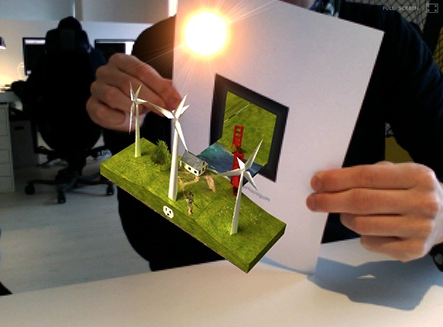
\includegraphics[width=240pt]{chapters/tracking_library_for_the_web/flartoolkit.png}
      \caption{Marker based AR for the web using FLARToolKit.}
      \label{figure:flartoolkit}
    \end{figure}

    \item JSARToolkit: is a JavaScript \cite{International2009} port of FLARToolKit \cite{Yan2011}, operating on canvas images \cite{Canvas2013} and
video element \cite{Hickson2013} contents, provides another marker tracking library. This was the first, open-source, JavaScript \cite{International2009} based, AR solution available for the web. A marker based AR example for the web using JSARToolKit is shown on Figure \ref{figure:jsartoolkit}.

    \begin{figure}[!htb]
      \centering
      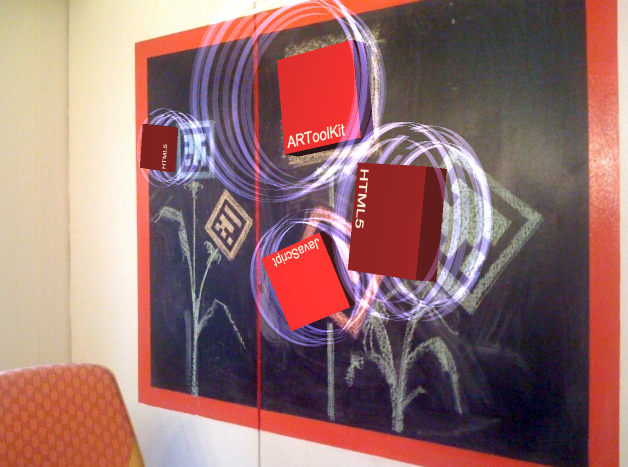
\includegraphics[width=240pt]{chapters/tracking_library_for_the_web/jsartoolkit.png}
      \caption{Marker based AR for the web using JSARToolKit.}
      \label{figure:jsartoolkit}
    \end{figure}

    \item Unifeye Viewer: from Metaio company, offers a robust markerless tracking solution for the web. Unifeye \cite{Metaio2009} also depends on Flash \cite{Flash2013} plugin in order to run on web browsers. A similar example of General Electric's marker based solution, this time markerless based, is shown on Figure \ref{figure:unifeyeviewer}. Note that the 3D image is projected over a magazine cover instead of a fiducial marker \cite{Cho1998}.

    \begin{figure}[!htb]
      \centering
      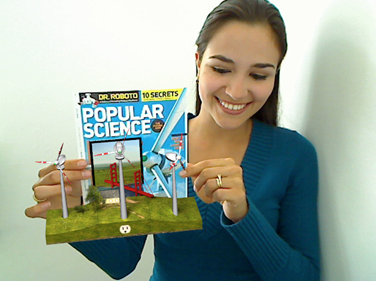
\includegraphics[width=240pt]{chapters/tracking_library_for_the_web/unifeyeviewer.png}
      \caption{Markerless example of image projected over a magazine cover using Unifeye Viewer solution.}
      \label{figure:unifeyeviewer}
    \end{figure}
\end{enumerate}

There is a disadvantage of using marker based AR. Depend on a artificial marker in order to augment the scene with virtual elements is counterintuitive. Commonly, web applications are utilized by novice users that do not have sufficient technical knowledge to perform manual setup, such as print fiducial markers or perform manual initialization for the tracking. FLARToolKit \cite{Yan2011} and JSARToolkit \cite{JSARToolkit2011} are both marker based techniques, using Flash \cite{Flash2013} and JavaScript \cite{International2009}, respectively. FLARToolKit has one more issue which is dependency on Flash \cite{Flash2013} plugin installation. Unifeye Viewer by Metaio, was the only existing solution that provided markerless tracking for the web, although it uses Flash \cite{Flash2013}, excluding it from a potential competitor of \textit{tracking.js}. Markerless tracking techniques do not depend on any artificial marker or advanced user initialization. The space on web targeted AR applications for advertising is gaining more space and the media used in this kind of application needs to be as appealing as possible \cite{Pablo2013}. Making markerless tracking a suitable technique to such applications.

The solution proposed in this thesis, \textit{tracking.js}, provides the first known, open-source, markerless tracking solution for the web that runs entirely in JavaScript \cite{International2009} and HTML5 \cite{Hickson2013}.

% subsection related_work (end)

\subsection{Library Modules} % (fold)
\label{sub:tracking_library_for_the_web:library_modules}

The proposed library is divided in modules in order to allow extension and addition of new features, such as new RA techniques or math utilities. For a better understanding of the library architecture, the current implementation is divided in two packages separating Base from AR classes. Base classes modules are shown in Figure \ref{figure:base_classes} and AR classes in Figure \ref{figure:ar_classes}.

To develop AR applications using only raw JavaScript \cite{International2009} APIs \cite{MDN2013} could be too verbose and complex, \eg\ capturing users' camera and reading its array of pixels. The big amount of steps required for a simple task makes web developers life hard when the goal is to achieve complex implementations. Some level of encapsulation is needed in order to simplify development. The proposed library provides encapsulation for common tasks on the web platform.

The two main available packages splits Base from AR classes. Furthermore, each class of those packages are described. Let's start with the base classes:

\begin{enumerate}
  \item Math: provides common math utilities optimized for the web, such as geometry, linear algebra \cite{Hartley2004} and hamming operations. Typed arrays \cite{TypedArray2013} are used in order to optimize performance, see subsection \ref{sub:basic_concepts:web:javascript_typed_arrays} for more information about typed arrays.
  \item Attribute: allows developers to add attributes to any class through an Attribute interface. The interface adds get and set methods to your class to retrieve and store attribute values, as well as support for change events that can be used to listen for changes in attribute values.
  \item DOMElement: provides a way to create, and manipulate HTML \cite{Hickson2013} DOM nodes \cite{WC2006}. Each DOMElement instance represents an underlying DOM node \cite{WC2006}. In addition to wrapping the basic DOM API \cite{WC2006} and handling cross browser issues, Nodes provide convenient methods for managing styles and subscribing to events.
  \item Canvas: provides an utility class to create, and manipulate HTML5 \cite{Hickson2013} canvas element \cite{Canvas2013}. Each Canvas instance represents an underlying canvas DOM node \cite{Canvas2013}. In addition to wrapping the basic DOM API \cite{WC2006}, also provides methods to extract via \textit{getImageData} method, to loop via \textit{forEach} method, and to set the canvas array of pixels via \textit{setImageData} method.
  \item Video: provides an utility class to create, and manipulate HTML5 \cite{Hickson2013} video element. Each Video instance represents an underlying video DOM node \cite{Canvas2013}. In addition to wrapping the basic DOM API \cite{WC2006}, also provides methods to \textit{play}, \textit{pause} and register tracker algorithms via \textit{track} method. See subsection \ref{sub:basic_concepts:web:audio_and_video} for more information about video element.
  \item VideoCamera: extends all functionalities from Video class with the addition of capturing the user camera via \textit{capture} method. The underlying implementation uses WebRTC \cite{WebRTC2013} and Media Capture and Streams \cite{MediaCapture2013} specifications.
\end{enumerate}

Visual tracking classes includes several computer vision algorithms, such as FAST \cite{RostenFaster2010}, BRIEF \cite{Calonder2010} implementations, homography estimation and others. As the library grows, many other computer vision algorithms are going to be added to the library, such as 3D pose calculation.

\begin{enumerate}
  \item FAST: provides an implementation of Features from Accelerated Segment Test (FAST) \cite{Rosten2010} for features detection via \textit{findCorners(data, threshold)} method, where $data$ is the \textit{ImageData} of the canvas \cite{Canvas2013} frame. It also depends on a $threshold$ argument. The pixel at $p$, see Figure \ref{figure:fast}, is the center of a candidate corner and they are classified if brighter than $p$ by more than the $threshold$.
  \item BRIEF: provides an implementation of Binary Robust Independent Elementary Features (BRIEF) \cite{Calonder2010} for feature extraction via \textit{getDescriptors(data, corners)} method and matching via \textit{match(c1, d1, c2, d2)}, where $data$ is an \textit{ImageData}, and $c1$ and $c2$ are the found corners array return by \textit{FAST.findCorners} method and $d1$ and $d2$ are feature descriptors array return by \textit{BRIEF.getDescriptors} method.
  \item RANSAC: provides an interface used to achieve robust estimation method for homographies and camera pose. There are two available estimation methods implemented that inherits from RANSAC \cite{Hartley2004}, Homography and Pose.
  \item Homography: provides an API to estimate a homography matrix $H$ between images by finding feature correspondences in those images.
  \item Pose: TODO.
  \item ViolaJones: TODO.
  \item Color: TODO.
\end{enumerate}

\begin{figure}[!htb]
    % \tikzumlset{font=\scriptsize}
    \begin{tikzpicture}
        \begin{umlpackage}{Base classes}

            \umlclass[y=-50pt,x=190pt]{Math}{}{
              createIdentityMatrix(size) : Matrix\\
              distance(x1, y1, x2, y2) : Number\\
              getDeterminant(Matrix) : Number\\
              getInverse(Matrix) : Matrix\\
              hammingDistance(n1, n2) : Number\\
              hammingWeight(number) : Number\\
              ...
            }

            \umlclass{Attribute}{}{
              get(name) : Object\\
              set(name, value) : void \\
            }

            \umlclass[y=-100pt]{DOMElement}{
              width : Number\\
              height : Number\\
              visible : boolean\\
            }{
              show() : void\\
              hide() : void \\
            }

            \umlclass[y=-220pt,x=180pt]{Canvas}{
              context : Object
            }{
              forEach(data, callback) : void\\
              getImageData(x, y, width, height) : ImageData \\
              setImageData(data, x, y) : void\\
            }

            \umlclass[y=-335pt]{Video}{}{
              play() : void\\
              pause() : void\\
              track(tracker) : void \\
              getVideoCanvasImageData(x, y, width, height) : ImageData \\
            }

            \umlclass[y=-335pt,x=220pt]{VideoCamera}{}{
              capture() : void \\
            }

        \end{umlpackage}

        \umlinherit[geometry=-|]{DOMElement}{Attribute}
        \umlinherit[geometry=-|]{Canvas}{DOMElement}
        \umlinherit[geometry=-|]{Video}{DOMElement}
        \umlinherit[geometry=|-]{VideoCamera}{Video}
    \end{tikzpicture}
    \caption{Base classes of tracking.js library.}
    \label{figure:base_classes}
\end{figure}

\begin{figure}[!htb]
    % \tikzumlset{font=\scriptsize}
    \begin{tikzpicture}
        \begin{umlpackage}{Visual tracking classes}

            \umlclass{FAST}{}{
              findCorners(data, threshold) : Array\\
            }

            \umlclass[y=-70pt]{BRIEF}{}{
              getDescriptors(data, corners) : Array\\
              match(c1, d1, c2, d2) : Array\\
            }

            \umlclass[y=-150pt]{ViolaJones}{}{
              find() : Array\\
              evalStage() : boolean\\
            }

            \umlclass[y=-225pt]{Color}{}{
              find() : Array\\
            }

            \umlclass[x=200pt]{RANSAC}{}{
              find(matches) : void\\
              score() : Number\\
            }

            \umlclass[y=-90pt,x=200pt]{Homography}{}{
                score(H, matches) : Number\\
            }

            \umlclass[y=-170pt,x=200pt]{Pose}{}{
              find(points2d, points3d) : void\\
            }

        \end{umlpackage}

        \umlinherit[geometry=-|]{Homography}{RANSAC}
        \umlinherit[geometry=-|]{Pose}{RANSAC}
    \end{tikzpicture}
    \caption{Visual tracking classes of tracking.js library.}
    \label{figure:ar_classes}
\end{figure}

\newpage

% subsection library_modules (end)

% section contextualization (end)

\section{Markerless Tracking Algorithm} % (fold)
\label{sec:tracking_library_for_the_web:marker_less_tracking_algorithm}

\subsection{Contextualization} % (fold)
\label{sub:tracking_library_for_the_web:marker_less_tracking_algorithm:contextualization}

Lorem ipsum dolor sit amet, consectetur adipisicing elit.

% subsection contextualization (end)

\subsection{Feature Detector} % (fold)
\label{sub:tracking_library_for_the_web:marker_less_tracking_algorithm:feature_detector}

This technique relies on matching individual features across images and are therefore easy to increase robustness against partial occlusions or matching errors. Illumination invariance is also simple to achieve. Feature points detection is used as the first step of many vision tasks such as tracking, localization, image matching and recognition. In this article we call ``feature'' or ``keypoint'' to refer to a point of interest in two dimensions.

For each frame, the object features are matched by localizing feature templates in search windows around hypothesized locations \cite{Lepetit2005}. The method to extract feature points suggested in Features from Accelerated Segment Test (FAST) \cite{Rosten2010}. FAST \cite{RostenFaster2010} hypothesizes the matches using corner detection. A large number of corner detectors exist in the literature. However, we have a strong interest in real time frame rate applications which computational resources are required requisites. The approach proposed by FAST \cite{RostenFaster2010} allows the detector to produce a suite of high-speed detectors which we currently use for real-time tracking and AR label placement \cite{Calonder2010}. In particular, it is still true that when processing live video streams at full frame rate, existing feature detectors leave little if any time for further processing, even despite the consequences of Moore's Law \cite{Rosten2010}.

To show that speed can been obtained without necessarily sacrificing the quality of the feature detector, in Chapter \ref{cha:evaluation}, we compare our detector, to a variety of well-known detectors. A number of the detectors described below compute a corner response, (1) Edge based corner detectors, corresponds to the boundary between two regions; (2) Gray level derivative based detectors, the assumption that corners exist along edges is an inadequate model for patches of texture and point like features, and is difficult to use at junctions. Therefore a large number of detectors operate directly on gray level images without requiring edge detection; and (3) Direct gray level detectors, Another major class of corner detectors work by examining a small patch of an image to see if it ``looks'' like a corner \cite{Rosten2010}.

The thesis choice was (3) Direct gray level detectors. It works by testing a small patch of an image to see if it could be a corner. The detector is evaluated using a circle surrounding the candidate pixel, the test is based on whether the concentric contiguous arcs around the pixel are significantly different from the central pixel $p$ \cite{Rosten2010}. To classify $p$ as a corner should exists a set of $n$ contiguous pixels in the circle which are all brighter than the intensity of the candidate pixel $I_{p} + t$ (threshold), or all darker than $I_{p} - t$ \cite{Rosten2010}.

The number of contiguous tested pixels could vary accordingly \cite{Rosten2010}, being more common to be FAST-$12$ or FAST-$9$. Empirically, FAST-$9$ showed to have a good repeatability and a better efficiency on the web. The repeatability of found feature points is also important because determines whether the technique is useful in a real-world application.

This detector in itself exhibits high performance, but there are several weaknesses: (1) This high-speed test does not reject as many candidates; (2) The efficiency of the detector will depend on the ordering of the questions and the distribution of corner appearances; and (3) Multiple features are detected adjacent to one another \cite{Rosten2010}.

On Figure \ref{figure:fast}, the highlighted squares are the pixels used in the corner detection. The pixel at $p$ is the central pixel. The arc is indicating that the dashed line passes through FAST-$n$, let $n$ be $9$ or $12$ contiguous pixels which are brighter or darker than $p$ \cite{Rosten2010}.

\begin{figure}[!htb]
  \centering
  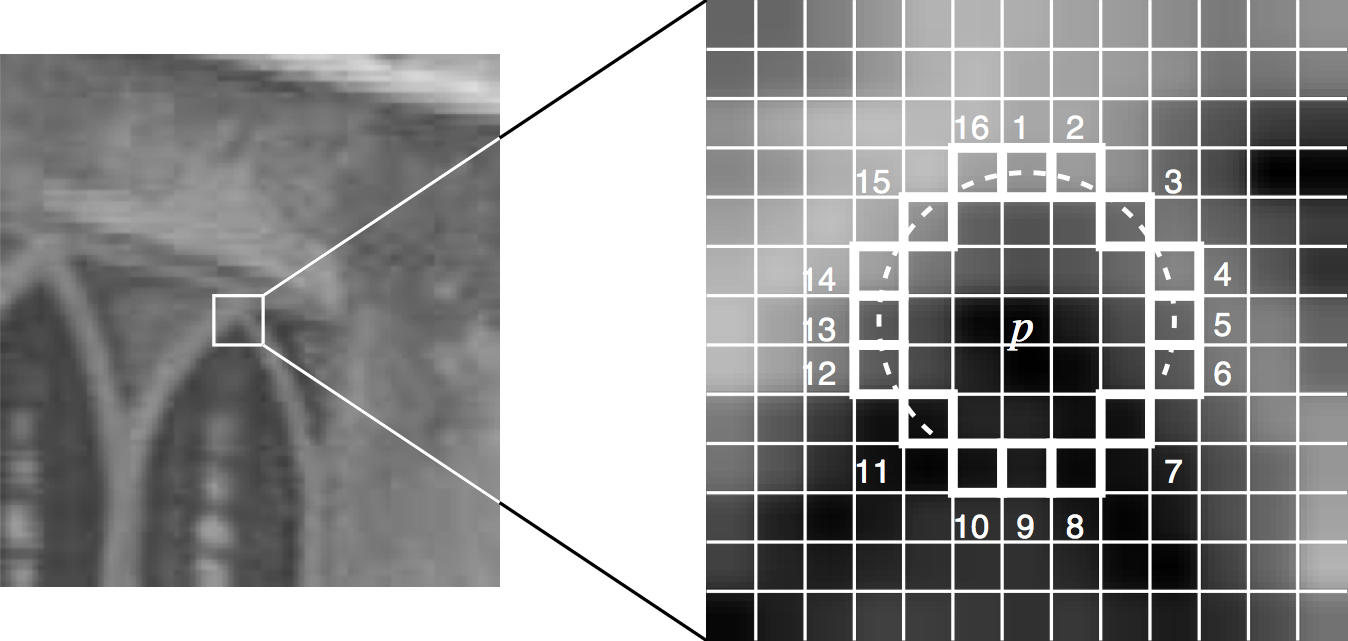
\includegraphics[width=380pt]{chapters/tracking_library_for_the_web/fast.png}
  \caption{Point segment test corner detection in an image patch \cite{Glass2013}.}
  \label{figure:fast}
\end{figure}

% subsection feature_detector (end)

\subsection{Feature Extractors} % (fold)
\label{sub:tracking_library_for_the_web:marker_less_tracking_algorithm:feature_extractors}

To estimate motion, one can then match sets of features \{$m_{i}$\} and \{$m'_{j}$\} extracted from two images taken from similar, and often successive, viewpoints. A classical procedure \cite{Calonder2010} runs as follows. For each point \{$m_{i}$\} in the first image, search in a region of the second image around location \{$m_{i}$\} for point \{$m'_{j}$\}. The search is based on the similarity of the local image windows, also knowns as kernel windows, centered on the points, which strongly characterizes the points when the images are sufficiently close \cite{Lepetit2005}.

\begin{figure}[!htb]
  \centering
  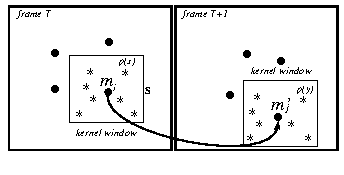
\includegraphics[width=\linewidth]{chapters/tracking_library_for_the_web/BRIEF.pdf}
  \caption{BRIEF \cite{Lepetit2005} feature extractor.}
  \label{figure:BRIEF}
\end{figure}

The feature matching used in the case studies performed in this work search for correspondent points in the current frame. Only points that are highly descriptive invariant features, called keypoints, are tested. Those keypoints were detected using FAST \cite{Rosten2010} in Section \ref{sub:tracking_library_for_the_web:marker_less_tracking_algorithm:feature_detector}. After the keypoints are detected they need to be described and the respective matching point should be found. Since web and handled devices have limited computational power having local descriptors that are fast to compute, to match and being memory efficient are important aspects, for that reason, was used an efficient method called Binary Robust Independent Elementary Features (BRIEF) \cite{Calonder2010}.

To generate the binary string for each key-point found in the smoothed frame, the individual bits are obtained by comparing the intensities of pairs of points, $(\textbf{p}; x, y)$, represented by $\ast$ symbol on Figure \ref{figure:BRIEF}, along the kernel window centered on each key-point without requiring a training phase.
Empirically, this technique shows that $256$ or even $128$ bits \cite{Calonder2010}, often suffice to obtain very good matching results. The best spatial arrangement of the tested (\textbf{x}, \textbf{y})-pairs of points are reach when selected based on an isotropic Gaussian distribution \cite{Calonder2010}. To compute the Gaussian distribution can be time consuming. As an optimization proposed by this article, the Gaussian distribution could be simply replaced by a random function due to its random characteristics.

To generate the binary strings is defined test $\tau$ on patch \textbf{p} of size \textbf{S $\times$ S} as

$$\tau(\textbf{p}; x, y) :=
\begin{cases}
  1 &\mbox{if}\quad \textbf{p(x)} < \textbf{p(y)},\\
  0 &\mbox{otherwise}
\end{cases}$$

where \textbf{p(x)} is the pixel intensity. The set of binary tests is defined by the $n_{d}$ (\textbf{x}, \textbf{y})-location pairs uniquely chosen during the initialization. The $n_{d}$-dimensional bit-string is our BRIEF descriptor for each key-point

$$f_{n_{d}}(\textbf{p}) := \sum_{1 \le i \le n_{d}} 2^{i-1} \tau(\textbf{p}; x, y).$$

In \cite{Calonder2010}, $n_{d}= 128, 256, 512$ were used in the tests and any of those values yield good compromises between speed, storage efficiency, and recognition rate. In this article, $n_{d}= 128$ was used, since it presented good matching results and performance. The number of bytes required to store the descriptor can be calculated by $k = n_{d}/8$, proving that BRIEF is also a memory-efficient method. Detailed results can be found in Chapter \ref{cha:evaluation}.

Once each keypoint is described with its binary string \cite{Calonder2010}, they need to be compared with the closest matching point. Distance metric is critical to the performance of intrusion detection systems. Thus using binary strings reduces the size of the descriptor and provides an interesting data structure that is fast to operate with whose similarity can be measured by the Hamming distance which, on desktop implementations, the computation time could be driven almost to zero using the POPCNT instruction from SSE4.2 \cite{Intel2007}. Only the latest Intel Core i7 CPUs support this instruction.

The Hamming distance is an important step on feature matching, it provides a fast and memory-efficient way to calculate distance between binary strings. Given two image patches $x$ and $y$, denote their binary descriptors as $b(x) \in \{0,1\}^n$ and $b(y) \in \{0,1\}^n$ respectively. Then their Hamming distance is computed by:

$$Ham(x, y)=\sum_{i=1}^{n}b_i(x)\otimes b_i(y)$$

In which $n$ is the dimension of binary descriptor and stands for bitwise XOR operation. According to the definition of Hamming distance, all the elements of a binary descriptor contribute equally to the distance. From the hamming distance, the Hamming weight can be calculated. It is used to find the best feature point match. Here, is generalized the Hamming distance to the weighted Hamming:

$$WHam(x, y)=\sum_{i=1}^{n}w_i(b_i(x)\otimes b_i(y))$$

Where $w_i$ is the weight of the $i$th element. The goal is to learn $w_i,i=1,2\cdots,n$ for the binary descriptor (BRIEF) based on a set of feature points. By assigning different weights to binary codes, what we expect is to obtain a distance space in which the distances of matching patches are less than those of non-matching patches.

% subsection feature_extractors (end)

\subsection{Homography Estimation} % (fold)
\label{sub:tracking_library_for_the_web:marker_less_tracking_algorithm:homography_estimation}

Typically, homographies are estimated between images by finding feature correspondences in those images. A 2D point $(x,y)$ in an image can be represented as a 3D vector $\textbf{x} = (x_1, x_2, x_3)$ where $x = \frac{x_1}{x_3}$ and $y = \frac{x_2}{x_3}$ \cite{Homography2009}. This is called the homogeneous representation of a point and it lies on the projective plane $P^2$. A homography is an invertible mapping of points and lines on the projective plane $P^2$. Hartley and Zisserman \cite{Hartley2004} provide the specific definition that a homography is a mapping from $P^2$ → $P^2$ is a projectivity if and only if there exists a non-singular $3\times3$ matrix $H$ such that for any point in $P^2$ represented by vector $\textbf{x}$ it is true that its mapped point equals $H\textbf{x}$. It should be noted that $H$ can be changed by multiplying by an arbitrary non-zero constant without altering the projective transformation. Thus $H$ is considered a homogeneous matrix and only has $8$ degrees of freedom even though it contains $9$ elements.

The method chosen to solve the homography estimation was the Direct Linear Transformation (DLT) \cite{Impa2009,Hartley2004} algorithm. The DLT algorithm is a simple algorithm used to solve for the homography matrix $H$ given a sufficient set of point correspondences \cite{Homography2009}.

Since we are working in homogeneous coordinates, the relationship between two corresponding points $\textbf{x}$ and $\textbf{x'}$ can be re-written as \cite{Homography2009}:

$$c\begin{pmatrix}u\\ v\\ 1\\\end{pmatrix} = H\begin{pmatrix}x\\ y\\ 1\\\end{pmatrix} \;\; \forall \;\; H=\begin{pmatrix}h1 & h2 & h3\\ h4 & h5 & h6\\ h7 & h8 & h9\\\end{pmatrix},$$

where $c$ is any non-zero constant, $(\; u \; v \; 1 \;)^T$ represents $\textbf{x'}$, $(\; x \; y \; 1 \;)^T$ represents $\textbf{x}$. Dividing the first row of equation (2.1) by the third row and the second row by the third row we get the following two equations \cite{Homography2009}:

\begin{equation}
\label{eq:homography1}
-h1x-h2y-h3 +(h7x+h8y+h9)u=0
\end{equation}
\begin{equation}
\label{eq:homography2}
-h4x-h5y-h6 +(h7x+h8y+h9)u=0
\end{equation}

Equations (\ref{eq:homography1}) and (\ref{eq:homography2}) can be written in matrix form as $A_i\textbf{h}=0$. Where,

$$A_i=\begin{pmatrix}-x & -y & -1 & 0 & 0 & 0 & ux & uy & u\\0 & 0 & 0 & -x & -y & -1 & vx & vy & v\end{pmatrix}$$

and

$$\textbf{h}=\begin{pmatrix}h1 & h2 & h3 & h4 & h5 & h6 & h7 & h8 & h9\end{pmatrix}.$$

Since each point correspondence provides $2$ equations, $4$ correspondences are sufficient to solve for the $8$ degrees of freedom of $H$. JavaScript typed arrays, defined in Section \ref{sub:basic_concepts:web:javascript_typed_arrays}, were used in the homography estimation implementation for better performance results.

% subsection homography_estimation (end)

\subsection{Random Sample Consensus (RANSAC)} % (fold)
\label{sub:tracking_library_for_the_web:marker_less_tracking_algorithm:ransac}

RANSAC (Random Sample Consensus) \cite{Hartley2004} is the most commonly used robust estimation method for homographies according to \cite{Homography2009}. The idea of the algorithm is pretty simple; For a number of iterations, a random sample of $4$ correspondences is selected and a homography $H$ is computed from those four correspondences. Each other correspondence is then classified as an inlier or outlier depending on its concurrence with $H$. After all of the iterations are done, the iteration that contained the largest number of inliers is selected. $H$ can then be recomputed from all of the correspondences that were consider as inliers in that iteration \cite{Homography2009}.

One important step when applying the RANSAC algorithm described above is to decide how to classify correspondences as inliers or outliers. In the implementation for the web only assign the geometric distance \cite{Homography2009} threshold, $t$, between $\textbf{x'}$ and $H\textbf{x}$ was enough. Hartley and Zisserman \cite{Hartley2004} provides more details about RANSAC.

Another issue is to decide how many iterations to run the algorithm, it's not required to try every combination of 4 correspondences. The goal becomes to determine the number of iterations, $N$, that ensures with a probability $p$ that at least one of the random samples will be free from outliers. $N=100$ was used on the web implementation.

% subsection ransac (end)

% section marker_less_tracking_algorithm (end)

\section{Rapid Object Detection (Viola Jones)} % (fold)
\label{sec:tracking_library_for_the_web:rapid_object_detection}

\subsection{Contextualization} % (fold)
\label{sub:tracking_library_for_the_web:rapid_object_detection:contextualization}

Rapid Object Detection \cite{Viola2001} technique, much known as Viola Jones \cite{Viola2001}, brings together new algorithms and insights to construct a library for robust and extremely rapid object detection. What has motivated this technique to be added to \textit{tracking.js} library was the task of face detection. Surprisingly, the algorithm became robust enough to detect any training data \cite{Viola2001}, not only for faces. Currently, \textit{tracking.js} supports, face, eyes, upper body and palm detection.

In order to scan faces, eyes or palm from images, a training phase is required. The training phase generate cascading stages. The cascade are constructed by training classifiers using AdaBoost \cite{Viola2001} and then adjusting the threshold to minimize false negatives. OpenCV library \cite{Bradski2000} has some open-source training data, therefore doubling efforts on training is unnecessary, \ie\ the face training set consisted of 4916 faces, extracted from images downloaded during a random crawl of the world wide web \cite{Viola2001}. Those faces were scaled and aligned to a base resolution of $24$ by $24$ pixels \cite{Viola2001}, see Figure \ref{figure:viola_training}. Training is not the focus of this work, the algorithm to scan the faces is. The training data itself is useless if a Scanning Detector \cite{Viola2001} is not available, the scanning is what makes the rapid object detection.

\begin{figure}[!htb]
  \centering
  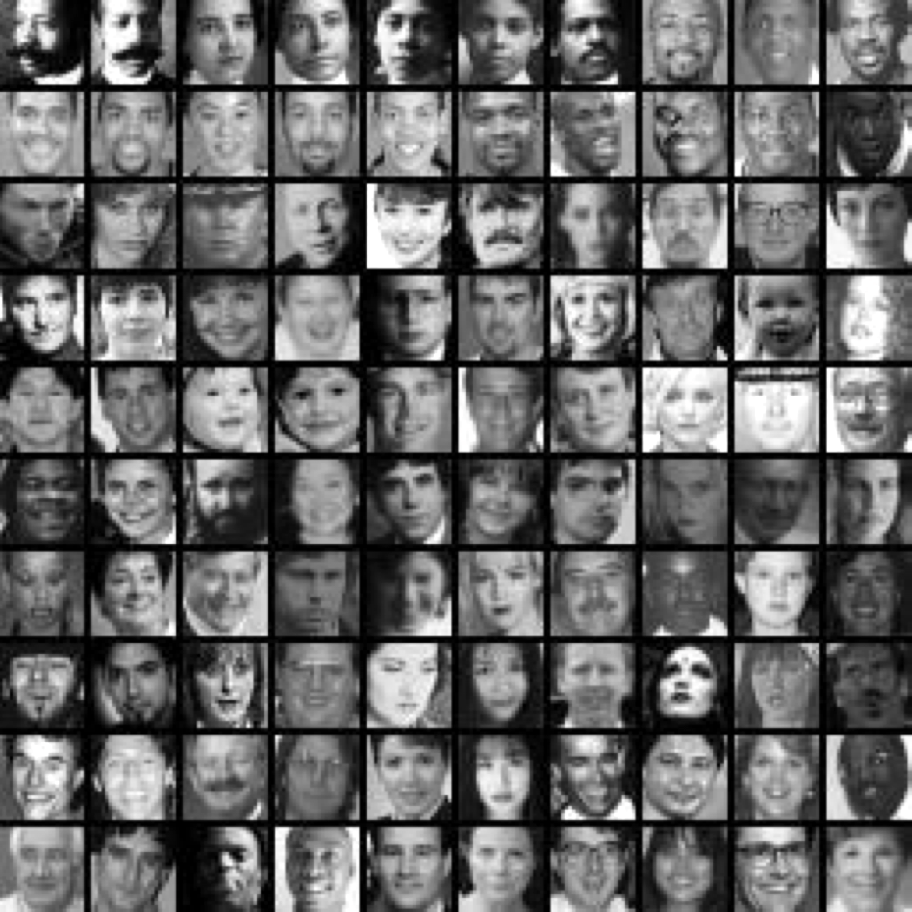
\includegraphics[width=240pt]{chapters/tracking_library_for_the_web/viola_training.png}
  \caption{Example of frontal upright face images used for training \cite{Viola2001}.}
  \label{figure:viola_training}
\end{figure}

A scanning detector was implemented in JavaScript \cite{International2009} and is available on \textit{tracking.js}. The training data used is from OpenCV library \cite{Bradski2000} converted from Extensible Markup Language (XML) \cite{Bray2013} to JavaScript Object Notation (JSON) \cite{Crockford2013}. JSON \cite{Crockford2013} has much superior performance since it's interpreted by JavaScript language \cite{International2009,Crockford2013}. The results of the JavaScript \cite{International2009} implementation can be used in real-time applications, the detector runs at 15 frames per second. For more information about performance see Chapter \ref{cha:evaluation}.

The overall idea of the detection process is that it uses a degenerate decision tree, what Viola and Jones \cite{Viola2001} call ``cascade''. A positive result from the first classifier triggers the evaluation of a second classifier which has also been adjusted to achieve very high detection rates \cite{Viola2001}. A positive result from the second classifier triggers a third classifier, and so on \cite{Viola2001}. The main steps of the scanning algorithm are:

\begin{enumerate}
  \item Create or scale a squared block, initially set to $20\times20$ pixels, by $1.25$ per iteration;
  \item Loop the squared block by $\Delta$ pixels over the image;
  \item For each squared block location, loop the decision tree and evaluate each stage;
  \item A positive result of the stage \cite{Viola2001} triggers the next stage, otherwise stops the stages loop;
  \item If all stages were positively evaluated store that rectangle as a possible face;
  \item Once the decision tree is done, group the overlapping rectangles;
  \item Find the best rectangle of each the group to represent the face. This phase is also known as ``merging phase''.
\end{enumerate}

The final detector is scanned across the image at multiple scales and locations of the image. This process makes sense because the features can be evaluated at any scale with the same cost \cite{Viola2001}. Good results were obtained using a set of scales a factor of $1.25$. Subsequent locations are obtained by shifting the window some number of pixels $\Delta$, for a better accuracy $\Delta=1$ is recommended. We can achieve a significant speedup by setting $\Delta=2$ with only a slight decrease in accuracy, thus this value was set as default value of the JavaScript \cite{International2009} implementation.

Viola and Jones \cite{Viola2001} proposed that for each found possible rectangle representing the face to be partitioned into disjoint subsets data structures. Two detections are in the same subset if their bounding regions overlap \cite{Viola2001}. The corners of the final bounding region are the average of the corners of all detections in the set. In order to perform well on the web, some optimizations were made in the implementation level of the scanning detector. The disjoint set was replaced by an alternative logic that is called ``Minimum Neighbor Area Grouping'' by this thesis. Minimum Neighbor Area Grouping has $O(N^2)$ performance \cite{black2007big} and consists in a loop trough the possible rectangle faces returned by the scanning detector. For each step of the loop compare the current rectangle with all other not yet compared rectangles. If the rectangle area overlaps more than $\eta$ with the compared, by default $\eta=0.5$ (or $50\%$), select the smallest rectangle in area of the comparison. Using the smallest rectangle, guarantees that the best match is much centralized in the face.

For more information about the JavaScript \cite{International2009} implementation, such as evaluation and results, see Chapter \ref{cha:evaluation}.

% subsection contextualization (end)

% section rapid_object_detection (end)

\section{Color Tracking Algorithm} % (fold)
\label{sec:tracking_library_for_the_web:color_tracking_algorithm}

\subsection{Contextualization} % (fold)
\label{sub:tracking_library_for_the_web:color_tracking_algorithm:contextualization}

Colors are part of our lives, they are everywhere in every single object. Being able to use colored objects to control your browser using the user camera is very appealing. For that reason, \textit{training.js} implemented a basic color tracking algorithm that resulted in an real-time frame rate trough a simple and intuitive API.

% subsection contextualization (end)

% section color_tracking_algorithm (end)

% chapter tracking_library_for_the_web (end)
\chapter{Tracking Library for the Web (tracking.js)} % (fold)
\label{cha:tracking_library_for_the_web}

\section{Contextualization} % (fold)
\label{sec:tracking_library_for_the_web:Contextualization}

The desktop platform is the target environment most commonly addressed when developing AR systems. However, depending on the requirements of an AR application, the use of different execution platforms may be necessary. If the system has to be published to several users, the web platform shows to be more adequate, where the application is executed through the Internet in a web browser \cite{Pablo2013}.
The use of markerless tracking, which is based on natural features of the scene, has also been gaining more space on web targeted AR applications for advertising. The media used in this kind of application needs to be as appealing as possible in order to catch consumers' attention. Markerless tracking satisfies this requirement, since the idea of having a real scene augmented with virtual objects without any artificial elements such as markers added to the environment is very attractive \cite{Pablo2013}. In addition, the product being advertised can be tracked and augmented with virtual elements \cite{Pablo2013}.
Browsers are evolving very fast when compared to the the previous decade \cite{Hickson2013}. JavaScript language \cite{International2009,MDN2013} wasn't prepared to handle typed data structures \cite{TypedArray2013} able to manipulate raw binary data safely \cite{Canvas2013}, all the computational complexity required by AR algorithms was too much for that growing environment. Browsers weren't able to capture audio and video \cite{MediaCapture2013,WebRTC2013} natively, without plugin installation \cite{Flash2013}, an essential feature for AR applications. This reality has changed, this involves the use of several modern browser specifications \cite{Hickson2013,WC2006} as well as implementation of different computer vision algorithms and techniques into the browser environment taking advantage of all those modern APIs \cite{Hickson2013,WC2006}.

In this context, this thesis aims to present the implementation and evaluation of a solution regarding tracking techniques for web targeted AR. The available algorithms and techniques can be used for different applications, such as, detect faces, identify objects and colors and track moving objects. The solution is called \textit{tracking.js}. Some optimizations are discussed and implemented on this work in order to achieve good results when compared with similar implementations in compiled languages.

\subsection{Related Work} % (fold)
\label{sub:tracking_library_for_the_web:related_work}

There are not many web based RA solutions available and registered in the literature. The ones available are mainly focused on fiducial markers \cite{Cho1998}, such as FLARToolKit \cite{Yan2011} and JSARToolkit \cite{JSARToolkit2011}, they both are ports of ARToolKit \cite{Hirokazu2002}. ARToolKit is a desktop library which is useful to make vision-based AR applications \cite{Hirokazu2002}. The Metaio company developed Unifeye Viewer \cite{Metaio2009}, a proprietary plug-in for Flash \cite{Flash2013} that allows the utilization of markerless AR applications on the web. In order to run Flash \cite{Flash2013} based applications, the installation of its plugin is required. Third-party plugins, such as Flash \cite{Flash2013}, are in decadency on modern and mobile web browsers, instead JavaScript \cite{International2009} based solutions are preferred, since they can run in any modern browser without requiring any user effort of installing external software. Some smart-phones don't even support Flash \cite{Flash2013} plugin into their browsers, \eg\ Safari for mobile \cite{Safari2013} is one example of a mobile browser that has banned Flash \cite{Flash2013}.

\begin{enumerate}
    \item FLARToolKit: is a port of the well-known ARToolKit \cite{Hirokazu2002} marker tracking library to ActionScript \cite{Flash2013}, which is the language utilized in the development of Flash \cite{Flash2013} applications for the web. This was the first initiative towards AR solutions for the web \cite{Pablo2013}. Using FLARToolKit \cite{Yan2011}, is possible to develop AR applications that runs on client's browser. A marker based AR example for the web, developed for a marketing campaign of General Electric's company using FLARToolKit, is shown on Figure \ref{figure:flartoolkit}.

    \begin{figure}[!htb]
      \centering
      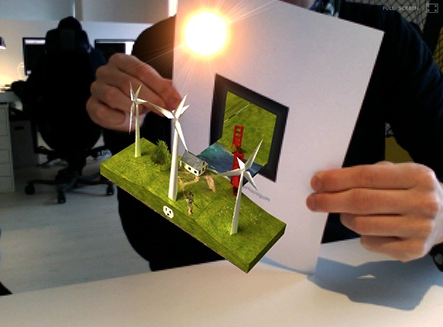
\includegraphics[width=240pt]{chapters/tracking_library_for_the_web/flartoolkit.png}
      \caption{Marker based AR for the web using FLARToolKit.}
      \label{figure:flartoolkit}
    \end{figure}

    \item JSARToolkit: is a JavaScript \cite{International2009} port of FLARToolKit \cite{Yan2011}, operating on canvas images \cite{Canvas2013} and
video element \cite{Hickson2013} contents, provides another marker tracking library. This was the first, open-source, JavaScript \cite{International2009} based, AR solution available for the web. A marker based AR example for the web using JSARToolKit is shown on Figure \ref{figure:jsartoolkit}.

    \begin{figure}[!htb]
      \centering
      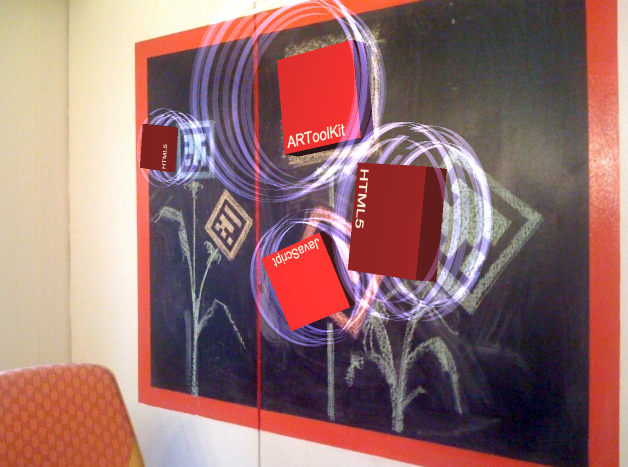
\includegraphics[width=240pt]{chapters/tracking_library_for_the_web/jsartoolkit.png}
      \caption{Marker based AR for the web using JSARToolKit.}
      \label{figure:jsartoolkit}
    \end{figure}

    \item Unifeye Viewer: from Metaio company, offers a robust markerless tracking solution for the web. Unifeye \cite{Metaio2009} also depends on Flash \cite{Flash2013} plugin in order to run on web browsers. A similar example of General Electric's marker based solution, this time markerless based, is shown on Figure \ref{figure:unifeyeviewer}. Note that the 3D image is projected over a magazine cover instead of a fiducial marker \cite{Cho1998}.

    \begin{figure}[!htb]
      \centering
      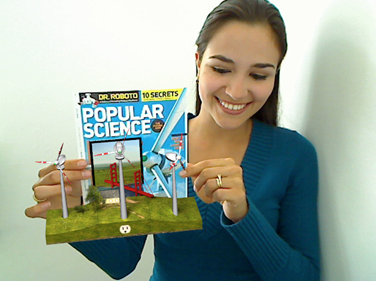
\includegraphics[width=240pt]{chapters/tracking_library_for_the_web/unifeyeviewer.png}
      \caption{Markerless example of image projected over a magazine cover using Unifeye Viewer solution.}
      \label{figure:unifeyeviewer}
    \end{figure}
\end{enumerate}

There is a disadvantage of using marker based AR. Depend on a artificial marker in order to augment the scene with virtual elements is counterintuitive. Commonly, web applications are utilized by novice users that do not have sufficient technical knowledge to perform manual setup, such as print fiducial markers or perform manual initialization for the tracking. FLARToolKit \cite{Yan2011} and JSARToolkit \cite{JSARToolkit2011} are both marker based techniques, using Flash \cite{Flash2013} and JavaScript \cite{International2009}, respectively. FLARToolKit has one more issue which is dependency on Flash \cite{Flash2013} plugin installation. Unifeye Viewer by Metaio, was the only existing solution that provided markerless tracking for the web, although it uses Flash \cite{Flash2013}, excluding it from a potential competitor of \textit{tracking.js}. Markerless tracking techniques do not depend on any artificial marker or advanced user initialization. The space on web targeted AR applications for advertising is gaining more space and the media used in this kind of application needs to be as appealing as possible \cite{Pablo2013}. Making markerless tracking a suitable technique to such applications.

The solution proposed in this thesis, \textit{tracking.js}, provides the first known, open-source, markerless tracking solution for the web that runs entirely in JavaScript \cite{International2009} and HTML5 \cite{Hickson2013}.

% subsection related_work (end)

\subsection{Library Modules} % (fold)
\label{sub:tracking_library_for_the_web:library_modules}

The proposed library is divided in modules in order to allow extension and addition of new features, such as new RA techniques or math utilities. For a better understanding of the library architecture, the current implementation is divided in two packages separating Base from AR classes. Base classes modules are shown in Figure \ref{figure:base_classes} and AR classes in Figure \ref{figure:ar_classes}.

To develop AR applications using only raw JavaScript \cite{International2009} APIs \cite{MDN2013} could be too verbose and complex, \eg\ capturing users' camera and reading its array of pixels. The big amount of steps required for a simple task makes web developers life hard when the goal is to achieve complex implementations. Some level of encapsulation is needed in order to simplify development. The proposed library provides encapsulation for common tasks on the web platform.

The two main available packages splits Base from AR classes. Furthermore, each class of those packages are described. Let's start with the base classes:

\begin{enumerate}
  \item Math: provides common math utilities optimized for the web, such as geometry, linear algebra \cite{Hartley2004} and hamming operations. Typed arrays \cite{TypedArray2013} are used in order to optimize performance, see subsection \ref{sub:basic_concepts:web:javascript_typed_arrays} for more information about typed arrays.
  \item Attribute: allows developers to add attributes to any class through an Attribute interface. The interface adds get and set methods to your class to retrieve and store attribute values, as well as support for change events that can be used to listen for changes in attribute values.
  \item DOMElement: provides a way to create, and manipulate HTML \cite{Hickson2013} DOM nodes \cite{WC2006}. Each DOMElement instance represents an underlying DOM node \cite{WC2006}. In addition to wrapping the basic DOM API \cite{WC2006} and handling cross browser issues, Nodes provide convenient methods for managing styles and subscribing to events.
  \item Canvas: provides an utility class to create, and manipulate HTML5 \cite{Hickson2013} canvas element \cite{Canvas2013}. Each Canvas instance represents an underlying canvas DOM node \cite{Canvas2013}. In addition to wrapping the basic DOM API \cite{WC2006}, also provides methods to extract via \textit{getImageData} method, to loop via \textit{forEach} method, and to set the canvas array of pixels via \textit{setImageData} method.
  \item Video: provides an utility class to create, and manipulate HTML5 \cite{Hickson2013} video element. Each Video instance represents an underlying video DOM node \cite{Canvas2013}. In addition to wrapping the basic DOM API \cite{WC2006}, also provides methods to \textit{play}, \textit{pause} and register tracker algorithms via \textit{track} method. See subsection \ref{sub:basic_concepts:web:audio_and_video} for more information about video element.
  \item VideoCamera: extends all functionalities from Video class with the addition of capturing the user camera via \textit{capture} method. The underlying implementation uses WebRTC \cite{WebRTC2013} and Media Capture and Streams \cite{MediaCapture2013} specifications.
\end{enumerate}

Visual tracking classes includes several computer vision algorithms, such as FAST \cite{RostenFaster2010}, BRIEF \cite{Calonder2010} implementations, homography estimation and others. As the library grows, many other computer vision algorithms are going to be added to the library, such as 3D pose calculation.

\begin{enumerate}
  \item FAST: provides an implementation of Features from Accelerated Segment Test (FAST) \cite{Rosten2010} for features detection via \textit{findCorners(data, threshold)} method, where $data$ is the \textit{ImageData} of the canvas \cite{Canvas2013} frame. It also depends on a $threshold$ argument. The pixel at $p$, see Figure \ref{figure:fast}, is the center of a candidate corner and they are classified if brighter than $p$ by more than the $threshold$.
  \item BRIEF: provides an implementation of Binary Robust Independent Elementary Features (BRIEF) \cite{Calonder2010} for feature extraction via \textit{getDescriptors(data, corners)} method and matching via \textit{match(c1, d1, c2, d2)}, where $data$ is an \textit{ImageData}, and $c1$ and $c2$ are the found corners array return by \textit{FAST.findCorners} method and $d1$ and $d2$ are feature descriptors array return by \textit{BRIEF.getDescriptors} method.
  \item RANSAC: provides an interface used to achieve robust estimation method for homographies and camera pose. There are two available estimation methods implemented that inherits from RANSAC \cite{Hartley2004}, Homography and Pose.
  \item Homography: provides an API to estimate a homography matrix $H$ between images by finding feature correspondences in those images.
  \item Pose: TODO.
  \item ViolaJones: TODO.
  \item Color: TODO.
\end{enumerate}

\begin{figure}[!htb]
    % \tikzumlset{font=\scriptsize}
    \begin{tikzpicture}
        \begin{umlpackage}{Base classes}

            \umlclass[y=-50pt,x=190pt]{Math}{}{
              createIdentityMatrix(size) : Matrix\\
              distance(x1, y1, x2, y2) : Number\\
              getDeterminant(Matrix) : Number\\
              getInverse(Matrix) : Matrix\\
              hammingDistance(n1, n2) : Number\\
              hammingWeight(number) : Number\\
              ...
            }

            \umlclass{Attribute}{}{
              get(name) : Object\\
              set(name, value) : void \\
            }

            \umlclass[y=-100pt]{DOMElement}{
              width : Number\\
              height : Number\\
              visible : boolean\\
            }{
              show() : void\\
              hide() : void \\
            }

            \umlclass[y=-220pt,x=180pt]{Canvas}{
              context : Object
            }{
              forEach(data, callback) : void\\
              getImageData(x, y, width, height) : ImageData \\
              setImageData(data, x, y) : void\\
            }

            \umlclass[y=-335pt]{Video}{}{
              play() : void\\
              pause() : void\\
              track(tracker) : void \\
              getVideoCanvasImageData(x, y, width, height) : ImageData \\
            }

            \umlclass[y=-335pt,x=220pt]{VideoCamera}{}{
              capture() : void \\
            }

        \end{umlpackage}

        \umlinherit[geometry=-|]{DOMElement}{Attribute}
        \umlinherit[geometry=-|]{Canvas}{DOMElement}
        \umlinherit[geometry=-|]{Video}{DOMElement}
        \umlinherit[geometry=|-]{VideoCamera}{Video}
    \end{tikzpicture}
    \caption{Base classes of tracking.js library.}
    \label{figure:base_classes}
\end{figure}

\begin{figure}[!htb]
    % \tikzumlset{font=\scriptsize}
    \begin{tikzpicture}
        \begin{umlpackage}{Visual tracking classes}

            \umlclass{FAST}{}{
              findCorners(data, threshold) : Array\\
            }

            \umlclass[y=-70pt]{BRIEF}{}{
              getDescriptors(data, corners) : Array\\
              match(c1, d1, c2, d2) : Array\\
            }

            \umlclass[y=-150pt]{ViolaJones}{}{
              find() : Array\\
              evalStage() : boolean\\
            }

            \umlclass[y=-225pt]{Color}{}{
              find() : Array\\
            }

            \umlclass[x=200pt]{RANSAC}{}{
              find(matches) : void\\
              score() : Number\\
            }

            \umlclass[y=-90pt,x=200pt]{Homography}{}{
                score(H, matches) : Number\\
            }

            \umlclass[y=-170pt,x=200pt]{Pose}{}{
              find(points2d, points3d) : void\\
            }

        \end{umlpackage}

        \umlinherit[geometry=-|]{Homography}{RANSAC}
        \umlinherit[geometry=-|]{Pose}{RANSAC}
    \end{tikzpicture}
    \caption{Visual tracking classes of tracking.js library.}
    \label{figure:ar_classes}
\end{figure}

\newpage

% subsection library_modules (end)

% section contextualization (end)

\section{Markerless Tracking Algorithm} % (fold)
\label{sec:tracking_library_for_the_web:marker_less_tracking_algorithm}

\subsection{Contextualization} % (fold)
\label{sub:tracking_library_for_the_web:marker_less_tracking_algorithm:contextualization}

Lorem ipsum dolor sit amet, consectetur adipisicing elit.

% subsection contextualization (end)

\subsection{Feature Detector} % (fold)
\label{sub:tracking_library_for_the_web:marker_less_tracking_algorithm:feature_detector}

This technique relies on matching individual features across images and are therefore easy to increase robustness against partial occlusions or matching errors. Illumination invariance is also simple to achieve. Feature points detection is used as the first step of many vision tasks such as tracking, localization, image matching and recognition. In this article we call ``feature'' or ``keypoint'' to refer to a point of interest in two dimensions.

For each frame, the object features are matched by localizing feature templates in search windows around hypothesized locations \cite{Lepetit2005}. The method to extract feature points suggested in Features from Accelerated Segment Test (FAST) \cite{Rosten2010}. FAST \cite{RostenFaster2010} hypothesizes the matches using corner detection. A large number of corner detectors exist in the literature. However, we have a strong interest in real time frame rate applications which computational resources are required requisites. The approach proposed by FAST \cite{RostenFaster2010} allows the detector to produce a suite of high-speed detectors which we currently use for real-time tracking and AR label placement \cite{Calonder2010}. In particular, it is still true that when processing live video streams at full frame rate, existing feature detectors leave little if any time for further processing, even despite the consequences of Moore's Law \cite{Rosten2010}.

To show that speed can been obtained without necessarily sacrificing the quality of the feature detector, in Chapter \ref{cha:evaluation}, we compare our detector, to a variety of well-known detectors. A number of the detectors described below compute a corner response, (1) Edge based corner detectors, corresponds to the boundary between two regions; (2) Gray level derivative based detectors, the assumption that corners exist along edges is an inadequate model for patches of texture and point like features, and is difficult to use at junctions. Therefore a large number of detectors operate directly on gray level images without requiring edge detection; and (3) Direct gray level detectors, Another major class of corner detectors work by examining a small patch of an image to see if it ``looks'' like a corner \cite{Rosten2010}.

The thesis choice was (3) Direct gray level detectors. It works by testing a small patch of an image to see if it could be a corner. The detector is evaluated using a circle surrounding the candidate pixel, the test is based on whether the concentric contiguous arcs around the pixel are significantly different from the central pixel $p$ \cite{Rosten2010}. To classify $p$ as a corner should exists a set of $n$ contiguous pixels in the circle which are all brighter than the intensity of the candidate pixel $I_{p} + t$ (threshold), or all darker than $I_{p} - t$ \cite{Rosten2010}.

The number of contiguous tested pixels could vary accordingly \cite{Rosten2010}, being more common to be FAST-$12$ or FAST-$9$. Empirically, FAST-$9$ showed to have a good repeatability and a better efficiency on the web. The repeatability of found feature points is also important because determines whether the technique is useful in a real-world application.

This detector in itself exhibits high performance, but there are several weaknesses: (1) This high-speed test does not reject as many candidates; (2) The efficiency of the detector will depend on the ordering of the questions and the distribution of corner appearances; and (3) Multiple features are detected adjacent to one another \cite{Rosten2010}.

On Figure \ref{figure:fast}, the highlighted squares are the pixels used in the corner detection. The pixel at $p$ is the central pixel. The arc is indicating that the dashed line passes through FAST-$n$, let $n$ be $9$ or $12$ contiguous pixels which are brighter or darker than $p$ \cite{Rosten2010}.

\begin{figure}[!htb]
  \centering
  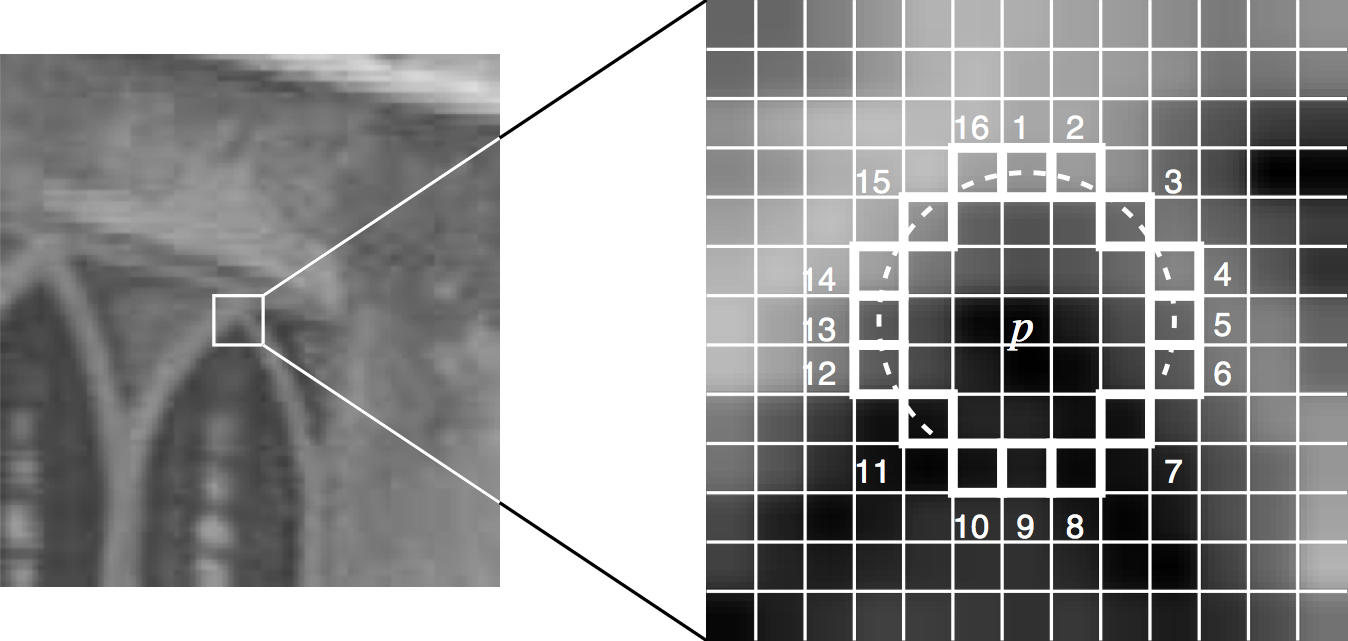
\includegraphics[width=380pt]{chapters/tracking_library_for_the_web/fast.png}
  \caption{Point segment test corner detection in an image patch \cite{Glass2013}.}
  \label{figure:fast}
\end{figure}

% subsection feature_detector (end)

\subsection{Feature Extractors} % (fold)
\label{sub:tracking_library_for_the_web:marker_less_tracking_algorithm:feature_extractors}

To estimate motion, one can then match sets of features \{$m_{i}$\} and \{$m'_{j}$\} extracted from two images taken from similar, and often successive, viewpoints. A classical procedure \cite{Calonder2010} runs as follows. For each point \{$m_{i}$\} in the first image, search in a region of the second image around location \{$m_{i}$\} for point \{$m'_{j}$\}. The search is based on the similarity of the local image windows, also knowns as kernel windows, centered on the points, which strongly characterizes the points when the images are sufficiently close \cite{Lepetit2005}.

\begin{figure}[!htb]
  \centering
  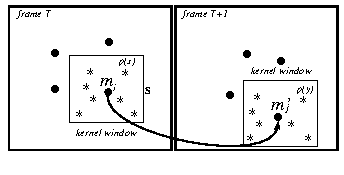
\includegraphics[width=\linewidth]{chapters/tracking_library_for_the_web/BRIEF.pdf}
  \caption{BRIEF \cite{Lepetit2005} feature extractor.}
  \label{figure:BRIEF}
\end{figure}

The feature matching used in the case studies performed in this work search for correspondent points in the current frame. Only points that are highly descriptive invariant features, called keypoints, are tested. Those keypoints were detected using FAST \cite{Rosten2010} in Section \ref{sub:tracking_library_for_the_web:marker_less_tracking_algorithm:feature_detector}. After the keypoints are detected they need to be described and the respective matching point should be found. Since web and handled devices have limited computational power having local descriptors that are fast to compute, to match and being memory efficient are important aspects, for that reason, was used an efficient method called Binary Robust Independent Elementary Features (BRIEF) \cite{Calonder2010}.

To generate the binary string for each key-point found in the smoothed frame, the individual bits are obtained by comparing the intensities of pairs of points, $(\textbf{p}; x, y)$, represented by $\ast$ symbol on Figure \ref{figure:BRIEF}, along the kernel window centered on each key-point without requiring a training phase.
Empirically, this technique shows that $256$ or even $128$ bits \cite{Calonder2010}, often suffice to obtain very good matching results. The best spatial arrangement of the tested (\textbf{x}, \textbf{y})-pairs of points are reach when selected based on an isotropic Gaussian distribution \cite{Calonder2010}. To compute the Gaussian distribution can be time consuming. As an optimization proposed by this article, the Gaussian distribution could be simply replaced by a random function due to its random characteristics.

To generate the binary strings is defined test $\tau$ on patch \textbf{p} of size \textbf{S $\times$ S} as

$$\tau(\textbf{p}; x, y) :=
\begin{cases}
  1 &\mbox{if}\quad \textbf{p(x)} < \textbf{p(y)},\\
  0 &\mbox{otherwise}
\end{cases}$$

where \textbf{p(x)} is the pixel intensity. The set of binary tests is defined by the $n_{d}$ (\textbf{x}, \textbf{y})-location pairs uniquely chosen during the initialization. The $n_{d}$-dimensional bit-string is our BRIEF descriptor for each key-point

$$f_{n_{d}}(\textbf{p}) := \sum_{1 \le i \le n_{d}} 2^{i-1} \tau(\textbf{p}; x, y).$$

In \cite{Calonder2010}, $n_{d}= 128, 256, 512$ were used in the tests and any of those values yield good compromises between speed, storage efficiency, and recognition rate. In this article, $n_{d}= 128$ was used, since it presented good matching results and performance. The number of bytes required to store the descriptor can be calculated by $k = n_{d}/8$, proving that BRIEF is also a memory-efficient method. Detailed results can be found in Chapter \ref{cha:evaluation}.

Once each keypoint is described with its binary string \cite{Calonder2010}, they need to be compared with the closest matching point. Distance metric is critical to the performance of intrusion detection systems. Thus using binary strings reduces the size of the descriptor and provides an interesting data structure that is fast to operate with whose similarity can be measured by the Hamming distance which, on desktop implementations, the computation time could be driven almost to zero using the POPCNT instruction from SSE4.2 \cite{Intel2007}. Only the latest Intel Core i7 CPUs support this instruction.

The Hamming distance is an important step on feature matching, it provides a fast and memory-efficient way to calculate distance between binary strings. Given two image patches $x$ and $y$, denote their binary descriptors as $b(x) \in \{0,1\}^n$ and $b(y) \in \{0,1\}^n$ respectively. Then their Hamming distance is computed by:

$$Ham(x, y)=\sum_{i=1}^{n}b_i(x)\otimes b_i(y)$$

In which $n$ is the dimension of binary descriptor and stands for bitwise XOR operation. According to the definition of Hamming distance, all the elements of a binary descriptor contribute equally to the distance. From the hamming distance, the Hamming weight can be calculated. It is used to find the best feature point match. Here, is generalized the Hamming distance to the weighted Hamming:

$$WHam(x, y)=\sum_{i=1}^{n}w_i(b_i(x)\otimes b_i(y))$$

Where $w_i$ is the weight of the $i$th element. The goal is to learn $w_i,i=1,2\cdots,n$ for the binary descriptor (BRIEF) based on a set of feature points. By assigning different weights to binary codes, what we expect is to obtain a distance space in which the distances of matching patches are less than those of non-matching patches.

% subsection feature_extractors (end)

\subsection{Homography Estimation} % (fold)
\label{sub:tracking_library_for_the_web:marker_less_tracking_algorithm:homography_estimation}

Typically, homographies are estimated between images by finding feature correspondences in those images. A 2D point $(x,y)$ in an image can be represented as a 3D vector $\textbf{x} = (x_1, x_2, x_3)$ where $x = \frac{x_1}{x_3}$ and $y = \frac{x_2}{x_3}$ \cite{Homography2009}. This is called the homogeneous representation of a point and it lies on the projective plane $P^2$. A homography is an invertible mapping of points and lines on the projective plane $P^2$. Hartley and Zisserman \cite{Hartley2004} provide the specific definition that a homography is a mapping from $P^2$ → $P^2$ is a projectivity if and only if there exists a non-singular $3\times3$ matrix $H$ such that for any point in $P^2$ represented by vector $\textbf{x}$ it is true that its mapped point equals $H\textbf{x}$. It should be noted that $H$ can be changed by multiplying by an arbitrary non-zero constant without altering the projective transformation. Thus $H$ is considered a homogeneous matrix and only has $8$ degrees of freedom even though it contains $9$ elements.

The method chosen to solve the homography estimation was the Direct Linear Transformation (DLT) \cite{Impa2009,Hartley2004} algorithm. The DLT algorithm is a simple algorithm used to solve for the homography matrix $H$ given a sufficient set of point correspondences \cite{Homography2009}.

Since we are working in homogeneous coordinates, the relationship between two corresponding points $\textbf{x}$ and $\textbf{x'}$ can be re-written as \cite{Homography2009}:

$$c\begin{pmatrix}u\\ v\\ 1\\\end{pmatrix} = H\begin{pmatrix}x\\ y\\ 1\\\end{pmatrix} \;\; \forall \;\; H=\begin{pmatrix}h1 & h2 & h3\\ h4 & h5 & h6\\ h7 & h8 & h9\\\end{pmatrix},$$

where $c$ is any non-zero constant, $(\; u \; v \; 1 \;)^T$ represents $\textbf{x'}$, $(\; x \; y \; 1 \;)^T$ represents $\textbf{x}$. Dividing the first row of equation (2.1) by the third row and the second row by the third row we get the following two equations \cite{Homography2009}:

\begin{equation}
\label{eq:homography1}
-h1x-h2y-h3 +(h7x+h8y+h9)u=0
\end{equation}
\begin{equation}
\label{eq:homography2}
-h4x-h5y-h6 +(h7x+h8y+h9)u=0
\end{equation}

Equations (\ref{eq:homography1}) and (\ref{eq:homography2}) can be written in matrix form as $A_i\textbf{h}=0$. Where,

$$A_i=\begin{pmatrix}-x & -y & -1 & 0 & 0 & 0 & ux & uy & u\\0 & 0 & 0 & -x & -y & -1 & vx & vy & v\end{pmatrix}$$

and

$$\textbf{h}=\begin{pmatrix}h1 & h2 & h3 & h4 & h5 & h6 & h7 & h8 & h9\end{pmatrix}.$$

Since each point correspondence provides $2$ equations, $4$ correspondences are sufficient to solve for the $8$ degrees of freedom of $H$. JavaScript typed arrays, defined in Section \ref{sub:basic_concepts:web:javascript_typed_arrays}, were used in the homography estimation implementation for better performance results.

% subsection homography_estimation (end)

\subsection{Random Sample Consensus (RANSAC)} % (fold)
\label{sub:tracking_library_for_the_web:marker_less_tracking_algorithm:ransac}

RANSAC (Random Sample Consensus) \cite{Hartley2004} is the most commonly used robust estimation method for homographies according to \cite{Homography2009}. The idea of the algorithm is pretty simple; For a number of iterations, a random sample of $4$ correspondences is selected and a homography $H$ is computed from those four correspondences. Each other correspondence is then classified as an inlier or outlier depending on its concurrence with $H$. After all of the iterations are done, the iteration that contained the largest number of inliers is selected. $H$ can then be recomputed from all of the correspondences that were consider as inliers in that iteration \cite{Homography2009}.

One important step when applying the RANSAC algorithm described above is to decide how to classify correspondences as inliers or outliers. In the implementation for the web only assign the geometric distance \cite{Homography2009} threshold, $t$, between $\textbf{x'}$ and $H\textbf{x}$ was enough. Hartley and Zisserman \cite{Hartley2004} provides more details about RANSAC.

Another issue is to decide how many iterations to run the algorithm, it's not required to try every combination of 4 correspondences. The goal becomes to determine the number of iterations, $N$, that ensures with a probability $p$ that at least one of the random samples will be free from outliers. $N=100$ was used on the web implementation.

% subsection ransac (end)

% section marker_less_tracking_algorithm (end)

\section{Rapid Object Detection (Viola Jones)} % (fold)
\label{sec:tracking_library_for_the_web:rapid_object_detection}

\subsection{Contextualization} % (fold)
\label{sub:tracking_library_for_the_web:rapid_object_detection:contextualization}

Rapid Object Detection \cite{Viola2001} technique, much known as Viola Jones \cite{Viola2001}, brings together new algorithms and insights to construct a library for robust and extremely rapid object detection. What has motivated this technique to be added to \textit{tracking.js} library was the task of face detection. Surprisingly, the algorithm became robust enough to detect any training data \cite{Viola2001}, not only for faces. Currently, \textit{tracking.js} supports, face, eyes, upper body and palm detection.

In order to scan faces, eyes or palm from images, a training phase is required. The training phase generate cascading stages. The cascade are constructed by training classifiers using AdaBoost \cite{Viola2001} and then adjusting the threshold to minimize false negatives. OpenCV library \cite{Bradski2000} has some open-source training data, therefore doubling efforts on training is unnecessary, \ie\ the face training set consisted of 4916 faces, extracted from images downloaded during a random crawl of the world wide web \cite{Viola2001}. Those faces were scaled and aligned to a base resolution of $24$ by $24$ pixels \cite{Viola2001}, see Figure \ref{figure:viola_training}. Training is not the focus of this work, the algorithm to scan the faces is. The training data itself is useless if a Scanning Detector \cite{Viola2001} is not available, the scanning is what makes the rapid object detection.

\begin{figure}[!htb]
  \centering
  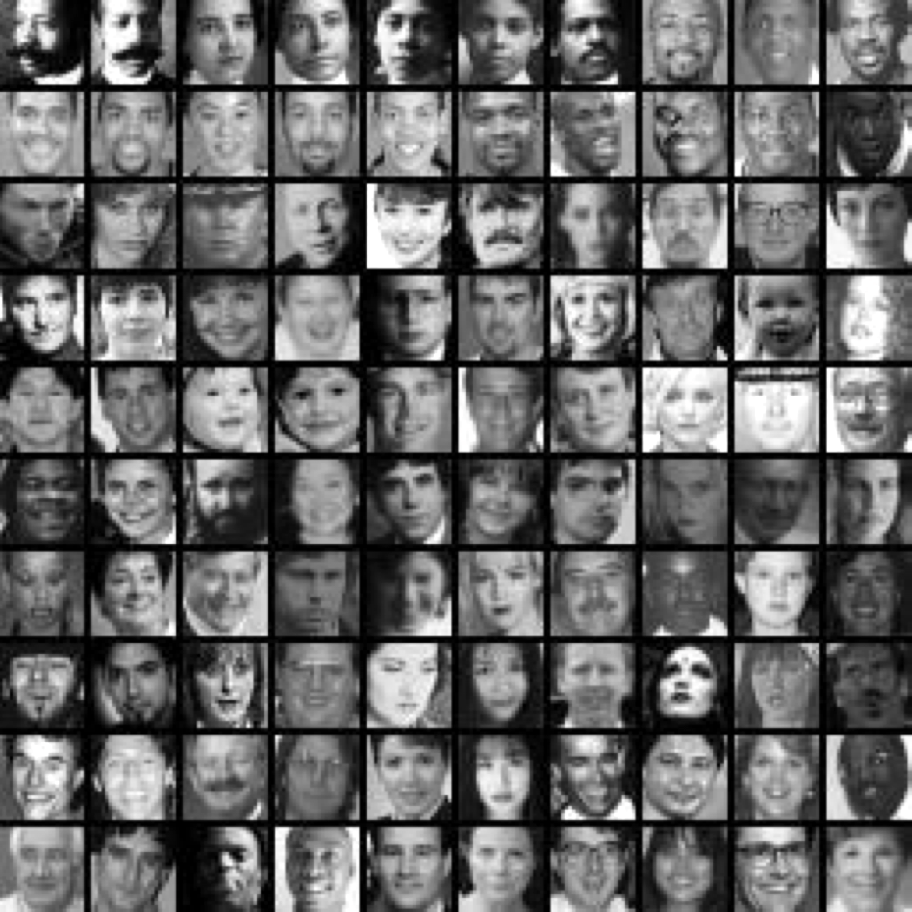
\includegraphics[width=240pt]{chapters/tracking_library_for_the_web/viola_training.png}
  \caption{Example of frontal upright face images used for training \cite{Viola2001}.}
  \label{figure:viola_training}
\end{figure}

A scanning detector was implemented in JavaScript \cite{International2009} and is available on \textit{tracking.js}. The training data used is from OpenCV library \cite{Bradski2000} converted from Extensible Markup Language (XML) \cite{Bray2013} to JavaScript Object Notation (JSON) \cite{Crockford2013}. JSON \cite{Crockford2013} has much superior performance since it's interpreted by JavaScript language \cite{International2009,Crockford2013}. The results of the JavaScript \cite{International2009} implementation can be used in real-time applications, the detector runs at 15 frames per second. For more information about performance see Chapter \ref{cha:evaluation}.

The overall idea of the detection process is that it uses a degenerate decision tree, what Viola and Jones \cite{Viola2001} call ``cascade''. A positive result from the first classifier triggers the evaluation of a second classifier which has also been adjusted to achieve very high detection rates \cite{Viola2001}. A positive result from the second classifier triggers a third classifier, and so on \cite{Viola2001}. The main steps of the scanning algorithm are:

\begin{enumerate}
  \item Create or scale a squared block, initially set to $20\times20$ pixels, by $1.25$ per iteration;
  \item Loop the squared block by $\Delta$ pixels over the image;
  \item For each squared block location, loop the decision tree and evaluate each stage;
  \item A positive result of the stage \cite{Viola2001} triggers the next stage, otherwise stops the stages loop;
  \item If all stages were positively evaluated store that rectangle as a possible face;
  \item Once the decision tree is done, group the overlapping rectangles;
  \item Find the best rectangle of each the group to represent the face. This phase is also known as ``merging phase''.
\end{enumerate}

The final detector is scanned across the image at multiple scales and locations of the image. This process makes sense because the features can be evaluated at any scale with the same cost \cite{Viola2001}. Good results were obtained using a set of scales a factor of $1.25$. Subsequent locations are obtained by shifting the window some number of pixels $\Delta$, for a better accuracy $\Delta=1$ is recommended. We can achieve a significant speedup by setting $\Delta=2$ with only a slight decrease in accuracy, thus this value was set as default value of the JavaScript \cite{International2009} implementation.

Viola and Jones \cite{Viola2001} proposed that for each found possible rectangle representing the face to be partitioned into disjoint subsets data structures. Two detections are in the same subset if their bounding regions overlap \cite{Viola2001}. The corners of the final bounding region are the average of the corners of all detections in the set. In order to perform well on the web, some optimizations were made in the implementation level of the scanning detector. The disjoint set was replaced by an alternative logic that is called ``Minimum Neighbor Area Grouping'' by this thesis. Minimum Neighbor Area Grouping has $O(N^2)$ performance \cite{black2007big} and consists in a loop trough the possible rectangle faces returned by the scanning detector. For each step of the loop compare the current rectangle with all other not yet compared rectangles. If the rectangle area overlaps more than $\eta$ with the compared, by default $\eta=0.5$ (or $50\%$), select the smallest rectangle in area of the comparison. Using the smallest rectangle, guarantees that the best match is much centralized in the face.

For more information about the JavaScript \cite{International2009} implementation, such as evaluation and results, see Chapter \ref{cha:evaluation}.

% subsection contextualization (end)

% section rapid_object_detection (end)

\section{Color Tracking Algorithm} % (fold)
\label{sec:tracking_library_for_the_web:color_tracking_algorithm}

\subsection{Contextualization} % (fold)
\label{sub:tracking_library_for_the_web:color_tracking_algorithm:contextualization}

Colors are part of our lives, they are everywhere in every single object. Being able to use colored objects to control your browser using the user camera is very appealing. For that reason, \textit{training.js} implemented a basic color tracking algorithm that resulted in an real-time frame rate trough a simple and intuitive API.

% subsection contextualization (end)

% section color_tracking_algorithm (end)

% chapter tracking_library_for_the_web (end)
\chapter{Tracking Library for the Web (tracking.js)} % (fold)
\label{cha:tracking_library_for_the_web}

\section{Contextualization} % (fold)
\label{sec:tracking_library_for_the_web:Contextualization}

The desktop platform is the target environment most commonly addressed when developing AR systems. However, depending on the requirements of an AR application, the use of different execution platforms may be necessary. If the system has to be published to several users, the web platform shows to be more adequate, where the application is executed through the Internet in a web browser \cite{Pablo2013}.
The use of markerless tracking, which is based on natural features of the scene, has also been gaining more space on web targeted AR applications for advertising. The media used in this kind of application needs to be as appealing as possible in order to catch consumers' attention. Markerless tracking satisfies this requirement, since the idea of having a real scene augmented with virtual objects without any artificial elements such as markers added to the environment is very attractive \cite{Pablo2013}. In addition, the product being advertised can be tracked and augmented with virtual elements \cite{Pablo2013}.
Browsers are evolving very fast when compared to the the previous decade \cite{Hickson2013}. JavaScript language \cite{International2009,MDN2013} wasn't prepared to handle typed data structures \cite{TypedArray2013} able to manipulate raw binary data safely \cite{Canvas2013}, all the computational complexity required by AR algorithms was too much for that growing environment. Browsers weren't able to capture audio and video \cite{MediaCapture2013,WebRTC2013} natively, without plugin installation \cite{Flash2013}, an essential feature for AR applications. This reality has changed, this involves the use of several modern browser specifications \cite{Hickson2013,WC2006} as well as implementation of different computer vision algorithms and techniques into the browser environment taking advantage of all those modern APIs \cite{Hickson2013,WC2006}.

In this context, this thesis aims to present the implementation and evaluation of a solution regarding tracking techniques for web targeted AR. The available algorithms and techniques can be used for different applications, such as, detect faces, identify objects and colors and track moving objects. The solution is called \textit{tracking.js}. Some optimizations are discussed and implemented on this work in order to achieve good results when compared with similar implementations in compiled languages.

\subsection{Related Work} % (fold)
\label{sub:tracking_library_for_the_web:related_work}

There are not many web based RA solutions available and registered in the literature. The ones available are mainly focused on fiducial markers \cite{Cho1998}, such as FLARToolKit \cite{Yan2011} and JSARToolkit \cite{JSARToolkit2011}, they both are ports of ARToolKit \cite{Hirokazu2002}. ARToolKit is a desktop library which is useful to make vision-based AR applications \cite{Hirokazu2002}. The Metaio company developed Unifeye Viewer \cite{Metaio2009}, a proprietary plug-in for Flash \cite{Flash2013} that allows the utilization of markerless AR applications on the web. In order to run Flash \cite{Flash2013} based applications, the installation of its plugin is required. Third-party plugins, such as Flash \cite{Flash2013}, are in decadency on modern and mobile web browsers, instead JavaScript \cite{International2009} based solutions are preferred, since they can run in any modern browser without requiring any user effort of installing external software. Some smart-phones don't even support Flash \cite{Flash2013} plugin into their browsers, \eg\ Safari for mobile \cite{Safari2013} is one example of a mobile browser that has banned Flash \cite{Flash2013}.

\begin{enumerate}
    \item FLARToolKit: is a port of the well-known ARToolKit \cite{Hirokazu2002} marker tracking library to ActionScript \cite{Flash2013}, which is the language utilized in the development of Flash \cite{Flash2013} applications for the web. This was the first initiative towards AR solutions for the web \cite{Pablo2013}. Using FLARToolKit \cite{Yan2011}, is possible to develop AR applications that runs on client's browser. A marker based AR example for the web, developed for a marketing campaign of General Electric's company using FLARToolKit, is shown on Figure \ref{figure:flartoolkit}.

    \begin{figure}[!htb]
      \centering
      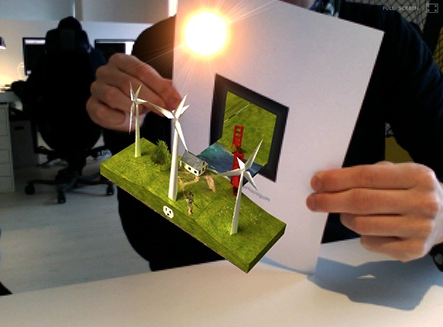
\includegraphics[width=240pt]{chapters/tracking_library_for_the_web/flartoolkit.png}
      \caption{Marker based AR for the web using FLARToolKit.}
      \label{figure:flartoolkit}
    \end{figure}

    \item JSARToolkit: is a JavaScript \cite{International2009} port of FLARToolKit \cite{Yan2011}, operating on canvas images \cite{Canvas2013} and
video element \cite{Hickson2013} contents, provides another marker tracking library. This was the first, open-source, JavaScript \cite{International2009} based, AR solution available for the web. A marker based AR example for the web using JSARToolKit is shown on Figure \ref{figure:jsartoolkit}.

    \begin{figure}[!htb]
      \centering
      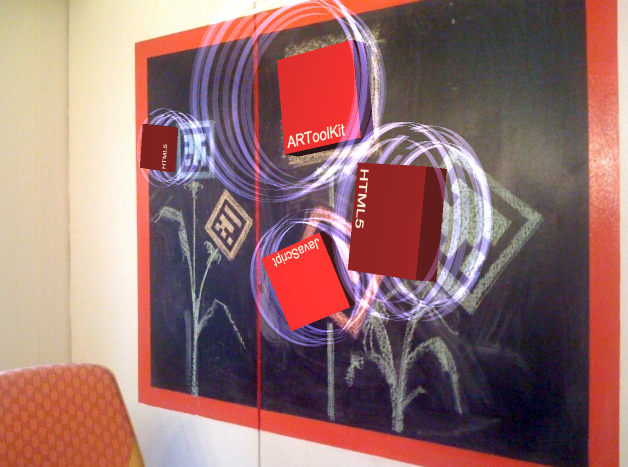
\includegraphics[width=240pt]{chapters/tracking_library_for_the_web/jsartoolkit.png}
      \caption{Marker based AR for the web using JSARToolKit.}
      \label{figure:jsartoolkit}
    \end{figure}

    \item Unifeye Viewer: from Metaio company, offers a robust markerless tracking solution for the web. Unifeye \cite{Metaio2009} also depends on Flash \cite{Flash2013} plugin in order to run on web browsers. A similar example of General Electric's marker based solution, this time markerless based, is shown on Figure \ref{figure:unifeyeviewer}. Note that the 3D image is projected over a magazine cover instead of a fiducial marker \cite{Cho1998}.

    \begin{figure}[!htb]
      \centering
      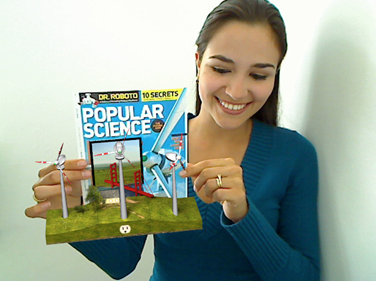
\includegraphics[width=240pt]{chapters/tracking_library_for_the_web/unifeyeviewer.png}
      \caption{Markerless example of image projected over a magazine cover using Unifeye Viewer solution.}
      \label{figure:unifeyeviewer}
    \end{figure}
\end{enumerate}

There is a disadvantage of using marker based AR. Depend on a artificial marker in order to augment the scene with virtual elements is counterintuitive. Commonly, web applications are utilized by novice users that do not have sufficient technical knowledge to perform manual setup, such as print fiducial markers or perform manual initialization for the tracking. FLARToolKit \cite{Yan2011} and JSARToolkit \cite{JSARToolkit2011} are both marker based techniques, using Flash \cite{Flash2013} and JavaScript \cite{International2009}, respectively. FLARToolKit has one more issue which is dependency on Flash \cite{Flash2013} plugin installation. Unifeye Viewer by Metaio, was the only existing solution that provided markerless tracking for the web, although it uses Flash \cite{Flash2013}, excluding it from a potential competitor of \textit{tracking.js}. Markerless tracking techniques do not depend on any artificial marker or advanced user initialization. The space on web targeted AR applications for advertising is gaining more space and the media used in this kind of application needs to be as appealing as possible \cite{Pablo2013}. Making markerless tracking a suitable technique to such applications.

The solution proposed in this thesis, \textit{tracking.js}, provides the first known, open-source, markerless tracking solution for the web that runs entirely in JavaScript \cite{International2009} and HTML5 \cite{Hickson2013}.

% subsection related_work (end)

\subsection{Library Modules} % (fold)
\label{sub:tracking_library_for_the_web:library_modules}

The proposed library is divided in modules in order to allow extension and addition of new features, such as new RA techniques or math utilities. For a better understanding of the library architecture, the current implementation is divided in two packages separating Base from AR classes. Base classes modules are shown in Figure \ref{figure:base_classes} and AR classes in Figure \ref{figure:ar_classes}.

To develop AR applications using only raw JavaScript \cite{International2009} APIs \cite{MDN2013} could be too verbose and complex, \eg\ capturing users' camera and reading its array of pixels. The big amount of steps required for a simple task makes web developers life hard when the goal is to achieve complex implementations. Some level of encapsulation is needed in order to simplify development. The proposed library provides encapsulation for common tasks on the web platform.

The two main available packages splits Base from AR classes. Furthermore, each class of those packages are described. Let's start with the base classes:

\begin{enumerate}
  \item Math: provides common math utilities optimized for the web, such as geometry, linear algebra \cite{Hartley2004} and hamming operations. Typed arrays \cite{TypedArray2013} are used in order to optimize performance, see subsection \ref{sub:basic_concepts:web:javascript_typed_arrays} for more information about typed arrays.
  \item Attribute: allows developers to add attributes to any class through an Attribute interface. The interface adds get and set methods to your class to retrieve and store attribute values, as well as support for change events that can be used to listen for changes in attribute values.
  \item DOMElement: provides a way to create, and manipulate HTML \cite{Hickson2013} DOM nodes \cite{WC2006}. Each DOMElement instance represents an underlying DOM node \cite{WC2006}. In addition to wrapping the basic DOM API \cite{WC2006} and handling cross browser issues, Nodes provide convenient methods for managing styles and subscribing to events.
  \item Canvas: provides an utility class to create, and manipulate HTML5 \cite{Hickson2013} canvas element \cite{Canvas2013}. Each Canvas instance represents an underlying canvas DOM node \cite{Canvas2013}. In addition to wrapping the basic DOM API \cite{WC2006}, also provides methods to extract via \textit{getImageData} method, to loop via \textit{forEach} method, and to set the canvas array of pixels via \textit{setImageData} method.
  \item Video: provides an utility class to create, and manipulate HTML5 \cite{Hickson2013} video element. Each Video instance represents an underlying video DOM node \cite{Canvas2013}. In addition to wrapping the basic DOM API \cite{WC2006}, also provides methods to \textit{play}, \textit{pause} and register tracker algorithms via \textit{track} method. See subsection \ref{sub:basic_concepts:web:audio_and_video} for more information about video element.
  \item VideoCamera: extends all functionalities from Video class with the addition of capturing the user camera via \textit{capture} method. The underlying implementation uses WebRTC \cite{WebRTC2013} and Media Capture and Streams \cite{MediaCapture2013} specifications.
\end{enumerate}

Visual tracking classes includes several computer vision algorithms, such as FAST \cite{RostenFaster2010}, BRIEF \cite{Calonder2010} implementations, homography estimation and others. As the library grows, many other computer vision algorithms are going to be added to the library, such as 3D pose calculation.

\begin{enumerate}
  \item FAST: provides an implementation of Features from Accelerated Segment Test (FAST) \cite{Rosten2010} for features detection via \textit{findCorners(data, threshold)} method, where $data$ is the \textit{ImageData} of the canvas \cite{Canvas2013} frame. It also depends on a $threshold$ argument. The pixel at $p$, see Figure \ref{figure:fast}, is the center of a candidate corner and they are classified if brighter than $p$ by more than the $threshold$.
  \item BRIEF: provides an implementation of Binary Robust Independent Elementary Features (BRIEF) \cite{Calonder2010} for feature extraction via \textit{getDescriptors(data, corners)} method and matching via \textit{match(c1, d1, c2, d2)}, where $data$ is an \textit{ImageData}, and $c1$ and $c2$ are the found corners array return by \textit{FAST.findCorners} method and $d1$ and $d2$ are feature descriptors array return by \textit{BRIEF.getDescriptors} method.
  \item RANSAC: provides an interface used to achieve robust estimation method for homographies and camera pose. There are two available estimation methods implemented that inherits from RANSAC \cite{Hartley2004}, Homography and Pose.
  \item Homography: provides an API to estimate a homography matrix $H$ between images by finding feature correspondences in those images.
  \item Pose: TODO.
  \item ViolaJones: TODO.
  \item Color: TODO.
\end{enumerate}

\begin{figure}[!htb]
    % \tikzumlset{font=\scriptsize}
    \begin{tikzpicture}
        \begin{umlpackage}{Base classes}

            \umlclass[y=-50pt,x=190pt]{Math}{}{
              createIdentityMatrix(size) : Matrix\\
              distance(x1, y1, x2, y2) : Number\\
              getDeterminant(Matrix) : Number\\
              getInverse(Matrix) : Matrix\\
              hammingDistance(n1, n2) : Number\\
              hammingWeight(number) : Number\\
              ...
            }

            \umlclass{Attribute}{}{
              get(name) : Object\\
              set(name, value) : void \\
            }

            \umlclass[y=-100pt]{DOMElement}{
              width : Number\\
              height : Number\\
              visible : boolean\\
            }{
              show() : void\\
              hide() : void \\
            }

            \umlclass[y=-220pt,x=180pt]{Canvas}{
              context : Object
            }{
              forEach(data, callback) : void\\
              getImageData(x, y, width, height) : ImageData \\
              setImageData(data, x, y) : void\\
            }

            \umlclass[y=-335pt]{Video}{}{
              play() : void\\
              pause() : void\\
              track(tracker) : void \\
              getVideoCanvasImageData(x, y, width, height) : ImageData \\
            }

            \umlclass[y=-335pt,x=220pt]{VideoCamera}{}{
              capture() : void \\
            }

        \end{umlpackage}

        \umlinherit[geometry=-|]{DOMElement}{Attribute}
        \umlinherit[geometry=-|]{Canvas}{DOMElement}
        \umlinherit[geometry=-|]{Video}{DOMElement}
        \umlinherit[geometry=|-]{VideoCamera}{Video}
    \end{tikzpicture}
    \caption{Base classes of tracking.js library.}
    \label{figure:base_classes}
\end{figure}

\begin{figure}[!htb]
    % \tikzumlset{font=\scriptsize}
    \begin{tikzpicture}
        \begin{umlpackage}{Visual tracking classes}

            \umlclass{FAST}{}{
              findCorners(data, threshold) : Array\\
            }

            \umlclass[y=-70pt]{BRIEF}{}{
              getDescriptors(data, corners) : Array\\
              match(c1, d1, c2, d2) : Array\\
            }

            \umlclass[y=-150pt]{ViolaJones}{}{
              find() : Array\\
              evalStage() : boolean\\
            }

            \umlclass[y=-225pt]{Color}{}{
              find() : Array\\
            }

            \umlclass[x=200pt]{RANSAC}{}{
              find(matches) : void\\
              score() : Number\\
            }

            \umlclass[y=-90pt,x=200pt]{Homography}{}{
                score(H, matches) : Number\\
            }

            \umlclass[y=-170pt,x=200pt]{Pose}{}{
              find(points2d, points3d) : void\\
            }

        \end{umlpackage}

        \umlinherit[geometry=-|]{Homography}{RANSAC}
        \umlinherit[geometry=-|]{Pose}{RANSAC}
    \end{tikzpicture}
    \caption{Visual tracking classes of tracking.js library.}
    \label{figure:ar_classes}
\end{figure}

\newpage

% subsection library_modules (end)

% section contextualization (end)

\section{Markerless Tracking Algorithm} % (fold)
\label{sec:tracking_library_for_the_web:marker_less_tracking_algorithm}

\subsection{Contextualization} % (fold)
\label{sub:tracking_library_for_the_web:marker_less_tracking_algorithm:contextualization}

Lorem ipsum dolor sit amet, consectetur adipisicing elit.

% subsection contextualization (end)

\subsection{Feature Detector} % (fold)
\label{sub:tracking_library_for_the_web:marker_less_tracking_algorithm:feature_detector}

This technique relies on matching individual features across images and are therefore easy to increase robustness against partial occlusions or matching errors. Illumination invariance is also simple to achieve. Feature points detection is used as the first step of many vision tasks such as tracking, localization, image matching and recognition. In this article we call ``feature'' or ``keypoint'' to refer to a point of interest in two dimensions.

For each frame, the object features are matched by localizing feature templates in search windows around hypothesized locations \cite{Lepetit2005}. The method to extract feature points suggested in Features from Accelerated Segment Test (FAST) \cite{Rosten2010}. FAST \cite{RostenFaster2010} hypothesizes the matches using corner detection. A large number of corner detectors exist in the literature. However, we have a strong interest in real time frame rate applications which computational resources are required requisites. The approach proposed by FAST \cite{RostenFaster2010} allows the detector to produce a suite of high-speed detectors which we currently use for real-time tracking and AR label placement \cite{Calonder2010}. In particular, it is still true that when processing live video streams at full frame rate, existing feature detectors leave little if any time for further processing, even despite the consequences of Moore's Law \cite{Rosten2010}.

To show that speed can been obtained without necessarily sacrificing the quality of the feature detector, in Chapter \ref{cha:evaluation}, we compare our detector, to a variety of well-known detectors. A number of the detectors described below compute a corner response, (1) Edge based corner detectors, corresponds to the boundary between two regions; (2) Gray level derivative based detectors, the assumption that corners exist along edges is an inadequate model for patches of texture and point like features, and is difficult to use at junctions. Therefore a large number of detectors operate directly on gray level images without requiring edge detection; and (3) Direct gray level detectors, Another major class of corner detectors work by examining a small patch of an image to see if it ``looks'' like a corner \cite{Rosten2010}.

The thesis choice was (3) Direct gray level detectors. It works by testing a small patch of an image to see if it could be a corner. The detector is evaluated using a circle surrounding the candidate pixel, the test is based on whether the concentric contiguous arcs around the pixel are significantly different from the central pixel $p$ \cite{Rosten2010}. To classify $p$ as a corner should exists a set of $n$ contiguous pixels in the circle which are all brighter than the intensity of the candidate pixel $I_{p} + t$ (threshold), or all darker than $I_{p} - t$ \cite{Rosten2010}.

The number of contiguous tested pixels could vary accordingly \cite{Rosten2010}, being more common to be FAST-$12$ or FAST-$9$. Empirically, FAST-$9$ showed to have a good repeatability and a better efficiency on the web. The repeatability of found feature points is also important because determines whether the technique is useful in a real-world application.

This detector in itself exhibits high performance, but there are several weaknesses: (1) This high-speed test does not reject as many candidates; (2) The efficiency of the detector will depend on the ordering of the questions and the distribution of corner appearances; and (3) Multiple features are detected adjacent to one another \cite{Rosten2010}.

On Figure \ref{figure:fast}, the highlighted squares are the pixels used in the corner detection. The pixel at $p$ is the central pixel. The arc is indicating that the dashed line passes through FAST-$n$, let $n$ be $9$ or $12$ contiguous pixels which are brighter or darker than $p$ \cite{Rosten2010}.

\begin{figure}[!htb]
  \centering
  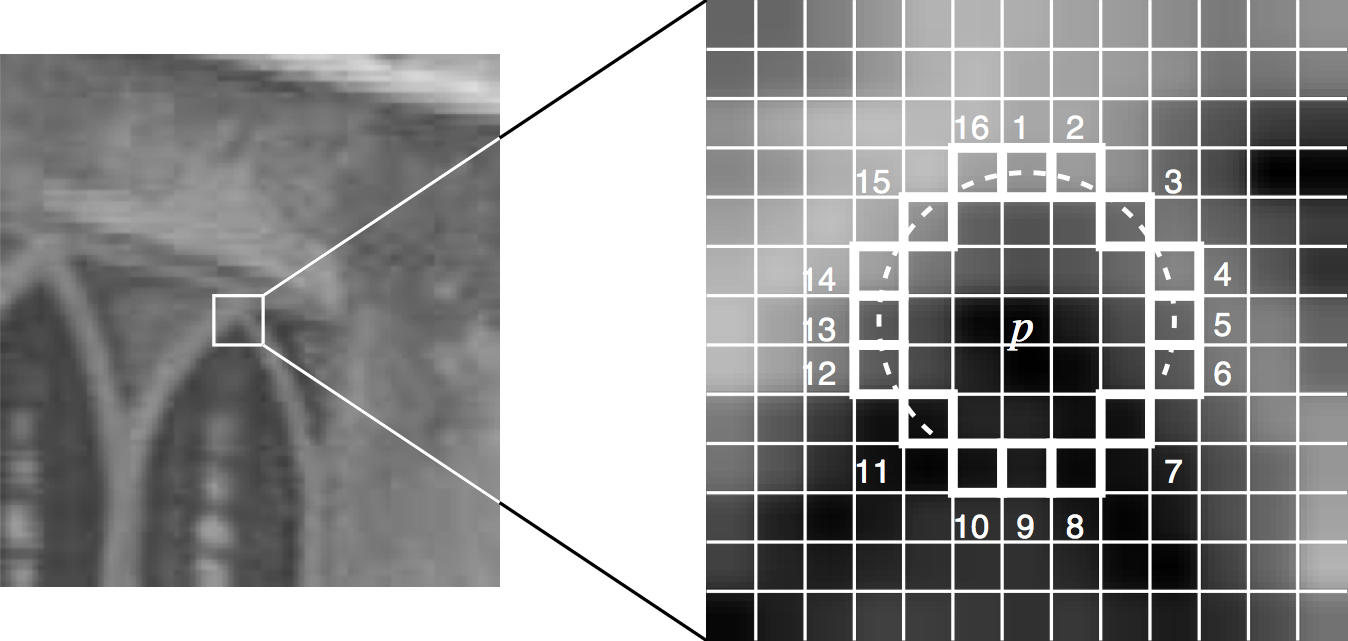
\includegraphics[width=380pt]{chapters/tracking_library_for_the_web/fast.png}
  \caption{Point segment test corner detection in an image patch \cite{Glass2013}.}
  \label{figure:fast}
\end{figure}

% subsection feature_detector (end)

\subsection{Feature Extractors} % (fold)
\label{sub:tracking_library_for_the_web:marker_less_tracking_algorithm:feature_extractors}

To estimate motion, one can then match sets of features \{$m_{i}$\} and \{$m'_{j}$\} extracted from two images taken from similar, and often successive, viewpoints. A classical procedure \cite{Calonder2010} runs as follows. For each point \{$m_{i}$\} in the first image, search in a region of the second image around location \{$m_{i}$\} for point \{$m'_{j}$\}. The search is based on the similarity of the local image windows, also knowns as kernel windows, centered on the points, which strongly characterizes the points when the images are sufficiently close \cite{Lepetit2005}.

\begin{figure}[!htb]
  \centering
  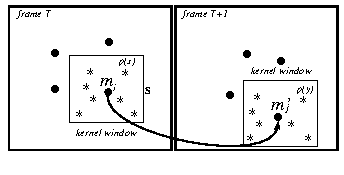
\includegraphics[width=\linewidth]{chapters/tracking_library_for_the_web/BRIEF.pdf}
  \caption{BRIEF \cite{Lepetit2005} feature extractor.}
  \label{figure:BRIEF}
\end{figure}

The feature matching used in the case studies performed in this work search for correspondent points in the current frame. Only points that are highly descriptive invariant features, called keypoints, are tested. Those keypoints were detected using FAST \cite{Rosten2010} in Section \ref{sub:tracking_library_for_the_web:marker_less_tracking_algorithm:feature_detector}. After the keypoints are detected they need to be described and the respective matching point should be found. Since web and handled devices have limited computational power having local descriptors that are fast to compute, to match and being memory efficient are important aspects, for that reason, was used an efficient method called Binary Robust Independent Elementary Features (BRIEF) \cite{Calonder2010}.

To generate the binary string for each key-point found in the smoothed frame, the individual bits are obtained by comparing the intensities of pairs of points, $(\textbf{p}; x, y)$, represented by $\ast$ symbol on Figure \ref{figure:BRIEF}, along the kernel window centered on each key-point without requiring a training phase.
Empirically, this technique shows that $256$ or even $128$ bits \cite{Calonder2010}, often suffice to obtain very good matching results. The best spatial arrangement of the tested (\textbf{x}, \textbf{y})-pairs of points are reach when selected based on an isotropic Gaussian distribution \cite{Calonder2010}. To compute the Gaussian distribution can be time consuming. As an optimization proposed by this article, the Gaussian distribution could be simply replaced by a random function due to its random characteristics.

To generate the binary strings is defined test $\tau$ on patch \textbf{p} of size \textbf{S $\times$ S} as

$$\tau(\textbf{p}; x, y) :=
\begin{cases}
  1 &\mbox{if}\quad \textbf{p(x)} < \textbf{p(y)},\\
  0 &\mbox{otherwise}
\end{cases}$$

where \textbf{p(x)} is the pixel intensity. The set of binary tests is defined by the $n_{d}$ (\textbf{x}, \textbf{y})-location pairs uniquely chosen during the initialization. The $n_{d}$-dimensional bit-string is our BRIEF descriptor for each key-point

$$f_{n_{d}}(\textbf{p}) := \sum_{1 \le i \le n_{d}} 2^{i-1} \tau(\textbf{p}; x, y).$$

In \cite{Calonder2010}, $n_{d}= 128, 256, 512$ were used in the tests and any of those values yield good compromises between speed, storage efficiency, and recognition rate. In this article, $n_{d}= 128$ was used, since it presented good matching results and performance. The number of bytes required to store the descriptor can be calculated by $k = n_{d}/8$, proving that BRIEF is also a memory-efficient method. Detailed results can be found in Chapter \ref{cha:evaluation}.

Once each keypoint is described with its binary string \cite{Calonder2010}, they need to be compared with the closest matching point. Distance metric is critical to the performance of intrusion detection systems. Thus using binary strings reduces the size of the descriptor and provides an interesting data structure that is fast to operate with whose similarity can be measured by the Hamming distance which, on desktop implementations, the computation time could be driven almost to zero using the POPCNT instruction from SSE4.2 \cite{Intel2007}. Only the latest Intel Core i7 CPUs support this instruction.

The Hamming distance is an important step on feature matching, it provides a fast and memory-efficient way to calculate distance between binary strings. Given two image patches $x$ and $y$, denote their binary descriptors as $b(x) \in \{0,1\}^n$ and $b(y) \in \{0,1\}^n$ respectively. Then their Hamming distance is computed by:

$$Ham(x, y)=\sum_{i=1}^{n}b_i(x)\otimes b_i(y)$$

In which $n$ is the dimension of binary descriptor and stands for bitwise XOR operation. According to the definition of Hamming distance, all the elements of a binary descriptor contribute equally to the distance. From the hamming distance, the Hamming weight can be calculated. It is used to find the best feature point match. Here, is generalized the Hamming distance to the weighted Hamming:

$$WHam(x, y)=\sum_{i=1}^{n}w_i(b_i(x)\otimes b_i(y))$$

Where $w_i$ is the weight of the $i$th element. The goal is to learn $w_i,i=1,2\cdots,n$ for the binary descriptor (BRIEF) based on a set of feature points. By assigning different weights to binary codes, what we expect is to obtain a distance space in which the distances of matching patches are less than those of non-matching patches.

% subsection feature_extractors (end)

\subsection{Homography Estimation} % (fold)
\label{sub:tracking_library_for_the_web:marker_less_tracking_algorithm:homography_estimation}

Typically, homographies are estimated between images by finding feature correspondences in those images. A 2D point $(x,y)$ in an image can be represented as a 3D vector $\textbf{x} = (x_1, x_2, x_3)$ where $x = \frac{x_1}{x_3}$ and $y = \frac{x_2}{x_3}$ \cite{Homography2009}. This is called the homogeneous representation of a point and it lies on the projective plane $P^2$. A homography is an invertible mapping of points and lines on the projective plane $P^2$. Hartley and Zisserman \cite{Hartley2004} provide the specific definition that a homography is a mapping from $P^2$ → $P^2$ is a projectivity if and only if there exists a non-singular $3\times3$ matrix $H$ such that for any point in $P^2$ represented by vector $\textbf{x}$ it is true that its mapped point equals $H\textbf{x}$. It should be noted that $H$ can be changed by multiplying by an arbitrary non-zero constant without altering the projective transformation. Thus $H$ is considered a homogeneous matrix and only has $8$ degrees of freedom even though it contains $9$ elements.

The method chosen to solve the homography estimation was the Direct Linear Transformation (DLT) \cite{Impa2009,Hartley2004} algorithm. The DLT algorithm is a simple algorithm used to solve for the homography matrix $H$ given a sufficient set of point correspondences \cite{Homography2009}.

Since we are working in homogeneous coordinates, the relationship between two corresponding points $\textbf{x}$ and $\textbf{x'}$ can be re-written as \cite{Homography2009}:

$$c\begin{pmatrix}u\\ v\\ 1\\\end{pmatrix} = H\begin{pmatrix}x\\ y\\ 1\\\end{pmatrix} \;\; \forall \;\; H=\begin{pmatrix}h1 & h2 & h3\\ h4 & h5 & h6\\ h7 & h8 & h9\\\end{pmatrix},$$

where $c$ is any non-zero constant, $(\; u \; v \; 1 \;)^T$ represents $\textbf{x'}$, $(\; x \; y \; 1 \;)^T$ represents $\textbf{x}$. Dividing the first row of equation (2.1) by the third row and the second row by the third row we get the following two equations \cite{Homography2009}:

\begin{equation}
\label{eq:homography1}
-h1x-h2y-h3 +(h7x+h8y+h9)u=0
\end{equation}
\begin{equation}
\label{eq:homography2}
-h4x-h5y-h6 +(h7x+h8y+h9)u=0
\end{equation}

Equations (\ref{eq:homography1}) and (\ref{eq:homography2}) can be written in matrix form as $A_i\textbf{h}=0$. Where,

$$A_i=\begin{pmatrix}-x & -y & -1 & 0 & 0 & 0 & ux & uy & u\\0 & 0 & 0 & -x & -y & -1 & vx & vy & v\end{pmatrix}$$

and

$$\textbf{h}=\begin{pmatrix}h1 & h2 & h3 & h4 & h5 & h6 & h7 & h8 & h9\end{pmatrix}.$$

Since each point correspondence provides $2$ equations, $4$ correspondences are sufficient to solve for the $8$ degrees of freedom of $H$. JavaScript typed arrays, defined in Section \ref{sub:basic_concepts:web:javascript_typed_arrays}, were used in the homography estimation implementation for better performance results.

% subsection homography_estimation (end)

\subsection{Random Sample Consensus (RANSAC)} % (fold)
\label{sub:tracking_library_for_the_web:marker_less_tracking_algorithm:ransac}

RANSAC (Random Sample Consensus) \cite{Hartley2004} is the most commonly used robust estimation method for homographies according to \cite{Homography2009}. The idea of the algorithm is pretty simple; For a number of iterations, a random sample of $4$ correspondences is selected and a homography $H$ is computed from those four correspondences. Each other correspondence is then classified as an inlier or outlier depending on its concurrence with $H$. After all of the iterations are done, the iteration that contained the largest number of inliers is selected. $H$ can then be recomputed from all of the correspondences that were consider as inliers in that iteration \cite{Homography2009}.

One important step when applying the RANSAC algorithm described above is to decide how to classify correspondences as inliers or outliers. In the implementation for the web only assign the geometric distance \cite{Homography2009} threshold, $t$, between $\textbf{x'}$ and $H\textbf{x}$ was enough. Hartley and Zisserman \cite{Hartley2004} provides more details about RANSAC.

Another issue is to decide how many iterations to run the algorithm, it's not required to try every combination of 4 correspondences. The goal becomes to determine the number of iterations, $N$, that ensures with a probability $p$ that at least one of the random samples will be free from outliers. $N=100$ was used on the web implementation.

% subsection ransac (end)

% section marker_less_tracking_algorithm (end)

\section{Rapid Object Detection (Viola Jones)} % (fold)
\label{sec:tracking_library_for_the_web:rapid_object_detection}

\subsection{Contextualization} % (fold)
\label{sub:tracking_library_for_the_web:rapid_object_detection:contextualization}

Rapid Object Detection \cite{Viola2001} technique, much known as Viola Jones \cite{Viola2001}, brings together new algorithms and insights to construct a library for robust and extremely rapid object detection. What has motivated this technique to be added to \textit{tracking.js} library was the task of face detection. Surprisingly, the algorithm became robust enough to detect any training data \cite{Viola2001}, not only for faces. Currently, \textit{tracking.js} supports, face, eyes, upper body and palm detection.

In order to scan faces, eyes or palm from images, a training phase is required. The training phase generate cascading stages. The cascade are constructed by training classifiers using AdaBoost \cite{Viola2001} and then adjusting the threshold to minimize false negatives. OpenCV library \cite{Bradski2000} has some open-source training data, therefore doubling efforts on training is unnecessary, \ie\ the face training set consisted of 4916 faces, extracted from images downloaded during a random crawl of the world wide web \cite{Viola2001}. Those faces were scaled and aligned to a base resolution of $24$ by $24$ pixels \cite{Viola2001}, see Figure \ref{figure:viola_training}. Training is not the focus of this work, the algorithm to scan the faces is. The training data itself is useless if a Scanning Detector \cite{Viola2001} is not available, the scanning is what makes the rapid object detection.

\begin{figure}[!htb]
  \centering
  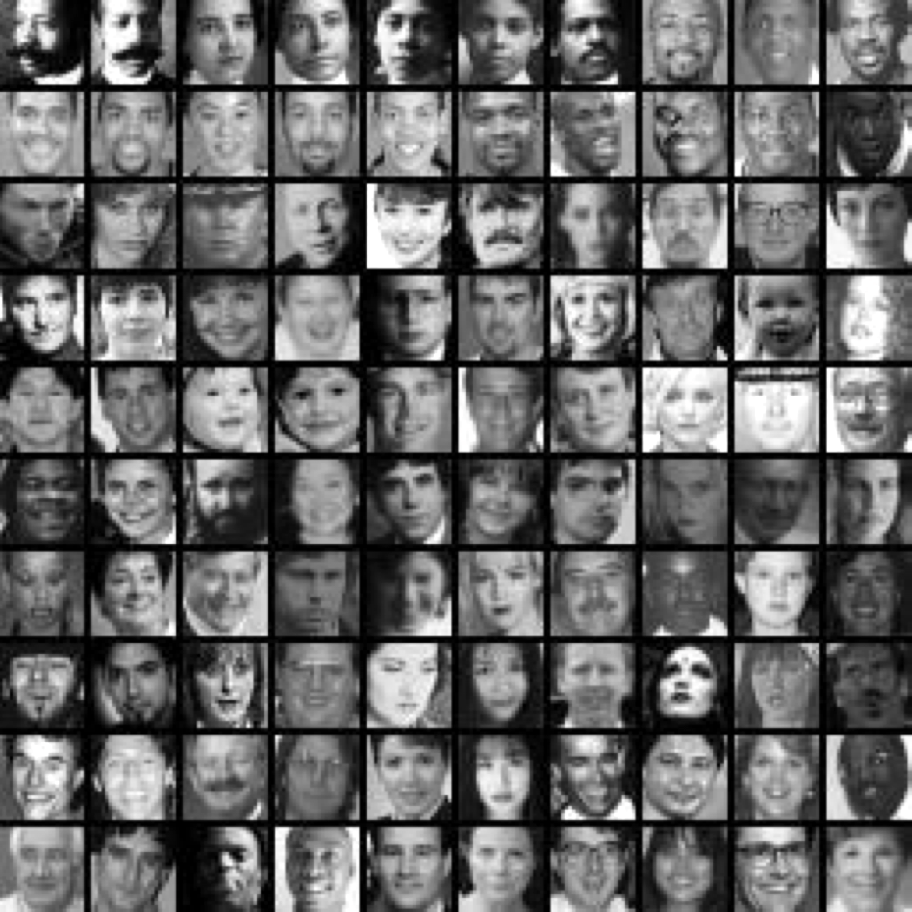
\includegraphics[width=240pt]{chapters/tracking_library_for_the_web/viola_training.png}
  \caption{Example of frontal upright face images used for training \cite{Viola2001}.}
  \label{figure:viola_training}
\end{figure}

A scanning detector was implemented in JavaScript \cite{International2009} and is available on \textit{tracking.js}. The training data used is from OpenCV library \cite{Bradski2000} converted from Extensible Markup Language (XML) \cite{Bray2013} to JavaScript Object Notation (JSON) \cite{Crockford2013}. JSON \cite{Crockford2013} has much superior performance since it's interpreted by JavaScript language \cite{International2009,Crockford2013}. The results of the JavaScript \cite{International2009} implementation can be used in real-time applications, the detector runs at 15 frames per second. For more information about performance see Chapter \ref{cha:evaluation}.

The overall idea of the detection process is that it uses a degenerate decision tree, what Viola and Jones \cite{Viola2001} call ``cascade''. A positive result from the first classifier triggers the evaluation of a second classifier which has also been adjusted to achieve very high detection rates \cite{Viola2001}. A positive result from the second classifier triggers a third classifier, and so on \cite{Viola2001}. The main steps of the scanning algorithm are:

\begin{enumerate}
  \item Create or scale a squared block, initially set to $20\times20$ pixels, by $1.25$ per iteration;
  \item Loop the squared block by $\Delta$ pixels over the image;
  \item For each squared block location, loop the decision tree and evaluate each stage;
  \item A positive result of the stage \cite{Viola2001} triggers the next stage, otherwise stops the stages loop;
  \item If all stages were positively evaluated store that rectangle as a possible face;
  \item Once the decision tree is done, group the overlapping rectangles;
  \item Find the best rectangle of each the group to represent the face. This phase is also known as ``merging phase''.
\end{enumerate}

The final detector is scanned across the image at multiple scales and locations of the image. This process makes sense because the features can be evaluated at any scale with the same cost \cite{Viola2001}. Good results were obtained using a set of scales a factor of $1.25$. Subsequent locations are obtained by shifting the window some number of pixels $\Delta$, for a better accuracy $\Delta=1$ is recommended. We can achieve a significant speedup by setting $\Delta=2$ with only a slight decrease in accuracy, thus this value was set as default value of the JavaScript \cite{International2009} implementation.

Viola and Jones \cite{Viola2001} proposed that for each found possible rectangle representing the face to be partitioned into disjoint subsets data structures. Two detections are in the same subset if their bounding regions overlap \cite{Viola2001}. The corners of the final bounding region are the average of the corners of all detections in the set. In order to perform well on the web, some optimizations were made in the implementation level of the scanning detector. The disjoint set was replaced by an alternative logic that is called ``Minimum Neighbor Area Grouping'' by this thesis. Minimum Neighbor Area Grouping has $O(N^2)$ performance \cite{black2007big} and consists in a loop trough the possible rectangle faces returned by the scanning detector. For each step of the loop compare the current rectangle with all other not yet compared rectangles. If the rectangle area overlaps more than $\eta$ with the compared, by default $\eta=0.5$ (or $50\%$), select the smallest rectangle in area of the comparison. Using the smallest rectangle, guarantees that the best match is much centralized in the face.

For more information about the JavaScript \cite{International2009} implementation, such as evaluation and results, see Chapter \ref{cha:evaluation}.

% subsection contextualization (end)

% section rapid_object_detection (end)

\section{Color Tracking Algorithm} % (fold)
\label{sec:tracking_library_for_the_web:color_tracking_algorithm}

\subsection{Contextualization} % (fold)
\label{sub:tracking_library_for_the_web:color_tracking_algorithm:contextualization}

Colors are part of our lives, they are everywhere in every single object. Being able to use colored objects to control your browser using the user camera is very appealing. For that reason, \textit{training.js} implemented a basic color tracking algorithm that resulted in an real-time frame rate trough a simple and intuitive API.

% subsection contextualization (end)

% section color_tracking_algorithm (end)

% chapter tracking_library_for_the_web (end)
\chapter{Tracking Library for the Web (tracking.js)} % (fold)
\label{cha:tracking_library_for_the_web}

\section{Contextualization} % (fold)
\label{sec:tracking_library_for_the_web:Contextualization}

The desktop platform is the target environment most commonly addressed when developing AR systems. However, depending on the requirements of an AR application, the use of different execution platforms may be necessary. If the system has to be published to several users, the web platform shows to be more adequate, where the application is executed through the Internet in a web browser \cite{Pablo2013}.
The use of markerless tracking, which is based on natural features of the scene, has also been gaining more space on web targeted AR applications for advertising. The media used in this kind of application needs to be as appealing as possible in order to catch consumers' attention. Markerless tracking satisfies this requirement, since the idea of having a real scene augmented with virtual objects without any artificial elements such as markers added to the environment is very attractive \cite{Pablo2013}. In addition, the product being advertised can be tracked and augmented with virtual elements \cite{Pablo2013}.
Browsers are evolving very fast when compared to the the previous decade \cite{Hickson2013}. JavaScript language \cite{International2009,MDN2013} wasn't prepared to handle typed data structures \cite{TypedArray2013} able to manipulate raw binary data safely \cite{Canvas2013}, all the computational complexity required by AR algorithms was too much for that growing environment. Browsers weren't able to capture audio and video \cite{MediaCapture2013,WebRTC2013} natively, without plugin installation \cite{Flash2013}, an essential feature for AR applications. This reality has changed, this involves the use of several modern browser specifications \cite{Hickson2013,WC2006} as well as implementation of different computer vision algorithms and techniques into the browser environment taking advantage of all those modern APIs \cite{Hickson2013,WC2006}.

In this context, this thesis aims to present the implementation and evaluation of a solution regarding tracking techniques for web targeted AR. The available algorithms and techniques can be used for different applications, such as, detect faces, identify objects and colors and track moving objects. The solution is called \textit{tracking.js}. Some optimizations are discussed and implemented on this work in order to achieve good results when compared with similar implementations in compiled languages.

\subsection{Related Work} % (fold)
\label{sub:tracking_library_for_the_web:related_work}

There are not many web based RA solutions available and registered in the literature. The ones available are mainly focused on fiducial markers \cite{Cho1998}, such as FLARToolKit \cite{Yan2011} and JSARToolkit \cite{JSARToolkit2011}, they both are ports of ARToolKit \cite{Hirokazu2002}. ARToolKit is a desktop library which is useful to make vision-based AR applications \cite{Hirokazu2002}. The Metaio company developed Unifeye Viewer \cite{Metaio2009}, a proprietary plug-in for Flash \cite{Flash2013} that allows the utilization of markerless AR applications on the web. In order to run Flash \cite{Flash2013} based applications, the installation of its plugin is required. Third-party plugins, such as Flash \cite{Flash2013}, are in decadency on modern and mobile web browsers, instead JavaScript \cite{International2009} based solutions are preferred, since they can run in any modern browser without requiring any user effort of installing external software. Some smart-phones don't even support Flash \cite{Flash2013} plugin into their browsers, \eg\ Safari for mobile \cite{Safari2013} is one example of a mobile browser that has banned Flash \cite{Flash2013}.

\begin{enumerate}
    \item FLARToolKit: is a port of the well-known ARToolKit \cite{Hirokazu2002} marker tracking library to ActionScript \cite{Flash2013}, which is the language utilized in the development of Flash \cite{Flash2013} applications for the web. This was the first initiative towards AR solutions for the web \cite{Pablo2013}. Using FLARToolKit \cite{Yan2011}, is possible to develop AR applications that runs on client's browser. A marker based AR example for the web, developed for a marketing campaign of General Electric's company using FLARToolKit, is shown on Figure \ref{figure:flartoolkit}.

    \begin{figure}[!htb]
      \centering
      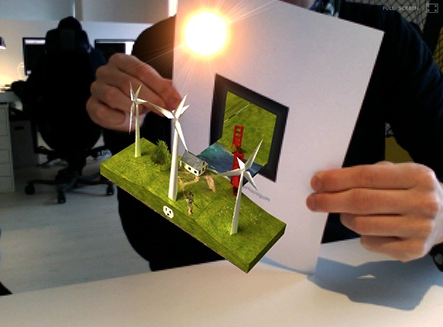
\includegraphics[width=240pt]{chapters/tracking_library_for_the_web/flartoolkit.png}
      \caption{Marker based AR for the web using FLARToolKit.}
      \label{figure:flartoolkit}
    \end{figure}

    \item JSARToolkit: is a JavaScript \cite{International2009} port of FLARToolKit \cite{Yan2011}, operating on canvas images \cite{Canvas2013} and
video element \cite{Hickson2013} contents, provides another marker tracking library. This was the first, open-source, JavaScript \cite{International2009} based, AR solution available for the web. A marker based AR example for the web using JSARToolKit is shown on Figure \ref{figure:jsartoolkit}.

    \begin{figure}[!htb]
      \centering
      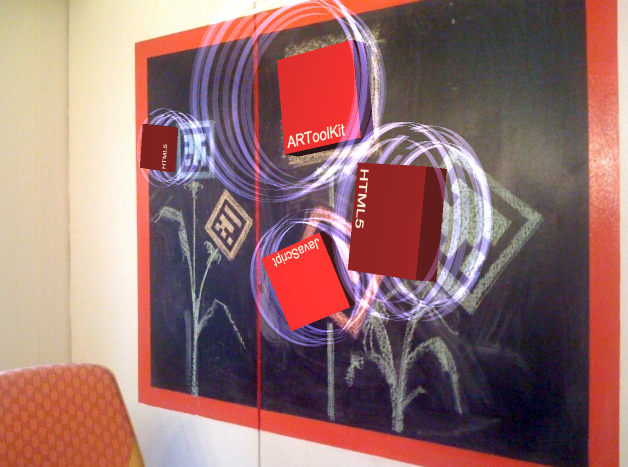
\includegraphics[width=240pt]{chapters/tracking_library_for_the_web/jsartoolkit.png}
      \caption{Marker based AR for the web using JSARToolKit.}
      \label{figure:jsartoolkit}
    \end{figure}

    \item Unifeye Viewer: from Metaio company, offers a robust markerless tracking solution for the web. Unifeye \cite{Metaio2009} also depends on Flash \cite{Flash2013} plugin in order to run on web browsers. A similar example of General Electric's marker based solution, this time markerless based, is shown on Figure \ref{figure:unifeyeviewer}. Note that the 3D image is projected over a magazine cover instead of a fiducial marker \cite{Cho1998}.

    \begin{figure}[!htb]
      \centering
      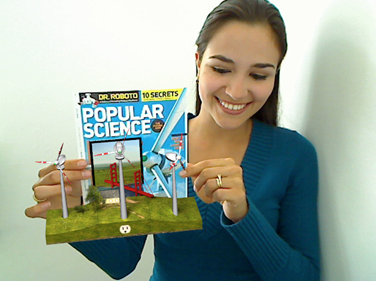
\includegraphics[width=240pt]{chapters/tracking_library_for_the_web/unifeyeviewer.png}
      \caption{Markerless example of image projected over a magazine cover using Unifeye Viewer solution.}
      \label{figure:unifeyeviewer}
    \end{figure}
\end{enumerate}

There is a disadvantage of using marker based AR. Depend on a artificial marker in order to augment the scene with virtual elements is counterintuitive. Commonly, web applications are utilized by novice users that do not have sufficient technical knowledge to perform manual setup, such as print fiducial markers or perform manual initialization for the tracking. FLARToolKit \cite{Yan2011} and JSARToolkit \cite{JSARToolkit2011} are both marker based techniques, using Flash \cite{Flash2013} and JavaScript \cite{International2009}, respectively. FLARToolKit has one more issue which is dependency on Flash \cite{Flash2013} plugin installation. Unifeye Viewer by Metaio, was the only existing solution that provided markerless tracking for the web, although it uses Flash \cite{Flash2013}, excluding it from a potential competitor of \textit{tracking.js}. Markerless tracking techniques do not depend on any artificial marker or advanced user initialization. The space on web targeted AR applications for advertising is gaining more space and the media used in this kind of application needs to be as appealing as possible \cite{Pablo2013}. Making markerless tracking a suitable technique to such applications.

The solution proposed in this thesis, \textit{tracking.js}, provides the first known, open-source, markerless tracking solution for the web that runs entirely in JavaScript \cite{International2009} and HTML5 \cite{Hickson2013}.

% subsection related_work (end)

\subsection{Library Modules} % (fold)
\label{sub:tracking_library_for_the_web:library_modules}

The proposed library is divided in modules in order to allow extension and addition of new features, such as new RA techniques or math utilities. For a better understanding of the library architecture, the current implementation is divided in two packages separating Base from AR classes. Base classes modules are shown in Figure \ref{figure:base_classes} and AR classes in Figure \ref{figure:ar_classes}.

To develop AR applications using only raw JavaScript \cite{International2009} APIs \cite{MDN2013} could be too verbose and complex, \eg\ capturing users' camera and reading its array of pixels. The big amount of steps required for a simple task makes web developers life hard when the goal is to achieve complex implementations. Some level of encapsulation is needed in order to simplify development. The proposed library provides encapsulation for common tasks on the web platform.

The two main available packages splits Base from AR classes. Furthermore, each class of those packages are described. Let's start with the base classes:

\begin{enumerate}
  \item Math: provides common math utilities optimized for the web, such as geometry, linear algebra \cite{Hartley2004} and hamming operations. Typed arrays \cite{TypedArray2013} are used in order to optimize performance, see subsection \ref{sub:basic_concepts:web:javascript_typed_arrays} for more information about typed arrays.
  \item Attribute: allows developers to add attributes to any class through an Attribute interface. The interface adds get and set methods to your class to retrieve and store attribute values, as well as support for change events that can be used to listen for changes in attribute values.
  \item DOMElement: provides a way to create, and manipulate HTML \cite{Hickson2013} DOM nodes \cite{WC2006}. Each DOMElement instance represents an underlying DOM node \cite{WC2006}. In addition to wrapping the basic DOM API \cite{WC2006} and handling cross browser issues, Nodes provide convenient methods for managing styles and subscribing to events.
  \item Canvas: provides an utility class to create, and manipulate HTML5 \cite{Hickson2013} canvas element \cite{Canvas2013}. Each Canvas instance represents an underlying canvas DOM node \cite{Canvas2013}. In addition to wrapping the basic DOM API \cite{WC2006}, also provides methods to extract via \textit{getImageData} method, to loop via \textit{forEach} method, and to set the canvas array of pixels via \textit{setImageData} method.
  \item Video: provides an utility class to create, and manipulate HTML5 \cite{Hickson2013} video element. Each Video instance represents an underlying video DOM node \cite{Canvas2013}. In addition to wrapping the basic DOM API \cite{WC2006}, also provides methods to \textit{play}, \textit{pause} and register tracker algorithms via \textit{track} method. See subsection \ref{sub:basic_concepts:web:audio_and_video} for more information about video element.
  \item VideoCamera: extends all functionalities from Video class with the addition of capturing the user camera via \textit{capture} method. The underlying implementation uses WebRTC \cite{WebRTC2013} and Media Capture and Streams \cite{MediaCapture2013} specifications.
\end{enumerate}

Visual tracking classes includes several computer vision algorithms, such as FAST \cite{RostenFaster2010}, BRIEF \cite{Calonder2010} implementations, homography estimation and others. As the library grows, many other computer vision algorithms are going to be added to the library, such as 3D pose calculation.

\begin{enumerate}
  \item FAST: provides an implementation of Features from Accelerated Segment Test (FAST) \cite{Rosten2010} for features detection via \textit{findCorners(data, threshold)} method, where $data$ is the \textit{ImageData} of the canvas \cite{Canvas2013} frame. It also depends on a $threshold$ argument. The pixel at $p$, see Figure \ref{figure:fast}, is the center of a candidate corner and they are classified if brighter than $p$ by more than the $threshold$.
  \item BRIEF: provides an implementation of Binary Robust Independent Elementary Features (BRIEF) \cite{Calonder2010} for feature extraction via \textit{getDescriptors(data, corners)} method and matching via \textit{match(c1, d1, c2, d2)}, where $data$ is an \textit{ImageData}, and $c1$ and $c2$ are the found corners array return by \textit{FAST.findCorners} method and $d1$ and $d2$ are feature descriptors array return by \textit{BRIEF.getDescriptors} method.
  \item RANSAC: provides an interface used to achieve robust estimation method for homographies and camera pose. There are two available estimation methods implemented that inherits from RANSAC \cite{Hartley2004}, Homography and Pose.
  \item Homography: provides an API to estimate a homography matrix $H$ between images by finding feature correspondences in those images.
  \item Pose: TODO.
  \item ViolaJones: TODO.
  \item Color: TODO.
\end{enumerate}

\begin{figure}[!htb]
    % \tikzumlset{font=\scriptsize}
    \begin{tikzpicture}
        \begin{umlpackage}{Base classes}

            \umlclass[y=-50pt,x=190pt]{Math}{}{
              createIdentityMatrix(size) : Matrix\\
              distance(x1, y1, x2, y2) : Number\\
              getDeterminant(Matrix) : Number\\
              getInverse(Matrix) : Matrix\\
              hammingDistance(n1, n2) : Number\\
              hammingWeight(number) : Number\\
              ...
            }

            \umlclass{Attribute}{}{
              get(name) : Object\\
              set(name, value) : void \\
            }

            \umlclass[y=-100pt]{DOMElement}{
              width : Number\\
              height : Number\\
              visible : boolean\\
            }{
              show() : void\\
              hide() : void \\
            }

            \umlclass[y=-220pt,x=180pt]{Canvas}{
              context : Object
            }{
              forEach(data, callback) : void\\
              getImageData(x, y, width, height) : ImageData \\
              setImageData(data, x, y) : void\\
            }

            \umlclass[y=-335pt]{Video}{}{
              play() : void\\
              pause() : void\\
              track(tracker) : void \\
              getVideoCanvasImageData(x, y, width, height) : ImageData \\
            }

            \umlclass[y=-335pt,x=220pt]{VideoCamera}{}{
              capture() : void \\
            }

        \end{umlpackage}

        \umlinherit[geometry=-|]{DOMElement}{Attribute}
        \umlinherit[geometry=-|]{Canvas}{DOMElement}
        \umlinherit[geometry=-|]{Video}{DOMElement}
        \umlinherit[geometry=|-]{VideoCamera}{Video}
    \end{tikzpicture}
    \caption{Base classes of tracking.js library.}
    \label{figure:base_classes}
\end{figure}

\begin{figure}[!htb]
    % \tikzumlset{font=\scriptsize}
    \begin{tikzpicture}
        \begin{umlpackage}{Visual tracking classes}

            \umlclass{FAST}{}{
              findCorners(data, threshold) : Array\\
            }

            \umlclass[y=-70pt]{BRIEF}{}{
              getDescriptors(data, corners) : Array\\
              match(c1, d1, c2, d2) : Array\\
            }

            \umlclass[y=-150pt]{ViolaJones}{}{
              find() : Array\\
              evalStage() : boolean\\
            }

            \umlclass[y=-225pt]{Color}{}{
              find() : Array\\
            }

            \umlclass[x=200pt]{RANSAC}{}{
              find(matches) : void\\
              score() : Number\\
            }

            \umlclass[y=-90pt,x=200pt]{Homography}{}{
                score(H, matches) : Number\\
            }

            \umlclass[y=-170pt,x=200pt]{Pose}{}{
              find(points2d, points3d) : void\\
            }

        \end{umlpackage}

        \umlinherit[geometry=-|]{Homography}{RANSAC}
        \umlinherit[geometry=-|]{Pose}{RANSAC}
    \end{tikzpicture}
    \caption{Visual tracking classes of tracking.js library.}
    \label{figure:ar_classes}
\end{figure}

\newpage

% subsection library_modules (end)

% section contextualization (end)

\section{Markerless Tracking Algorithm} % (fold)
\label{sec:tracking_library_for_the_web:marker_less_tracking_algorithm}

\subsection{Contextualization} % (fold)
\label{sub:tracking_library_for_the_web:marker_less_tracking_algorithm:contextualization}

Lorem ipsum dolor sit amet, consectetur adipisicing elit.

% subsection contextualization (end)

\subsection{Feature Detector} % (fold)
\label{sub:tracking_library_for_the_web:marker_less_tracking_algorithm:feature_detector}

This technique relies on matching individual features across images and are therefore easy to increase robustness against partial occlusions or matching errors. Illumination invariance is also simple to achieve. Feature points detection is used as the first step of many vision tasks such as tracking, localization, image matching and recognition. In this article we call ``feature'' or ``keypoint'' to refer to a point of interest in two dimensions.

For each frame, the object features are matched by localizing feature templates in search windows around hypothesized locations \cite{Lepetit2005}. The method to extract feature points suggested in Features from Accelerated Segment Test (FAST) \cite{Rosten2010}. FAST \cite{RostenFaster2010} hypothesizes the matches using corner detection. A large number of corner detectors exist in the literature. However, we have a strong interest in real time frame rate applications which computational resources are required requisites. The approach proposed by FAST \cite{RostenFaster2010} allows the detector to produce a suite of high-speed detectors which we currently use for real-time tracking and AR label placement \cite{Calonder2010}. In particular, it is still true that when processing live video streams at full frame rate, existing feature detectors leave little if any time for further processing, even despite the consequences of Moore's Law \cite{Rosten2010}.

To show that speed can been obtained without necessarily sacrificing the quality of the feature detector, in Chapter \ref{cha:evaluation}, we compare our detector, to a variety of well-known detectors. A number of the detectors described below compute a corner response, (1) Edge based corner detectors, corresponds to the boundary between two regions; (2) Gray level derivative based detectors, the assumption that corners exist along edges is an inadequate model for patches of texture and point like features, and is difficult to use at junctions. Therefore a large number of detectors operate directly on gray level images without requiring edge detection; and (3) Direct gray level detectors, Another major class of corner detectors work by examining a small patch of an image to see if it ``looks'' like a corner \cite{Rosten2010}.

The thesis choice was (3) Direct gray level detectors. It works by testing a small patch of an image to see if it could be a corner. The detector is evaluated using a circle surrounding the candidate pixel, the test is based on whether the concentric contiguous arcs around the pixel are significantly different from the central pixel $p$ \cite{Rosten2010}. To classify $p$ as a corner should exists a set of $n$ contiguous pixels in the circle which are all brighter than the intensity of the candidate pixel $I_{p} + t$ (threshold), or all darker than $I_{p} - t$ \cite{Rosten2010}.

The number of contiguous tested pixels could vary accordingly \cite{Rosten2010}, being more common to be FAST-$12$ or FAST-$9$. Empirically, FAST-$9$ showed to have a good repeatability and a better efficiency on the web. The repeatability of found feature points is also important because determines whether the technique is useful in a real-world application.

This detector in itself exhibits high performance, but there are several weaknesses: (1) This high-speed test does not reject as many candidates; (2) The efficiency of the detector will depend on the ordering of the questions and the distribution of corner appearances; and (3) Multiple features are detected adjacent to one another \cite{Rosten2010}.

On Figure \ref{figure:fast}, the highlighted squares are the pixels used in the corner detection. The pixel at $p$ is the central pixel. The arc is indicating that the dashed line passes through FAST-$n$, let $n$ be $9$ or $12$ contiguous pixels which are brighter or darker than $p$ \cite{Rosten2010}.

\begin{figure}[!htb]
  \centering
  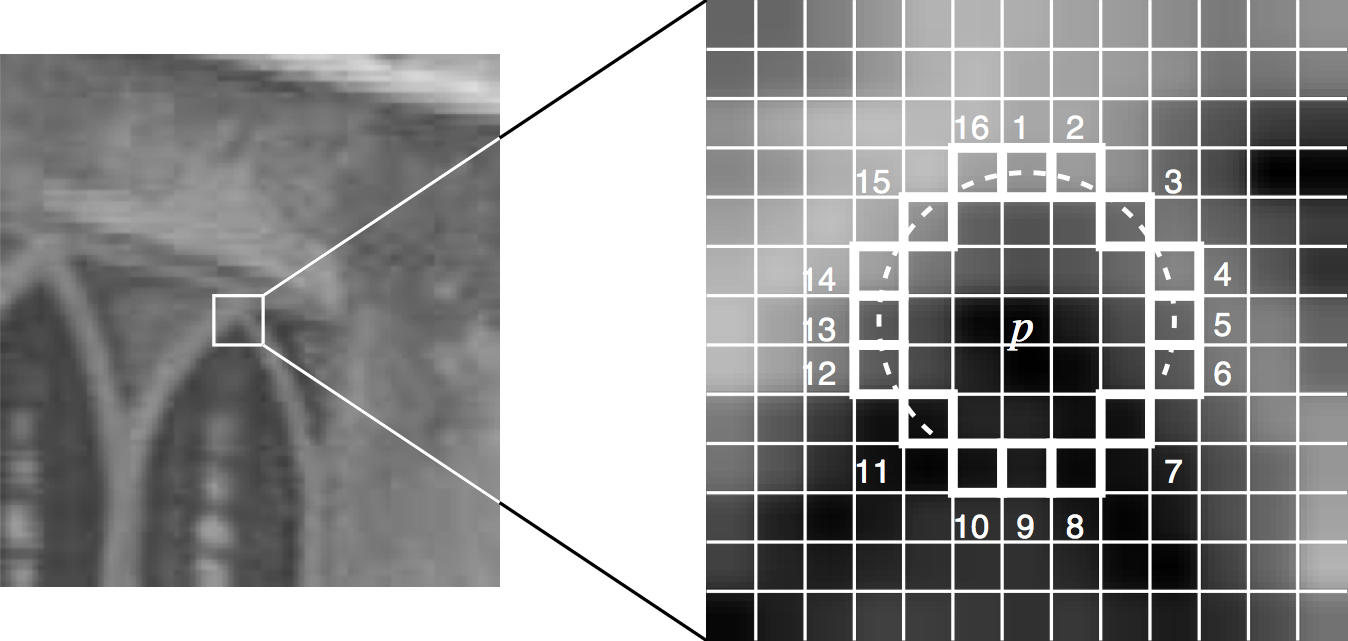
\includegraphics[width=380pt]{chapters/tracking_library_for_the_web/fast.png}
  \caption{Point segment test corner detection in an image patch \cite{Glass2013}.}
  \label{figure:fast}
\end{figure}

% subsection feature_detector (end)

\subsection{Feature Extractors} % (fold)
\label{sub:tracking_library_for_the_web:marker_less_tracking_algorithm:feature_extractors}

To estimate motion, one can then match sets of features \{$m_{i}$\} and \{$m'_{j}$\} extracted from two images taken from similar, and often successive, viewpoints. A classical procedure \cite{Calonder2010} runs as follows. For each point \{$m_{i}$\} in the first image, search in a region of the second image around location \{$m_{i}$\} for point \{$m'_{j}$\}. The search is based on the similarity of the local image windows, also knowns as kernel windows, centered on the points, which strongly characterizes the points when the images are sufficiently close \cite{Lepetit2005}.

\begin{figure}[!htb]
  \centering
  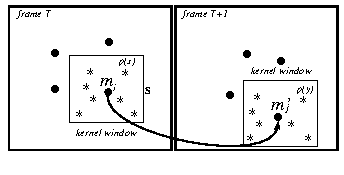
\includegraphics[width=\linewidth]{chapters/tracking_library_for_the_web/BRIEF.pdf}
  \caption{BRIEF \cite{Lepetit2005} feature extractor.}
  \label{figure:BRIEF}
\end{figure}

The feature matching used in the case studies performed in this work search for correspondent points in the current frame. Only points that are highly descriptive invariant features, called keypoints, are tested. Those keypoints were detected using FAST \cite{Rosten2010} in Section \ref{sub:tracking_library_for_the_web:marker_less_tracking_algorithm:feature_detector}. After the keypoints are detected they need to be described and the respective matching point should be found. Since web and handled devices have limited computational power having local descriptors that are fast to compute, to match and being memory efficient are important aspects, for that reason, was used an efficient method called Binary Robust Independent Elementary Features (BRIEF) \cite{Calonder2010}.

To generate the binary string for each key-point found in the smoothed frame, the individual bits are obtained by comparing the intensities of pairs of points, $(\textbf{p}; x, y)$, represented by $\ast$ symbol on Figure \ref{figure:BRIEF}, along the kernel window centered on each key-point without requiring a training phase.
Empirically, this technique shows that $256$ or even $128$ bits \cite{Calonder2010}, often suffice to obtain very good matching results. The best spatial arrangement of the tested (\textbf{x}, \textbf{y})-pairs of points are reach when selected based on an isotropic Gaussian distribution \cite{Calonder2010}. To compute the Gaussian distribution can be time consuming. As an optimization proposed by this article, the Gaussian distribution could be simply replaced by a random function due to its random characteristics.

To generate the binary strings is defined test $\tau$ on patch \textbf{p} of size \textbf{S $\times$ S} as

$$\tau(\textbf{p}; x, y) :=
\begin{cases}
  1 &\mbox{if}\quad \textbf{p(x)} < \textbf{p(y)},\\
  0 &\mbox{otherwise}
\end{cases}$$

where \textbf{p(x)} is the pixel intensity. The set of binary tests is defined by the $n_{d}$ (\textbf{x}, \textbf{y})-location pairs uniquely chosen during the initialization. The $n_{d}$-dimensional bit-string is our BRIEF descriptor for each key-point

$$f_{n_{d}}(\textbf{p}) := \sum_{1 \le i \le n_{d}} 2^{i-1} \tau(\textbf{p}; x, y).$$

In \cite{Calonder2010}, $n_{d}= 128, 256, 512$ were used in the tests and any of those values yield good compromises between speed, storage efficiency, and recognition rate. In this article, $n_{d}= 128$ was used, since it presented good matching results and performance. The number of bytes required to store the descriptor can be calculated by $k = n_{d}/8$, proving that BRIEF is also a memory-efficient method. Detailed results can be found in Chapter \ref{cha:evaluation}.

Once each keypoint is described with its binary string \cite{Calonder2010}, they need to be compared with the closest matching point. Distance metric is critical to the performance of intrusion detection systems. Thus using binary strings reduces the size of the descriptor and provides an interesting data structure that is fast to operate with whose similarity can be measured by the Hamming distance which, on desktop implementations, the computation time could be driven almost to zero using the POPCNT instruction from SSE4.2 \cite{Intel2007}. Only the latest Intel Core i7 CPUs support this instruction.

The Hamming distance is an important step on feature matching, it provides a fast and memory-efficient way to calculate distance between binary strings. Given two image patches $x$ and $y$, denote their binary descriptors as $b(x) \in \{0,1\}^n$ and $b(y) \in \{0,1\}^n$ respectively. Then their Hamming distance is computed by:

$$Ham(x, y)=\sum_{i=1}^{n}b_i(x)\otimes b_i(y)$$

In which $n$ is the dimension of binary descriptor and stands for bitwise XOR operation. According to the definition of Hamming distance, all the elements of a binary descriptor contribute equally to the distance. From the hamming distance, the Hamming weight can be calculated. It is used to find the best feature point match. Here, is generalized the Hamming distance to the weighted Hamming:

$$WHam(x, y)=\sum_{i=1}^{n}w_i(b_i(x)\otimes b_i(y))$$

Where $w_i$ is the weight of the $i$th element. The goal is to learn $w_i,i=1,2\cdots,n$ for the binary descriptor (BRIEF) based on a set of feature points. By assigning different weights to binary codes, what we expect is to obtain a distance space in which the distances of matching patches are less than those of non-matching patches.

% subsection feature_extractors (end)

\subsection{Homography Estimation} % (fold)
\label{sub:tracking_library_for_the_web:marker_less_tracking_algorithm:homography_estimation}

Typically, homographies are estimated between images by finding feature correspondences in those images. A 2D point $(x,y)$ in an image can be represented as a 3D vector $\textbf{x} = (x_1, x_2, x_3)$ where $x = \frac{x_1}{x_3}$ and $y = \frac{x_2}{x_3}$ \cite{Homography2009}. This is called the homogeneous representation of a point and it lies on the projective plane $P^2$. A homography is an invertible mapping of points and lines on the projective plane $P^2$. Hartley and Zisserman \cite{Hartley2004} provide the specific definition that a homography is a mapping from $P^2$ → $P^2$ is a projectivity if and only if there exists a non-singular $3\times3$ matrix $H$ such that for any point in $P^2$ represented by vector $\textbf{x}$ it is true that its mapped point equals $H\textbf{x}$. It should be noted that $H$ can be changed by multiplying by an arbitrary non-zero constant without altering the projective transformation. Thus $H$ is considered a homogeneous matrix and only has $8$ degrees of freedom even though it contains $9$ elements.

The method chosen to solve the homography estimation was the Direct Linear Transformation (DLT) \cite{Impa2009,Hartley2004} algorithm. The DLT algorithm is a simple algorithm used to solve for the homography matrix $H$ given a sufficient set of point correspondences \cite{Homography2009}.

Since we are working in homogeneous coordinates, the relationship between two corresponding points $\textbf{x}$ and $\textbf{x'}$ can be re-written as \cite{Homography2009}:

$$c\begin{pmatrix}u\\ v\\ 1\\\end{pmatrix} = H\begin{pmatrix}x\\ y\\ 1\\\end{pmatrix} \;\; \forall \;\; H=\begin{pmatrix}h1 & h2 & h3\\ h4 & h5 & h6\\ h7 & h8 & h9\\\end{pmatrix},$$

where $c$ is any non-zero constant, $(\; u \; v \; 1 \;)^T$ represents $\textbf{x'}$, $(\; x \; y \; 1 \;)^T$ represents $\textbf{x}$. Dividing the first row of equation (2.1) by the third row and the second row by the third row we get the following two equations \cite{Homography2009}:

\begin{equation}
\label{eq:homography1}
-h1x-h2y-h3 +(h7x+h8y+h9)u=0
\end{equation}
\begin{equation}
\label{eq:homography2}
-h4x-h5y-h6 +(h7x+h8y+h9)u=0
\end{equation}

Equations (\ref{eq:homography1}) and (\ref{eq:homography2}) can be written in matrix form as $A_i\textbf{h}=0$. Where,

$$A_i=\begin{pmatrix}-x & -y & -1 & 0 & 0 & 0 & ux & uy & u\\0 & 0 & 0 & -x & -y & -1 & vx & vy & v\end{pmatrix}$$

and

$$\textbf{h}=\begin{pmatrix}h1 & h2 & h3 & h4 & h5 & h6 & h7 & h8 & h9\end{pmatrix}.$$

Since each point correspondence provides $2$ equations, $4$ correspondences are sufficient to solve for the $8$ degrees of freedom of $H$. JavaScript typed arrays, defined in Section \ref{sub:basic_concepts:web:javascript_typed_arrays}, were used in the homography estimation implementation for better performance results.

% subsection homography_estimation (end)

\subsection{Random Sample Consensus (RANSAC)} % (fold)
\label{sub:tracking_library_for_the_web:marker_less_tracking_algorithm:ransac}

RANSAC (Random Sample Consensus) \cite{Hartley2004} is the most commonly used robust estimation method for homographies according to \cite{Homography2009}. The idea of the algorithm is pretty simple; For a number of iterations, a random sample of $4$ correspondences is selected and a homography $H$ is computed from those four correspondences. Each other correspondence is then classified as an inlier or outlier depending on its concurrence with $H$. After all of the iterations are done, the iteration that contained the largest number of inliers is selected. $H$ can then be recomputed from all of the correspondences that were consider as inliers in that iteration \cite{Homography2009}.

One important step when applying the RANSAC algorithm described above is to decide how to classify correspondences as inliers or outliers. In the implementation for the web only assign the geometric distance \cite{Homography2009} threshold, $t$, between $\textbf{x'}$ and $H\textbf{x}$ was enough. Hartley and Zisserman \cite{Hartley2004} provides more details about RANSAC.

Another issue is to decide how many iterations to run the algorithm, it's not required to try every combination of 4 correspondences. The goal becomes to determine the number of iterations, $N$, that ensures with a probability $p$ that at least one of the random samples will be free from outliers. $N=100$ was used on the web implementation.

% subsection ransac (end)

% section marker_less_tracking_algorithm (end)

\section{Rapid Object Detection (Viola Jones)} % (fold)
\label{sec:tracking_library_for_the_web:rapid_object_detection}

\subsection{Contextualization} % (fold)
\label{sub:tracking_library_for_the_web:rapid_object_detection:contextualization}

Rapid Object Detection \cite{Viola2001} technique, much known as Viola Jones \cite{Viola2001}, brings together new algorithms and insights to construct a library for robust and extremely rapid object detection. What has motivated this technique to be added to \textit{tracking.js} library was the task of face detection. Surprisingly, the algorithm became robust enough to detect any training data \cite{Viola2001}, not only for faces. Currently, \textit{tracking.js} supports, face, eyes, upper body and palm detection.

In order to scan faces, eyes or palm from images, a training phase is required. The training phase generate cascading stages. The cascade are constructed by training classifiers using AdaBoost \cite{Viola2001} and then adjusting the threshold to minimize false negatives. OpenCV library \cite{Bradski2000} has some open-source training data, therefore doubling efforts on training is unnecessary, \ie\ the face training set consisted of 4916 faces, extracted from images downloaded during a random crawl of the world wide web \cite{Viola2001}. Those faces were scaled and aligned to a base resolution of $24$ by $24$ pixels \cite{Viola2001}, see Figure \ref{figure:viola_training}. Training is not the focus of this work, the algorithm to scan the faces is. The training data itself is useless if a Scanning Detector \cite{Viola2001} is not available, the scanning is what makes the rapid object detection.

\begin{figure}[!htb]
  \centering
  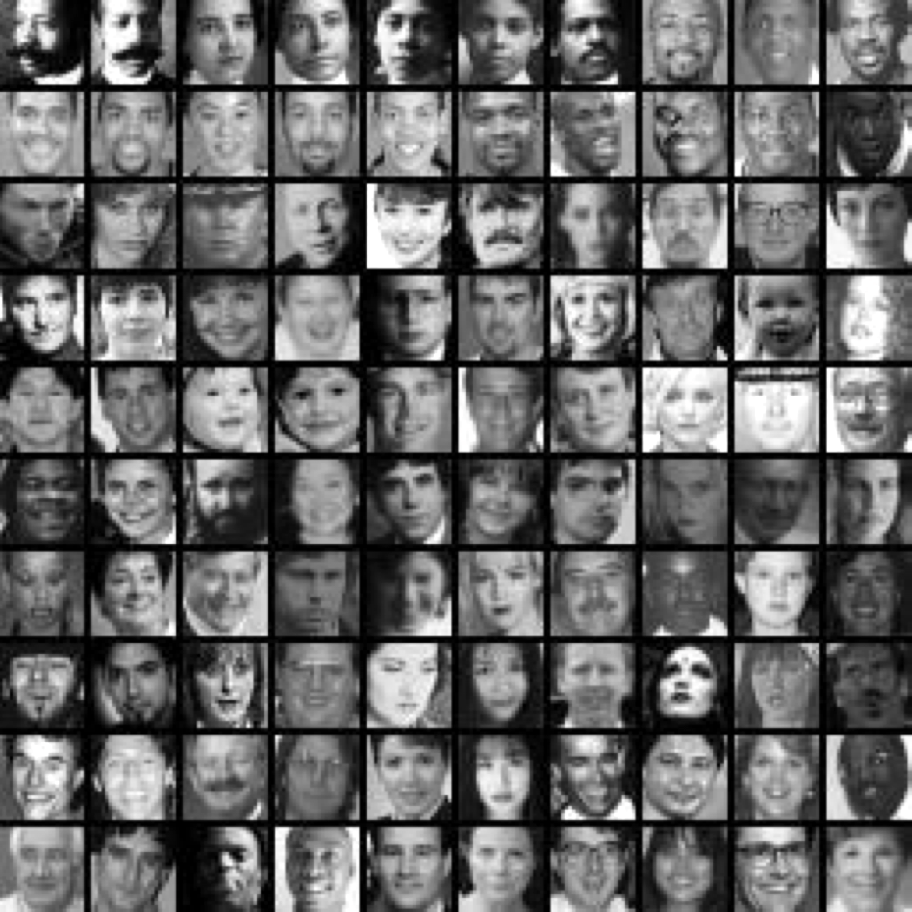
\includegraphics[width=240pt]{chapters/tracking_library_for_the_web/viola_training.png}
  \caption{Example of frontal upright face images used for training \cite{Viola2001}.}
  \label{figure:viola_training}
\end{figure}

A scanning detector was implemented in JavaScript \cite{International2009} and is available on \textit{tracking.js}. The training data used is from OpenCV library \cite{Bradski2000} converted from Extensible Markup Language (XML) \cite{Bray2013} to JavaScript Object Notation (JSON) \cite{Crockford2013}. JSON \cite{Crockford2013} has much superior performance since it's interpreted by JavaScript language \cite{International2009,Crockford2013}. The results of the JavaScript \cite{International2009} implementation can be used in real-time applications, the detector runs at 15 frames per second. For more information about performance see Chapter \ref{cha:evaluation}.

The overall idea of the detection process is that it uses a degenerate decision tree, what Viola and Jones \cite{Viola2001} call ``cascade''. A positive result from the first classifier triggers the evaluation of a second classifier which has also been adjusted to achieve very high detection rates \cite{Viola2001}. A positive result from the second classifier triggers a third classifier, and so on \cite{Viola2001}. The main steps of the scanning algorithm are:

\begin{enumerate}
  \item Create or scale a squared block, initially set to $20\times20$ pixels, by $1.25$ per iteration;
  \item Loop the squared block by $\Delta$ pixels over the image;
  \item For each squared block location, loop the decision tree and evaluate each stage;
  \item A positive result of the stage \cite{Viola2001} triggers the next stage, otherwise stops the stages loop;
  \item If all stages were positively evaluated store that rectangle as a possible face;
  \item Once the decision tree is done, group the overlapping rectangles;
  \item Find the best rectangle of each the group to represent the face. This phase is also known as ``merging phase''.
\end{enumerate}

The final detector is scanned across the image at multiple scales and locations of the image. This process makes sense because the features can be evaluated at any scale with the same cost \cite{Viola2001}. Good results were obtained using a set of scales a factor of $1.25$. Subsequent locations are obtained by shifting the window some number of pixels $\Delta$, for a better accuracy $\Delta=1$ is recommended. We can achieve a significant speedup by setting $\Delta=2$ with only a slight decrease in accuracy, thus this value was set as default value of the JavaScript \cite{International2009} implementation.

Viola and Jones \cite{Viola2001} proposed that for each found possible rectangle representing the face to be partitioned into disjoint subsets data structures. Two detections are in the same subset if their bounding regions overlap \cite{Viola2001}. The corners of the final bounding region are the average of the corners of all detections in the set. In order to perform well on the web, some optimizations were made in the implementation level of the scanning detector. The disjoint set was replaced by an alternative logic that is called ``Minimum Neighbor Area Grouping'' by this thesis. Minimum Neighbor Area Grouping has $O(N^2)$ performance \cite{black2007big} and consists in a loop trough the possible rectangle faces returned by the scanning detector. For each step of the loop compare the current rectangle with all other not yet compared rectangles. If the rectangle area overlaps more than $\eta$ with the compared, by default $\eta=0.5$ (or $50\%$), select the smallest rectangle in area of the comparison. Using the smallest rectangle, guarantees that the best match is much centralized in the face.

For more information about the JavaScript \cite{International2009} implementation, such as evaluation and results, see Chapter \ref{cha:evaluation}.

% subsection contextualization (end)

% section rapid_object_detection (end)

\section{Color Tracking Algorithm} % (fold)
\label{sec:tracking_library_for_the_web:color_tracking_algorithm}

\subsection{Contextualization} % (fold)
\label{sub:tracking_library_for_the_web:color_tracking_algorithm:contextualization}

Colors are part of our lives, they are everywhere in every single object. Being able to use colored objects to control your browser using the user camera is very appealing. For that reason, \textit{training.js} implemented a basic color tracking algorithm that resulted in an real-time frame rate trough a simple and intuitive API.

% subsection contextualization (end)

% section color_tracking_algorithm (end)

% chapter tracking_library_for_the_web (end)
\chapter{Tracking Library for the Web (tracking.js)} % (fold)
\label{cha:tracking_library_for_the_web}

\section{Contextualization} % (fold)
\label{sec:tracking_library_for_the_web:Contextualization}

The desktop platform is the target environment most commonly addressed when developing AR systems. However, depending on the requirements of an AR application, the use of different execution platforms may be necessary. If the system has to be published to several users, the web platform shows to be more adequate, where the application is executed through the Internet in a web browser \cite{Pablo2013}.
The use of markerless tracking, which is based on natural features of the scene, has also been gaining more space on web targeted AR applications for advertising. The media used in this kind of application needs to be as appealing as possible in order to catch consumers' attention. Markerless tracking satisfies this requirement, since the idea of having a real scene augmented with virtual objects without any artificial elements such as markers added to the environment is very attractive \cite{Pablo2013}. In addition, the product being advertised can be tracked and augmented with virtual elements \cite{Pablo2013}.
Browsers are evolving very fast when compared to the the previous decade \cite{Hickson2013}. JavaScript language \cite{International2009,MDN2013} wasn't prepared to handle typed data structures \cite{TypedArray2013} able to manipulate raw binary data safely \cite{Canvas2013}, all the computational complexity required by AR algorithms was too much for that growing environment. Browsers weren't able to capture audio and video \cite{MediaCapture2013,WebRTC2013} natively, without plugin installation \cite{Flash2013}, an essential feature for AR applications. This reality has changed, this involves the use of several modern browser specifications \cite{Hickson2013,WC2006} as well as implementation of different computer vision algorithms and techniques into the browser environment taking advantage of all those modern APIs \cite{Hickson2013,WC2006}.

In this context, this thesis aims to present the implementation and evaluation of a solution regarding tracking techniques for web targeted AR. The available algorithms and techniques can be used for different applications, such as, detect faces, identify objects and colors and track moving objects. The solution is called \textit{tracking.js}. Some optimizations are discussed and implemented on this work in order to achieve good results when compared with similar implementations in compiled languages.

\subsection{Related Work} % (fold)
\label{sub:tracking_library_for_the_web:related_work}

There are not many web based RA solutions available and registered in the literature. The ones available are mainly focused on fiducial markers \cite{Cho1998}, such as FLARToolKit \cite{Yan2011} and JSARToolkit \cite{JSARToolkit2011}, they both are ports of ARToolKit \cite{Hirokazu2002}. ARToolKit is a desktop library which is useful to make vision-based AR applications \cite{Hirokazu2002}. The Metaio company developed Unifeye Viewer \cite{Metaio2009}, a proprietary plug-in for Flash \cite{Flash2013} that allows the utilization of markerless AR applications on the web. In order to run Flash \cite{Flash2013} based applications, the installation of its plugin is required. Third-party plugins, such as Flash \cite{Flash2013}, are in decadency on modern and mobile web browsers, instead JavaScript \cite{International2009} based solutions are preferred, since they can run in any modern browser without requiring any user effort of installing external software. Some smart-phones don't even support Flash \cite{Flash2013} plugin into their browsers, \eg\ Safari for mobile \cite{Safari2013} is one example of a mobile browser that has banned Flash \cite{Flash2013}.

\begin{enumerate}
    \item FLARToolKit: is a port of the well-known ARToolKit \cite{Hirokazu2002} marker tracking library to ActionScript \cite{Flash2013}, which is the language utilized in the development of Flash \cite{Flash2013} applications for the web. This was the first initiative towards AR solutions for the web \cite{Pablo2013}. Using FLARToolKit \cite{Yan2011}, is possible to develop AR applications that runs on client's browser. A marker based AR example for the web, developed for a marketing campaign of General Electric's company using FLARToolKit, is shown on Figure \ref{figure:flartoolkit}.

    \begin{figure}[!htb]
      \centering
      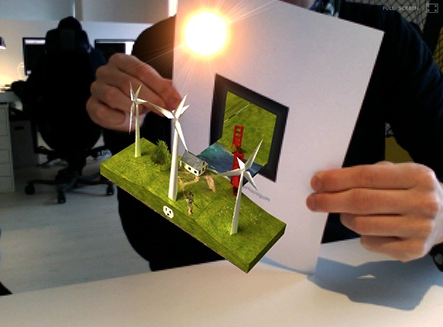
\includegraphics[width=240pt]{chapters/tracking_library_for_the_web/flartoolkit.png}
      \caption{Marker based AR for the web using FLARToolKit.}
      \label{figure:flartoolkit}
    \end{figure}

    \item JSARToolkit: is a JavaScript \cite{International2009} port of FLARToolKit \cite{Yan2011}, operating on canvas images \cite{Canvas2013} and
video element \cite{Hickson2013} contents, provides another marker tracking library. This was the first, open-source, JavaScript \cite{International2009} based, AR solution available for the web. A marker based AR example for the web using JSARToolKit is shown on Figure \ref{figure:jsartoolkit}.

    \begin{figure}[!htb]
      \centering
      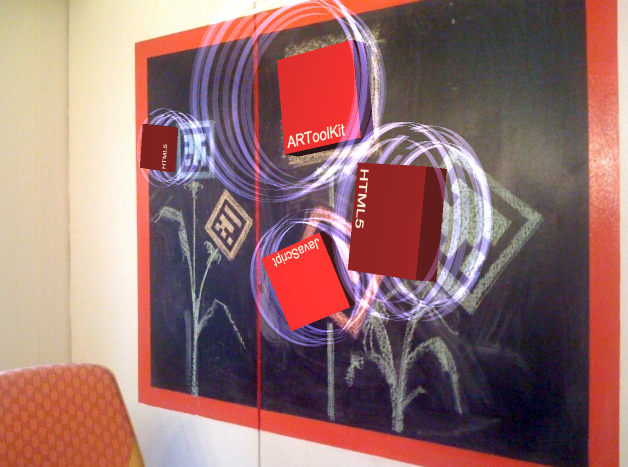
\includegraphics[width=240pt]{chapters/tracking_library_for_the_web/jsartoolkit.png}
      \caption{Marker based AR for the web using JSARToolKit.}
      \label{figure:jsartoolkit}
    \end{figure}

    \item Unifeye Viewer: from Metaio company, offers a robust markerless tracking solution for the web. Unifeye \cite{Metaio2009} also depends on Flash \cite{Flash2013} plugin in order to run on web browsers. A similar example of General Electric's marker based solution, this time markerless based, is shown on Figure \ref{figure:unifeyeviewer}. Note that the 3D image is projected over a magazine cover instead of a fiducial marker \cite{Cho1998}.

    \begin{figure}[!htb]
      \centering
      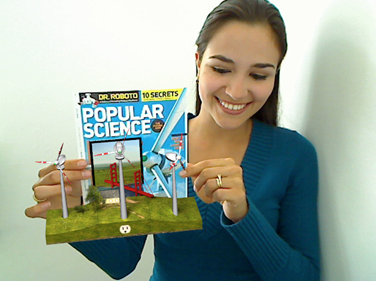
\includegraphics[width=240pt]{chapters/tracking_library_for_the_web/unifeyeviewer.png}
      \caption{Markerless example of image projected over a magazine cover using Unifeye Viewer solution.}
      \label{figure:unifeyeviewer}
    \end{figure}
\end{enumerate}

There is a disadvantage of using marker based AR. Depend on a artificial marker in order to augment the scene with virtual elements is counterintuitive. Commonly, web applications are utilized by novice users that do not have sufficient technical knowledge to perform manual setup, such as print fiducial markers or perform manual initialization for the tracking. FLARToolKit \cite{Yan2011} and JSARToolkit \cite{JSARToolkit2011} are both marker based techniques, using Flash \cite{Flash2013} and JavaScript \cite{International2009}, respectively. FLARToolKit has one more issue which is dependency on Flash \cite{Flash2013} plugin installation. Unifeye Viewer by Metaio, was the only existing solution that provided markerless tracking for the web, although it uses Flash \cite{Flash2013}, excluding it from a potential competitor of \textit{tracking.js}. Markerless tracking techniques do not depend on any artificial marker or advanced user initialization. The space on web targeted AR applications for advertising is gaining more space and the media used in this kind of application needs to be as appealing as possible \cite{Pablo2013}. Making markerless tracking a suitable technique to such applications.

The solution proposed in this thesis, \textit{tracking.js}, provides the first known, open-source, markerless tracking solution for the web that runs entirely in JavaScript \cite{International2009} and HTML5 \cite{Hickson2013}.

% subsection related_work (end)

\subsection{Library Modules} % (fold)
\label{sub:tracking_library_for_the_web:library_modules}

The proposed library is divided in modules in order to allow extension and addition of new features, such as new RA techniques or math utilities. For a better understanding of the library architecture, the current implementation is divided in two packages separating Base from AR classes. Base classes modules are shown in Figure \ref{figure:base_classes} and AR classes in Figure \ref{figure:ar_classes}.

To develop AR applications using only raw JavaScript \cite{International2009} APIs \cite{MDN2013} could be too verbose and complex, \eg\ capturing users' camera and reading its array of pixels. The big amount of steps required for a simple task makes web developers life hard when the goal is to achieve complex implementations. Some level of encapsulation is needed in order to simplify development. The proposed library provides encapsulation for common tasks on the web platform.

The two main available packages splits Base from AR classes. Furthermore, each class of those packages are described. Let's start with the base classes:

\begin{enumerate}
  \item Math: provides common math utilities optimized for the web, such as geometry, linear algebra \cite{Hartley2004} and hamming operations. Typed arrays \cite{TypedArray2013} are used in order to optimize performance, see subsection \ref{sub:basic_concepts:web:javascript_typed_arrays} for more information about typed arrays.
  \item Attribute: allows developers to add attributes to any class through an Attribute interface. The interface adds get and set methods to your class to retrieve and store attribute values, as well as support for change events that can be used to listen for changes in attribute values.
  \item DOMElement: provides a way to create, and manipulate HTML \cite{Hickson2013} DOM nodes \cite{WC2006}. Each DOMElement instance represents an underlying DOM node \cite{WC2006}. In addition to wrapping the basic DOM API \cite{WC2006} and handling cross browser issues, Nodes provide convenient methods for managing styles and subscribing to events.
  \item Canvas: provides an utility class to create, and manipulate HTML5 \cite{Hickson2013} canvas element \cite{Canvas2013}. Each Canvas instance represents an underlying canvas DOM node \cite{Canvas2013}. In addition to wrapping the basic DOM API \cite{WC2006}, also provides methods to extract via \textit{getImageData} method, to loop via \textit{forEach} method, and to set the canvas array of pixels via \textit{setImageData} method.
  \item Video: provides an utility class to create, and manipulate HTML5 \cite{Hickson2013} video element. Each Video instance represents an underlying video DOM node \cite{Canvas2013}. In addition to wrapping the basic DOM API \cite{WC2006}, also provides methods to \textit{play}, \textit{pause} and register tracker algorithms via \textit{track} method. See subsection \ref{sub:basic_concepts:web:audio_and_video} for more information about video element.
  \item VideoCamera: extends all functionalities from Video class with the addition of capturing the user camera via \textit{capture} method. The underlying implementation uses WebRTC \cite{WebRTC2013} and Media Capture and Streams \cite{MediaCapture2013} specifications.
\end{enumerate}

Visual tracking classes includes several computer vision algorithms, such as FAST \cite{RostenFaster2010}, BRIEF \cite{Calonder2010} implementations, homography estimation and others. As the library grows, many other computer vision algorithms are going to be added to the library, such as 3D pose calculation.

\begin{enumerate}
  \item FAST: provides an implementation of Features from Accelerated Segment Test (FAST) \cite{Rosten2010} for features detection via \textit{findCorners(data, threshold)} method, where $data$ is the \textit{ImageData} of the canvas \cite{Canvas2013} frame. It also depends on a $threshold$ argument. The pixel at $p$, see Figure \ref{figure:fast}, is the center of a candidate corner and they are classified if brighter than $p$ by more than the $threshold$.
  \item BRIEF: provides an implementation of Binary Robust Independent Elementary Features (BRIEF) \cite{Calonder2010} for feature extraction via \textit{getDescriptors(data, corners)} method and matching via \textit{match(c1, d1, c2, d2)}, where $data$ is an \textit{ImageData}, and $c1$ and $c2$ are the found corners array return by \textit{FAST.findCorners} method and $d1$ and $d2$ are feature descriptors array return by \textit{BRIEF.getDescriptors} method.
  \item RANSAC: provides an interface used to achieve robust estimation method for homographies and camera pose. There are two available estimation methods implemented that inherits from RANSAC \cite{Hartley2004}, Homography and Pose.
  \item Homography: provides an API to estimate a homography matrix $H$ between images by finding feature correspondences in those images.
  \item Pose: TODO.
  \item ViolaJones: TODO.
  \item Color: TODO.
\end{enumerate}

\begin{figure}[!htb]
    % \tikzumlset{font=\scriptsize}
    \begin{tikzpicture}
        \begin{umlpackage}{Base classes}

            \umlclass[y=-50pt,x=190pt]{Math}{}{
              createIdentityMatrix(size) : Matrix\\
              distance(x1, y1, x2, y2) : Number\\
              getDeterminant(Matrix) : Number\\
              getInverse(Matrix) : Matrix\\
              hammingDistance(n1, n2) : Number\\
              hammingWeight(number) : Number\\
              ...
            }

            \umlclass{Attribute}{}{
              get(name) : Object\\
              set(name, value) : void \\
            }

            \umlclass[y=-100pt]{DOMElement}{
              width : Number\\
              height : Number\\
              visible : boolean\\
            }{
              show() : void\\
              hide() : void \\
            }

            \umlclass[y=-220pt,x=180pt]{Canvas}{
              context : Object
            }{
              forEach(data, callback) : void\\
              getImageData(x, y, width, height) : ImageData \\
              setImageData(data, x, y) : void\\
            }

            \umlclass[y=-335pt]{Video}{}{
              play() : void\\
              pause() : void\\
              track(tracker) : void \\
              getVideoCanvasImageData(x, y, width, height) : ImageData \\
            }

            \umlclass[y=-335pt,x=220pt]{VideoCamera}{}{
              capture() : void \\
            }

        \end{umlpackage}

        \umlinherit[geometry=-|]{DOMElement}{Attribute}
        \umlinherit[geometry=-|]{Canvas}{DOMElement}
        \umlinherit[geometry=-|]{Video}{DOMElement}
        \umlinherit[geometry=|-]{VideoCamera}{Video}
    \end{tikzpicture}
    \caption{Base classes of tracking.js library.}
    \label{figure:base_classes}
\end{figure}

\begin{figure}[!htb]
    % \tikzumlset{font=\scriptsize}
    \begin{tikzpicture}
        \begin{umlpackage}{Visual tracking classes}

            \umlclass{FAST}{}{
              findCorners(data, threshold) : Array\\
            }

            \umlclass[y=-70pt]{BRIEF}{}{
              getDescriptors(data, corners) : Array\\
              match(c1, d1, c2, d2) : Array\\
            }

            \umlclass[y=-150pt]{ViolaJones}{}{
              find() : Array\\
              evalStage() : boolean\\
            }

            \umlclass[y=-225pt]{Color}{}{
              find() : Array\\
            }

            \umlclass[x=200pt]{RANSAC}{}{
              find(matches) : void\\
              score() : Number\\
            }

            \umlclass[y=-90pt,x=200pt]{Homography}{}{
                score(H, matches) : Number\\
            }

            \umlclass[y=-170pt,x=200pt]{Pose}{}{
              find(points2d, points3d) : void\\
            }

        \end{umlpackage}

        \umlinherit[geometry=-|]{Homography}{RANSAC}
        \umlinherit[geometry=-|]{Pose}{RANSAC}
    \end{tikzpicture}
    \caption{Visual tracking classes of tracking.js library.}
    \label{figure:ar_classes}
\end{figure}

\newpage

% subsection library_modules (end)

% section contextualization (end)

\section{Markerless Tracking Algorithm} % (fold)
\label{sec:tracking_library_for_the_web:marker_less_tracking_algorithm}

\subsection{Contextualization} % (fold)
\label{sub:tracking_library_for_the_web:marker_less_tracking_algorithm:contextualization}

Lorem ipsum dolor sit amet, consectetur adipisicing elit.

% subsection contextualization (end)

\subsection{Feature Detector} % (fold)
\label{sub:tracking_library_for_the_web:marker_less_tracking_algorithm:feature_detector}

This technique relies on matching individual features across images and are therefore easy to increase robustness against partial occlusions or matching errors. Illumination invariance is also simple to achieve. Feature points detection is used as the first step of many vision tasks such as tracking, localization, image matching and recognition. In this article we call ``feature'' or ``keypoint'' to refer to a point of interest in two dimensions.

For each frame, the object features are matched by localizing feature templates in search windows around hypothesized locations \cite{Lepetit2005}. The method to extract feature points suggested in Features from Accelerated Segment Test (FAST) \cite{Rosten2010}. FAST \cite{RostenFaster2010} hypothesizes the matches using corner detection. A large number of corner detectors exist in the literature. However, we have a strong interest in real time frame rate applications which computational resources are required requisites. The approach proposed by FAST \cite{RostenFaster2010} allows the detector to produce a suite of high-speed detectors which we currently use for real-time tracking and AR label placement \cite{Calonder2010}. In particular, it is still true that when processing live video streams at full frame rate, existing feature detectors leave little if any time for further processing, even despite the consequences of Moore's Law \cite{Rosten2010}.

To show that speed can been obtained without necessarily sacrificing the quality of the feature detector, in Chapter \ref{cha:evaluation}, we compare our detector, to a variety of well-known detectors. A number of the detectors described below compute a corner response, (1) Edge based corner detectors, corresponds to the boundary between two regions; (2) Gray level derivative based detectors, the assumption that corners exist along edges is an inadequate model for patches of texture and point like features, and is difficult to use at junctions. Therefore a large number of detectors operate directly on gray level images without requiring edge detection; and (3) Direct gray level detectors, Another major class of corner detectors work by examining a small patch of an image to see if it ``looks'' like a corner \cite{Rosten2010}.

The thesis choice was (3) Direct gray level detectors. It works by testing a small patch of an image to see if it could be a corner. The detector is evaluated using a circle surrounding the candidate pixel, the test is based on whether the concentric contiguous arcs around the pixel are significantly different from the central pixel $p$ \cite{Rosten2010}. To classify $p$ as a corner should exists a set of $n$ contiguous pixels in the circle which are all brighter than the intensity of the candidate pixel $I_{p} + t$ (threshold), or all darker than $I_{p} - t$ \cite{Rosten2010}.

The number of contiguous tested pixels could vary accordingly \cite{Rosten2010}, being more common to be FAST-$12$ or FAST-$9$. Empirically, FAST-$9$ showed to have a good repeatability and a better efficiency on the web. The repeatability of found feature points is also important because determines whether the technique is useful in a real-world application.

This detector in itself exhibits high performance, but there are several weaknesses: (1) This high-speed test does not reject as many candidates; (2) The efficiency of the detector will depend on the ordering of the questions and the distribution of corner appearances; and (3) Multiple features are detected adjacent to one another \cite{Rosten2010}.

On Figure \ref{figure:fast}, the highlighted squares are the pixels used in the corner detection. The pixel at $p$ is the central pixel. The arc is indicating that the dashed line passes through FAST-$n$, let $n$ be $9$ or $12$ contiguous pixels which are brighter or darker than $p$ \cite{Rosten2010}.

\begin{figure}[!htb]
  \centering
  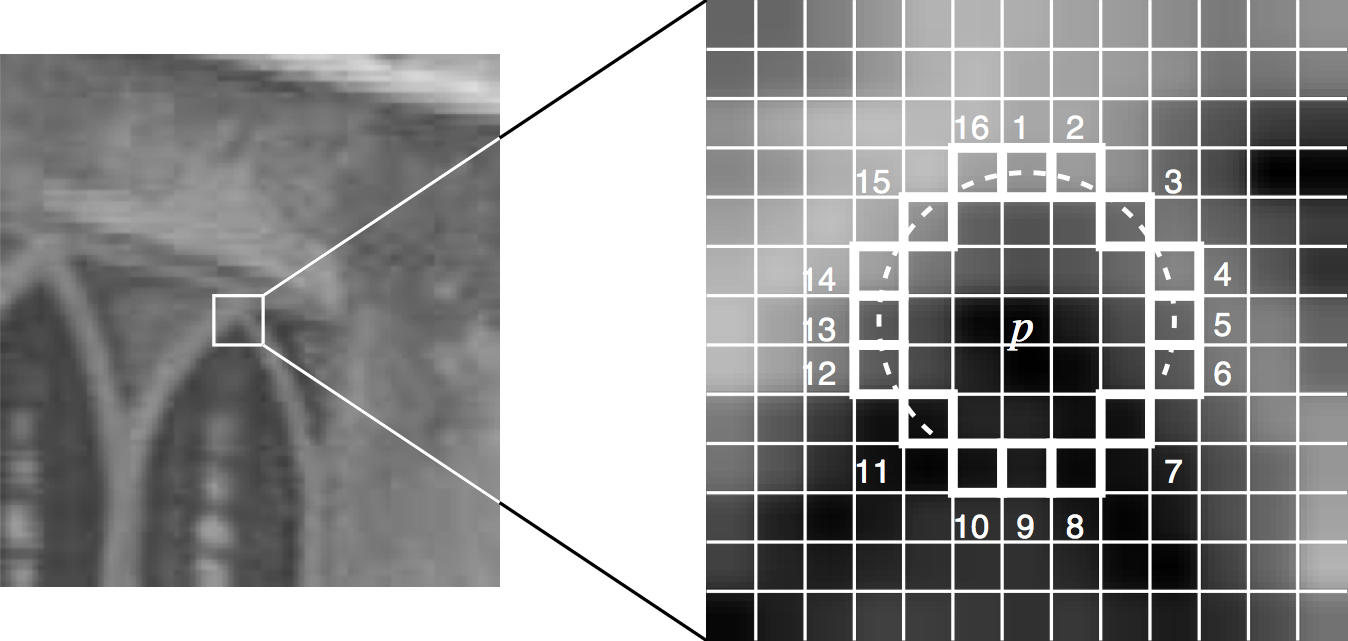
\includegraphics[width=380pt]{chapters/tracking_library_for_the_web/fast.png}
  \caption{Point segment test corner detection in an image patch \cite{Glass2013}.}
  \label{figure:fast}
\end{figure}

% subsection feature_detector (end)

\subsection{Feature Extractors} % (fold)
\label{sub:tracking_library_for_the_web:marker_less_tracking_algorithm:feature_extractors}

To estimate motion, one can then match sets of features \{$m_{i}$\} and \{$m'_{j}$\} extracted from two images taken from similar, and often successive, viewpoints. A classical procedure \cite{Calonder2010} runs as follows. For each point \{$m_{i}$\} in the first image, search in a region of the second image around location \{$m_{i}$\} for point \{$m'_{j}$\}. The search is based on the similarity of the local image windows, also knowns as kernel windows, centered on the points, which strongly characterizes the points when the images are sufficiently close \cite{Lepetit2005}.

\begin{figure}[!htb]
  \centering
  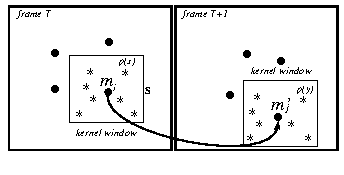
\includegraphics[width=\linewidth]{chapters/tracking_library_for_the_web/BRIEF.pdf}
  \caption{BRIEF \cite{Lepetit2005} feature extractor.}
  \label{figure:BRIEF}
\end{figure}

The feature matching used in the case studies performed in this work search for correspondent points in the current frame. Only points that are highly descriptive invariant features, called keypoints, are tested. Those keypoints were detected using FAST \cite{Rosten2010} in Section \ref{sub:tracking_library_for_the_web:marker_less_tracking_algorithm:feature_detector}. After the keypoints are detected they need to be described and the respective matching point should be found. Since web and handled devices have limited computational power having local descriptors that are fast to compute, to match and being memory efficient are important aspects, for that reason, was used an efficient method called Binary Robust Independent Elementary Features (BRIEF) \cite{Calonder2010}.

To generate the binary string for each key-point found in the smoothed frame, the individual bits are obtained by comparing the intensities of pairs of points, $(\textbf{p}; x, y)$, represented by $\ast$ symbol on Figure \ref{figure:BRIEF}, along the kernel window centered on each key-point without requiring a training phase.
Empirically, this technique shows that $256$ or even $128$ bits \cite{Calonder2010}, often suffice to obtain very good matching results. The best spatial arrangement of the tested (\textbf{x}, \textbf{y})-pairs of points are reach when selected based on an isotropic Gaussian distribution \cite{Calonder2010}. To compute the Gaussian distribution can be time consuming. As an optimization proposed by this article, the Gaussian distribution could be simply replaced by a random function due to its random characteristics.

To generate the binary strings is defined test $\tau$ on patch \textbf{p} of size \textbf{S $\times$ S} as

$$\tau(\textbf{p}; x, y) :=
\begin{cases}
  1 &\mbox{if}\quad \textbf{p(x)} < \textbf{p(y)},\\
  0 &\mbox{otherwise}
\end{cases}$$

where \textbf{p(x)} is the pixel intensity. The set of binary tests is defined by the $n_{d}$ (\textbf{x}, \textbf{y})-location pairs uniquely chosen during the initialization. The $n_{d}$-dimensional bit-string is our BRIEF descriptor for each key-point

$$f_{n_{d}}(\textbf{p}) := \sum_{1 \le i \le n_{d}} 2^{i-1} \tau(\textbf{p}; x, y).$$

In \cite{Calonder2010}, $n_{d}= 128, 256, 512$ were used in the tests and any of those values yield good compromises between speed, storage efficiency, and recognition rate. In this article, $n_{d}= 128$ was used, since it presented good matching results and performance. The number of bytes required to store the descriptor can be calculated by $k = n_{d}/8$, proving that BRIEF is also a memory-efficient method. Detailed results can be found in Chapter \ref{cha:evaluation}.

Once each keypoint is described with its binary string \cite{Calonder2010}, they need to be compared with the closest matching point. Distance metric is critical to the performance of intrusion detection systems. Thus using binary strings reduces the size of the descriptor and provides an interesting data structure that is fast to operate with whose similarity can be measured by the Hamming distance which, on desktop implementations, the computation time could be driven almost to zero using the POPCNT instruction from SSE4.2 \cite{Intel2007}. Only the latest Intel Core i7 CPUs support this instruction.

The Hamming distance is an important step on feature matching, it provides a fast and memory-efficient way to calculate distance between binary strings. Given two image patches $x$ and $y$, denote their binary descriptors as $b(x) \in \{0,1\}^n$ and $b(y) \in \{0,1\}^n$ respectively. Then their Hamming distance is computed by:

$$Ham(x, y)=\sum_{i=1}^{n}b_i(x)\otimes b_i(y)$$

In which $n$ is the dimension of binary descriptor and stands for bitwise XOR operation. According to the definition of Hamming distance, all the elements of a binary descriptor contribute equally to the distance. From the hamming distance, the Hamming weight can be calculated. It is used to find the best feature point match. Here, is generalized the Hamming distance to the weighted Hamming:

$$WHam(x, y)=\sum_{i=1}^{n}w_i(b_i(x)\otimes b_i(y))$$

Where $w_i$ is the weight of the $i$th element. The goal is to learn $w_i,i=1,2\cdots,n$ for the binary descriptor (BRIEF) based on a set of feature points. By assigning different weights to binary codes, what we expect is to obtain a distance space in which the distances of matching patches are less than those of non-matching patches.

% subsection feature_extractors (end)

\subsection{Homography Estimation} % (fold)
\label{sub:tracking_library_for_the_web:marker_less_tracking_algorithm:homography_estimation}

Typically, homographies are estimated between images by finding feature correspondences in those images. A 2D point $(x,y)$ in an image can be represented as a 3D vector $\textbf{x} = (x_1, x_2, x_3)$ where $x = \frac{x_1}{x_3}$ and $y = \frac{x_2}{x_3}$ \cite{Homography2009}. This is called the homogeneous representation of a point and it lies on the projective plane $P^2$. A homography is an invertible mapping of points and lines on the projective plane $P^2$. Hartley and Zisserman \cite{Hartley2004} provide the specific definition that a homography is a mapping from $P^2$ → $P^2$ is a projectivity if and only if there exists a non-singular $3\times3$ matrix $H$ such that for any point in $P^2$ represented by vector $\textbf{x}$ it is true that its mapped point equals $H\textbf{x}$. It should be noted that $H$ can be changed by multiplying by an arbitrary non-zero constant without altering the projective transformation. Thus $H$ is considered a homogeneous matrix and only has $8$ degrees of freedom even though it contains $9$ elements.

The method chosen to solve the homography estimation was the Direct Linear Transformation (DLT) \cite{Impa2009,Hartley2004} algorithm. The DLT algorithm is a simple algorithm used to solve for the homography matrix $H$ given a sufficient set of point correspondences \cite{Homography2009}.

Since we are working in homogeneous coordinates, the relationship between two corresponding points $\textbf{x}$ and $\textbf{x'}$ can be re-written as \cite{Homography2009}:

$$c\begin{pmatrix}u\\ v\\ 1\\\end{pmatrix} = H\begin{pmatrix}x\\ y\\ 1\\\end{pmatrix} \;\; \forall \;\; H=\begin{pmatrix}h1 & h2 & h3\\ h4 & h5 & h6\\ h7 & h8 & h9\\\end{pmatrix},$$

where $c$ is any non-zero constant, $(\; u \; v \; 1 \;)^T$ represents $\textbf{x'}$, $(\; x \; y \; 1 \;)^T$ represents $\textbf{x}$. Dividing the first row of equation (2.1) by the third row and the second row by the third row we get the following two equations \cite{Homography2009}:

\begin{equation}
\label{eq:homography1}
-h1x-h2y-h3 +(h7x+h8y+h9)u=0
\end{equation}
\begin{equation}
\label{eq:homography2}
-h4x-h5y-h6 +(h7x+h8y+h9)u=0
\end{equation}

Equations (\ref{eq:homography1}) and (\ref{eq:homography2}) can be written in matrix form as $A_i\textbf{h}=0$. Where,

$$A_i=\begin{pmatrix}-x & -y & -1 & 0 & 0 & 0 & ux & uy & u\\0 & 0 & 0 & -x & -y & -1 & vx & vy & v\end{pmatrix}$$

and

$$\textbf{h}=\begin{pmatrix}h1 & h2 & h3 & h4 & h5 & h6 & h7 & h8 & h9\end{pmatrix}.$$

Since each point correspondence provides $2$ equations, $4$ correspondences are sufficient to solve for the $8$ degrees of freedom of $H$. JavaScript typed arrays, defined in Section \ref{sub:basic_concepts:web:javascript_typed_arrays}, were used in the homography estimation implementation for better performance results.

% subsection homography_estimation (end)

\subsection{Random Sample Consensus (RANSAC)} % (fold)
\label{sub:tracking_library_for_the_web:marker_less_tracking_algorithm:ransac}

RANSAC (Random Sample Consensus) \cite{Hartley2004} is the most commonly used robust estimation method for homographies according to \cite{Homography2009}. The idea of the algorithm is pretty simple; For a number of iterations, a random sample of $4$ correspondences is selected and a homography $H$ is computed from those four correspondences. Each other correspondence is then classified as an inlier or outlier depending on its concurrence with $H$. After all of the iterations are done, the iteration that contained the largest number of inliers is selected. $H$ can then be recomputed from all of the correspondences that were consider as inliers in that iteration \cite{Homography2009}.

One important step when applying the RANSAC algorithm described above is to decide how to classify correspondences as inliers or outliers. In the implementation for the web only assign the geometric distance \cite{Homography2009} threshold, $t$, between $\textbf{x'}$ and $H\textbf{x}$ was enough. Hartley and Zisserman \cite{Hartley2004} provides more details about RANSAC.

Another issue is to decide how many iterations to run the algorithm, it's not required to try every combination of 4 correspondences. The goal becomes to determine the number of iterations, $N$, that ensures with a probability $p$ that at least one of the random samples will be free from outliers. $N=100$ was used on the web implementation.

% subsection ransac (end)

% section marker_less_tracking_algorithm (end)

\section{Rapid Object Detection (Viola Jones)} % (fold)
\label{sec:tracking_library_for_the_web:rapid_object_detection}

\subsection{Contextualization} % (fold)
\label{sub:tracking_library_for_the_web:rapid_object_detection:contextualization}

Rapid Object Detection \cite{Viola2001} technique, much known as Viola Jones \cite{Viola2001}, brings together new algorithms and insights to construct a library for robust and extremely rapid object detection. What has motivated this technique to be added to \textit{tracking.js} library was the task of face detection. Surprisingly, the algorithm became robust enough to detect any training data \cite{Viola2001}, not only for faces. Currently, \textit{tracking.js} supports, face, eyes, upper body and palm detection.

In order to scan faces, eyes or palm from images, a training phase is required. The training phase generate cascading stages. The cascade are constructed by training classifiers using AdaBoost \cite{Viola2001} and then adjusting the threshold to minimize false negatives. OpenCV library \cite{Bradski2000} has some open-source training data, therefore doubling efforts on training is unnecessary, \ie\ the face training set consisted of 4916 faces, extracted from images downloaded during a random crawl of the world wide web \cite{Viola2001}. Those faces were scaled and aligned to a base resolution of $24$ by $24$ pixels \cite{Viola2001}, see Figure \ref{figure:viola_training}. Training is not the focus of this work, the algorithm to scan the faces is. The training data itself is useless if a Scanning Detector \cite{Viola2001} is not available, the scanning is what makes the rapid object detection.

\begin{figure}[!htb]
  \centering
  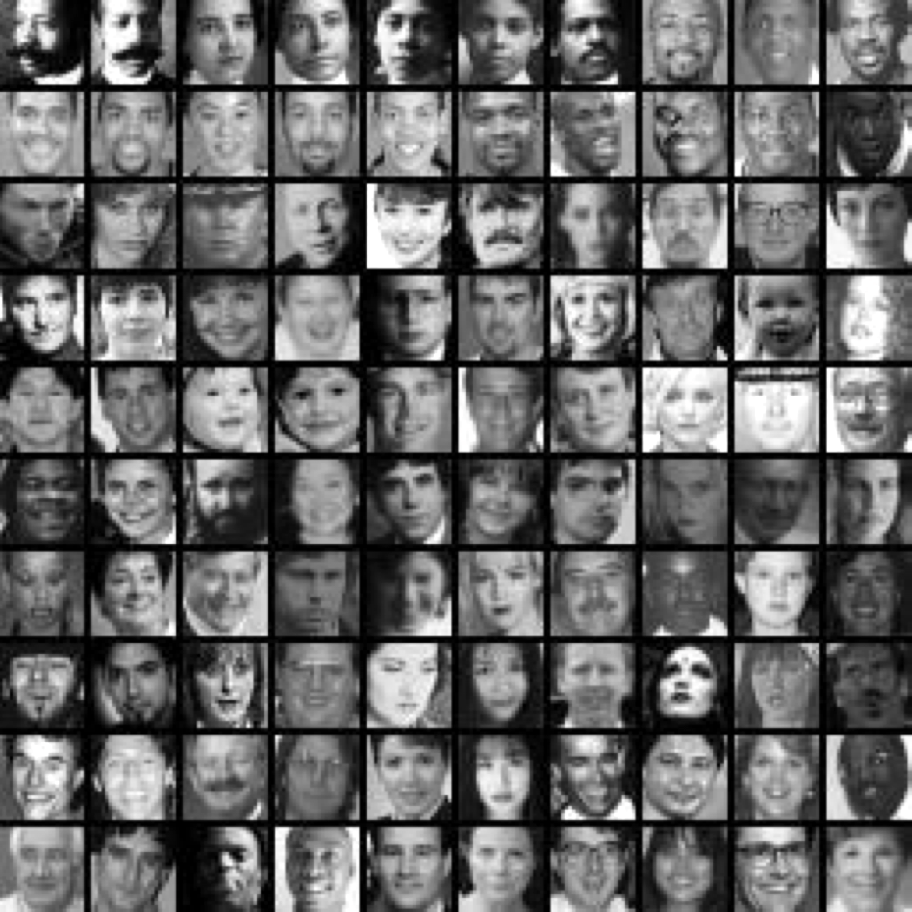
\includegraphics[width=240pt]{chapters/tracking_library_for_the_web/viola_training.png}
  \caption{Example of frontal upright face images used for training \cite{Viola2001}.}
  \label{figure:viola_training}
\end{figure}

A scanning detector was implemented in JavaScript \cite{International2009} and is available on \textit{tracking.js}. The training data used is from OpenCV library \cite{Bradski2000} converted from Extensible Markup Language (XML) \cite{Bray2013} to JavaScript Object Notation (JSON) \cite{Crockford2013}. JSON \cite{Crockford2013} has much superior performance since it's interpreted by JavaScript language \cite{International2009,Crockford2013}. The results of the JavaScript \cite{International2009} implementation can be used in real-time applications, the detector runs at 15 frames per second. For more information about performance see Chapter \ref{cha:evaluation}.

The overall idea of the detection process is that it uses a degenerate decision tree, what Viola and Jones \cite{Viola2001} call ``cascade''. A positive result from the first classifier triggers the evaluation of a second classifier which has also been adjusted to achieve very high detection rates \cite{Viola2001}. A positive result from the second classifier triggers a third classifier, and so on \cite{Viola2001}. The main steps of the scanning algorithm are:

\begin{enumerate}
  \item Create or scale a squared block, initially set to $20\times20$ pixels, by $1.25$ per iteration;
  \item Loop the squared block by $\Delta$ pixels over the image;
  \item For each squared block location, loop the decision tree and evaluate each stage;
  \item A positive result of the stage \cite{Viola2001} triggers the next stage, otherwise stops the stages loop;
  \item If all stages were positively evaluated store that rectangle as a possible face;
  \item Once the decision tree is done, group the overlapping rectangles;
  \item Find the best rectangle of each the group to represent the face. This phase is also known as ``merging phase''.
\end{enumerate}

The final detector is scanned across the image at multiple scales and locations of the image. This process makes sense because the features can be evaluated at any scale with the same cost \cite{Viola2001}. Good results were obtained using a set of scales a factor of $1.25$. Subsequent locations are obtained by shifting the window some number of pixels $\Delta$, for a better accuracy $\Delta=1$ is recommended. We can achieve a significant speedup by setting $\Delta=2$ with only a slight decrease in accuracy, thus this value was set as default value of the JavaScript \cite{International2009} implementation.

Viola and Jones \cite{Viola2001} proposed that for each found possible rectangle representing the face to be partitioned into disjoint subsets data structures. Two detections are in the same subset if their bounding regions overlap \cite{Viola2001}. The corners of the final bounding region are the average of the corners of all detections in the set. In order to perform well on the web, some optimizations were made in the implementation level of the scanning detector. The disjoint set was replaced by an alternative logic that is called ``Minimum Neighbor Area Grouping'' by this thesis. Minimum Neighbor Area Grouping has $O(N^2)$ performance \cite{black2007big} and consists in a loop trough the possible rectangle faces returned by the scanning detector. For each step of the loop compare the current rectangle with all other not yet compared rectangles. If the rectangle area overlaps more than $\eta$ with the compared, by default $\eta=0.5$ (or $50\%$), select the smallest rectangle in area of the comparison. Using the smallest rectangle, guarantees that the best match is much centralized in the face.

For more information about the JavaScript \cite{International2009} implementation, such as evaluation and results, see Chapter \ref{cha:evaluation}.

% subsection contextualization (end)

% section rapid_object_detection (end)

\section{Color Tracking Algorithm} % (fold)
\label{sec:tracking_library_for_the_web:color_tracking_algorithm}

\subsection{Contextualization} % (fold)
\label{sub:tracking_library_for_the_web:color_tracking_algorithm:contextualization}

Colors are part of our lives, they are everywhere in every single object. Being able to use colored objects to control your browser using the user camera is very appealing. For that reason, \textit{training.js} implemented a basic color tracking algorithm that resulted in an real-time frame rate trough a simple and intuitive API.

% subsection contextualization (end)

% section color_tracking_algorithm (end)

% chapter tracking_library_for_the_web (end)
% \appendix
% \chapter{Tracking Library for the Web (tracking.js)} % (fold)
\label{cha:tracking_library_for_the_web}

\section{Contextualization} % (fold)
\label{sec:tracking_library_for_the_web:Contextualization}

The desktop platform is the target environment most commonly addressed when developing AR systems. However, depending on the requirements of an AR application, the use of different execution platforms may be necessary. If the system has to be published to several users, the web platform shows to be more adequate, where the application is executed through the Internet in a web browser \cite{Pablo2013}.
The use of markerless tracking, which is based on natural features of the scene, has also been gaining more space on web targeted AR applications for advertising. The media used in this kind of application needs to be as appealing as possible in order to catch consumers' attention. Markerless tracking satisfies this requirement, since the idea of having a real scene augmented with virtual objects without any artificial elements such as markers added to the environment is very attractive \cite{Pablo2013}. In addition, the product being advertised can be tracked and augmented with virtual elements \cite{Pablo2013}.
Browsers are evolving very fast when compared to the the previous decade \cite{Hickson2013}. JavaScript language \cite{International2009,MDN2013} wasn't prepared to handle typed data structures \cite{TypedArray2013} able to manipulate raw binary data safely \cite{Canvas2013}, all the computational complexity required by AR algorithms was too much for that growing environment. Browsers weren't able to capture audio and video \cite{MediaCapture2013,WebRTC2013} natively, without plugin installation \cite{Flash2013}, an essential feature for AR applications. This reality has changed, this involves the use of several modern browser specifications \cite{Hickson2013,WC2006} as well as implementation of different computer vision algorithms and techniques into the browser environment taking advantage of all those modern APIs \cite{Hickson2013,WC2006}.

In this context, this thesis aims to present the implementation and evaluation of a solution regarding tracking techniques for web targeted AR. The available algorithms and techniques can be used for different applications, such as, detect faces, identify objects and colors and track moving objects. The solution is called \textit{tracking.js}. Some optimizations are discussed and implemented on this work in order to achieve good results when compared with similar implementations in compiled languages.

\subsection{Related Work} % (fold)
\label{sub:tracking_library_for_the_web:related_work}

There are not many web based RA solutions available and registered in the literature. The ones available are mainly focused on fiducial markers \cite{Cho1998}, such as FLARToolKit \cite{Yan2011} and JSARToolkit \cite{JSARToolkit2011}, they both are ports of ARToolKit \cite{Hirokazu2002}. ARToolKit is a desktop library which is useful to make vision-based AR applications \cite{Hirokazu2002}. The Metaio company developed Unifeye Viewer \cite{Metaio2009}, a proprietary plug-in for Flash \cite{Flash2013} that allows the utilization of markerless AR applications on the web. In order to run Flash \cite{Flash2013} based applications, the installation of its plugin is required. Third-party plugins, such as Flash \cite{Flash2013}, are in decadency on modern and mobile web browsers, instead JavaScript \cite{International2009} based solutions are preferred, since they can run in any modern browser without requiring any user effort of installing external software. Some smart-phones don't even support Flash \cite{Flash2013} plugin into their browsers, \eg\ Safari for mobile \cite{Safari2013} is one example of a mobile browser that has banned Flash \cite{Flash2013}.

\begin{enumerate}
    \item FLARToolKit: is a port of the well-known ARToolKit \cite{Hirokazu2002} marker tracking library to ActionScript \cite{Flash2013}, which is the language utilized in the development of Flash \cite{Flash2013} applications for the web. This was the first initiative towards AR solutions for the web \cite{Pablo2013}. Using FLARToolKit \cite{Yan2011}, is possible to develop AR applications that runs on client's browser. A marker based AR example for the web, developed for a marketing campaign of General Electric's company using FLARToolKit, is shown on Figure \ref{figure:flartoolkit}.

    \begin{figure}[!htb]
      \centering
      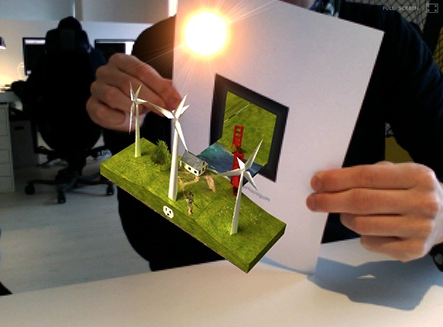
\includegraphics[width=240pt]{chapters/tracking_library_for_the_web/flartoolkit.png}
      \caption{Marker based AR for the web using FLARToolKit.}
      \label{figure:flartoolkit}
    \end{figure}

    \item JSARToolkit: is a JavaScript \cite{International2009} port of FLARToolKit \cite{Yan2011}, operating on canvas images \cite{Canvas2013} and
video element \cite{Hickson2013} contents, provides another marker tracking library. This was the first, open-source, JavaScript \cite{International2009} based, AR solution available for the web. A marker based AR example for the web using JSARToolKit is shown on Figure \ref{figure:jsartoolkit}.

    \begin{figure}[!htb]
      \centering
      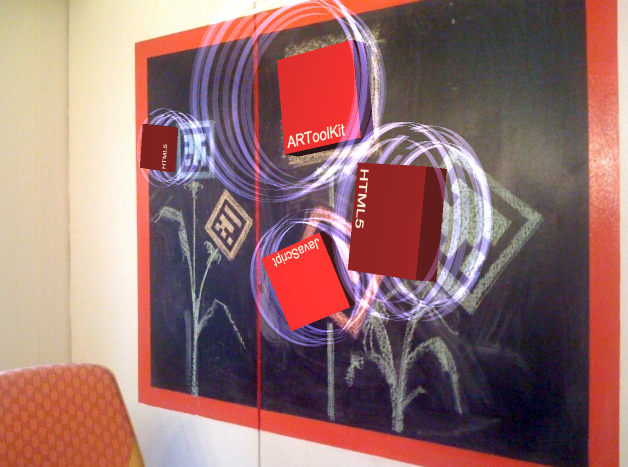
\includegraphics[width=240pt]{chapters/tracking_library_for_the_web/jsartoolkit.png}
      \caption{Marker based AR for the web using JSARToolKit.}
      \label{figure:jsartoolkit}
    \end{figure}

    \item Unifeye Viewer: from Metaio company, offers a robust markerless tracking solution for the web. Unifeye \cite{Metaio2009} also depends on Flash \cite{Flash2013} plugin in order to run on web browsers. A similar example of General Electric's marker based solution, this time markerless based, is shown on Figure \ref{figure:unifeyeviewer}. Note that the 3D image is projected over a magazine cover instead of a fiducial marker \cite{Cho1998}.

    \begin{figure}[!htb]
      \centering
      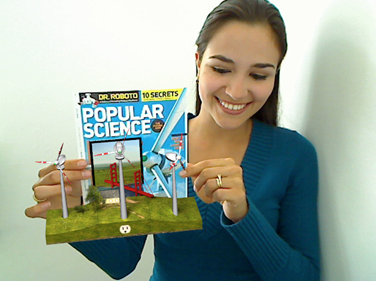
\includegraphics[width=240pt]{chapters/tracking_library_for_the_web/unifeyeviewer.png}
      \caption{Markerless example of image projected over a magazine cover using Unifeye Viewer solution.}
      \label{figure:unifeyeviewer}
    \end{figure}
\end{enumerate}

There is a disadvantage of using marker based AR. Depend on a artificial marker in order to augment the scene with virtual elements is counterintuitive. Commonly, web applications are utilized by novice users that do not have sufficient technical knowledge to perform manual setup, such as print fiducial markers or perform manual initialization for the tracking. FLARToolKit \cite{Yan2011} and JSARToolkit \cite{JSARToolkit2011} are both marker based techniques, using Flash \cite{Flash2013} and JavaScript \cite{International2009}, respectively. FLARToolKit has one more issue which is dependency on Flash \cite{Flash2013} plugin installation. Unifeye Viewer by Metaio, was the only existing solution that provided markerless tracking for the web, although it uses Flash \cite{Flash2013}, excluding it from a potential competitor of \textit{tracking.js}. Markerless tracking techniques do not depend on any artificial marker or advanced user initialization. The space on web targeted AR applications for advertising is gaining more space and the media used in this kind of application needs to be as appealing as possible \cite{Pablo2013}. Making markerless tracking a suitable technique to such applications.

The solution proposed in this thesis, \textit{tracking.js}, provides the first known, open-source, markerless tracking solution for the web that runs entirely in JavaScript \cite{International2009} and HTML5 \cite{Hickson2013}.

% subsection related_work (end)

\subsection{Library Modules} % (fold)
\label{sub:tracking_library_for_the_web:library_modules}

The proposed library is divided in modules in order to allow extension and addition of new features, such as new RA techniques or math utilities. For a better understanding of the library architecture, the current implementation is divided in two packages separating Base from AR classes. Base classes modules are shown in Figure \ref{figure:base_classes} and AR classes in Figure \ref{figure:ar_classes}.

To develop AR applications using only raw JavaScript \cite{International2009} APIs \cite{MDN2013} could be too verbose and complex, \eg\ capturing users' camera and reading its array of pixels. The big amount of steps required for a simple task makes web developers life hard when the goal is to achieve complex implementations. Some level of encapsulation is needed in order to simplify development. The proposed library provides encapsulation for common tasks on the web platform.

The two main available packages splits Base from AR classes. Furthermore, each class of those packages are described. Let's start with the base classes:

\begin{enumerate}
  \item Math: provides common math utilities optimized for the web, such as geometry, linear algebra \cite{Hartley2004} and hamming operations. Typed arrays \cite{TypedArray2013} are used in order to optimize performance, see subsection \ref{sub:basic_concepts:web:javascript_typed_arrays} for more information about typed arrays.
  \item Attribute: allows developers to add attributes to any class through an Attribute interface. The interface adds get and set methods to your class to retrieve and store attribute values, as well as support for change events that can be used to listen for changes in attribute values.
  \item DOMElement: provides a way to create, and manipulate HTML \cite{Hickson2013} DOM nodes \cite{WC2006}. Each DOMElement instance represents an underlying DOM node \cite{WC2006}. In addition to wrapping the basic DOM API \cite{WC2006} and handling cross browser issues, Nodes provide convenient methods for managing styles and subscribing to events.
  \item Canvas: provides an utility class to create, and manipulate HTML5 \cite{Hickson2013} canvas element \cite{Canvas2013}. Each Canvas instance represents an underlying canvas DOM node \cite{Canvas2013}. In addition to wrapping the basic DOM API \cite{WC2006}, also provides methods to extract via \textit{getImageData} method, to loop via \textit{forEach} method, and to set the canvas array of pixels via \textit{setImageData} method.
  \item Video: provides an utility class to create, and manipulate HTML5 \cite{Hickson2013} video element. Each Video instance represents an underlying video DOM node \cite{Canvas2013}. In addition to wrapping the basic DOM API \cite{WC2006}, also provides methods to \textit{play}, \textit{pause} and register tracker algorithms via \textit{track} method. See subsection \ref{sub:basic_concepts:web:audio_and_video} for more information about video element.
  \item VideoCamera: extends all functionalities from Video class with the addition of capturing the user camera via \textit{capture} method. The underlying implementation uses WebRTC \cite{WebRTC2013} and Media Capture and Streams \cite{MediaCapture2013} specifications.
\end{enumerate}

Visual tracking classes includes several computer vision algorithms, such as FAST \cite{RostenFaster2010}, BRIEF \cite{Calonder2010} implementations, homography estimation and others. As the library grows, many other computer vision algorithms are going to be added to the library, such as 3D pose calculation.

\begin{enumerate}
  \item FAST: provides an implementation of Features from Accelerated Segment Test (FAST) \cite{Rosten2010} for features detection via \textit{findCorners(data, threshold)} method, where $data$ is the \textit{ImageData} of the canvas \cite{Canvas2013} frame. It also depends on a $threshold$ argument. The pixel at $p$, see Figure \ref{figure:fast}, is the center of a candidate corner and they are classified if brighter than $p$ by more than the $threshold$.
  \item BRIEF: provides an implementation of Binary Robust Independent Elementary Features (BRIEF) \cite{Calonder2010} for feature extraction via \textit{getDescriptors(data, corners)} method and matching via \textit{match(c1, d1, c2, d2)}, where $data$ is an \textit{ImageData}, and $c1$ and $c2$ are the found corners array return by \textit{FAST.findCorners} method and $d1$ and $d2$ are feature descriptors array return by \textit{BRIEF.getDescriptors} method.
  \item RANSAC: provides an interface used to achieve robust estimation method for homographies and camera pose. There are two available estimation methods implemented that inherits from RANSAC \cite{Hartley2004}, Homography and Pose.
  \item Homography: provides an API to estimate a homography matrix $H$ between images by finding feature correspondences in those images.
  \item Pose: TODO.
  \item ViolaJones: TODO.
  \item Color: TODO.
\end{enumerate}

\begin{figure}[!htb]
    % \tikzumlset{font=\scriptsize}
    \begin{tikzpicture}
        \begin{umlpackage}{Base classes}

            \umlclass[y=-50pt,x=190pt]{Math}{}{
              createIdentityMatrix(size) : Matrix\\
              distance(x1, y1, x2, y2) : Number\\
              getDeterminant(Matrix) : Number\\
              getInverse(Matrix) : Matrix\\
              hammingDistance(n1, n2) : Number\\
              hammingWeight(number) : Number\\
              ...
            }

            \umlclass{Attribute}{}{
              get(name) : Object\\
              set(name, value) : void \\
            }

            \umlclass[y=-100pt]{DOMElement}{
              width : Number\\
              height : Number\\
              visible : boolean\\
            }{
              show() : void\\
              hide() : void \\
            }

            \umlclass[y=-220pt,x=180pt]{Canvas}{
              context : Object
            }{
              forEach(data, callback) : void\\
              getImageData(x, y, width, height) : ImageData \\
              setImageData(data, x, y) : void\\
            }

            \umlclass[y=-335pt]{Video}{}{
              play() : void\\
              pause() : void\\
              track(tracker) : void \\
              getVideoCanvasImageData(x, y, width, height) : ImageData \\
            }

            \umlclass[y=-335pt,x=220pt]{VideoCamera}{}{
              capture() : void \\
            }

        \end{umlpackage}

        \umlinherit[geometry=-|]{DOMElement}{Attribute}
        \umlinherit[geometry=-|]{Canvas}{DOMElement}
        \umlinherit[geometry=-|]{Video}{DOMElement}
        \umlinherit[geometry=|-]{VideoCamera}{Video}
    \end{tikzpicture}
    \caption{Base classes of tracking.js library.}
    \label{figure:base_classes}
\end{figure}

\begin{figure}[!htb]
    % \tikzumlset{font=\scriptsize}
    \begin{tikzpicture}
        \begin{umlpackage}{Visual tracking classes}

            \umlclass{FAST}{}{
              findCorners(data, threshold) : Array\\
            }

            \umlclass[y=-70pt]{BRIEF}{}{
              getDescriptors(data, corners) : Array\\
              match(c1, d1, c2, d2) : Array\\
            }

            \umlclass[y=-150pt]{ViolaJones}{}{
              find() : Array\\
              evalStage() : boolean\\
            }

            \umlclass[y=-225pt]{Color}{}{
              find() : Array\\
            }

            \umlclass[x=200pt]{RANSAC}{}{
              find(matches) : void\\
              score() : Number\\
            }

            \umlclass[y=-90pt,x=200pt]{Homography}{}{
                score(H, matches) : Number\\
            }

            \umlclass[y=-170pt,x=200pt]{Pose}{}{
              find(points2d, points3d) : void\\
            }

        \end{umlpackage}

        \umlinherit[geometry=-|]{Homography}{RANSAC}
        \umlinherit[geometry=-|]{Pose}{RANSAC}
    \end{tikzpicture}
    \caption{Visual tracking classes of tracking.js library.}
    \label{figure:ar_classes}
\end{figure}

\newpage

% subsection library_modules (end)

% section contextualization (end)

\section{Markerless Tracking Algorithm} % (fold)
\label{sec:tracking_library_for_the_web:marker_less_tracking_algorithm}

\subsection{Contextualization} % (fold)
\label{sub:tracking_library_for_the_web:marker_less_tracking_algorithm:contextualization}

Lorem ipsum dolor sit amet, consectetur adipisicing elit.

% subsection contextualization (end)

\subsection{Feature Detector} % (fold)
\label{sub:tracking_library_for_the_web:marker_less_tracking_algorithm:feature_detector}

This technique relies on matching individual features across images and are therefore easy to increase robustness against partial occlusions or matching errors. Illumination invariance is also simple to achieve. Feature points detection is used as the first step of many vision tasks such as tracking, localization, image matching and recognition. In this article we call ``feature'' or ``keypoint'' to refer to a point of interest in two dimensions.

For each frame, the object features are matched by localizing feature templates in search windows around hypothesized locations \cite{Lepetit2005}. The method to extract feature points suggested in Features from Accelerated Segment Test (FAST) \cite{Rosten2010}. FAST \cite{RostenFaster2010} hypothesizes the matches using corner detection. A large number of corner detectors exist in the literature. However, we have a strong interest in real time frame rate applications which computational resources are required requisites. The approach proposed by FAST \cite{RostenFaster2010} allows the detector to produce a suite of high-speed detectors which we currently use for real-time tracking and AR label placement \cite{Calonder2010}. In particular, it is still true that when processing live video streams at full frame rate, existing feature detectors leave little if any time for further processing, even despite the consequences of Moore's Law \cite{Rosten2010}.

To show that speed can been obtained without necessarily sacrificing the quality of the feature detector, in Chapter \ref{cha:evaluation}, we compare our detector, to a variety of well-known detectors. A number of the detectors described below compute a corner response, (1) Edge based corner detectors, corresponds to the boundary between two regions; (2) Gray level derivative based detectors, the assumption that corners exist along edges is an inadequate model for patches of texture and point like features, and is difficult to use at junctions. Therefore a large number of detectors operate directly on gray level images without requiring edge detection; and (3) Direct gray level detectors, Another major class of corner detectors work by examining a small patch of an image to see if it ``looks'' like a corner \cite{Rosten2010}.

The thesis choice was (3) Direct gray level detectors. It works by testing a small patch of an image to see if it could be a corner. The detector is evaluated using a circle surrounding the candidate pixel, the test is based on whether the concentric contiguous arcs around the pixel are significantly different from the central pixel $p$ \cite{Rosten2010}. To classify $p$ as a corner should exists a set of $n$ contiguous pixels in the circle which are all brighter than the intensity of the candidate pixel $I_{p} + t$ (threshold), or all darker than $I_{p} - t$ \cite{Rosten2010}.

The number of contiguous tested pixels could vary accordingly \cite{Rosten2010}, being more common to be FAST-$12$ or FAST-$9$. Empirically, FAST-$9$ showed to have a good repeatability and a better efficiency on the web. The repeatability of found feature points is also important because determines whether the technique is useful in a real-world application.

This detector in itself exhibits high performance, but there are several weaknesses: (1) This high-speed test does not reject as many candidates; (2) The efficiency of the detector will depend on the ordering of the questions and the distribution of corner appearances; and (3) Multiple features are detected adjacent to one another \cite{Rosten2010}.

On Figure \ref{figure:fast}, the highlighted squares are the pixels used in the corner detection. The pixel at $p$ is the central pixel. The arc is indicating that the dashed line passes through FAST-$n$, let $n$ be $9$ or $12$ contiguous pixels which are brighter or darker than $p$ \cite{Rosten2010}.

\begin{figure}[!htb]
  \centering
  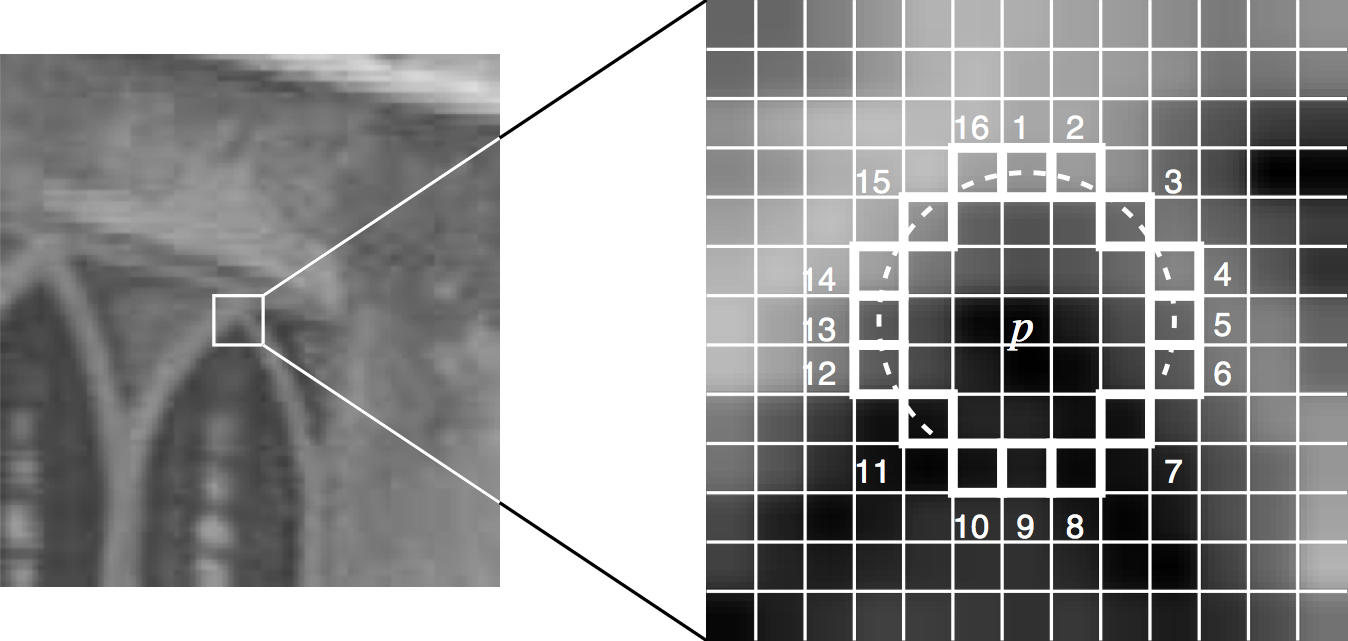
\includegraphics[width=380pt]{chapters/tracking_library_for_the_web/fast.png}
  \caption{Point segment test corner detection in an image patch \cite{Glass2013}.}
  \label{figure:fast}
\end{figure}

% subsection feature_detector (end)

\subsection{Feature Extractors} % (fold)
\label{sub:tracking_library_for_the_web:marker_less_tracking_algorithm:feature_extractors}

To estimate motion, one can then match sets of features \{$m_{i}$\} and \{$m'_{j}$\} extracted from two images taken from similar, and often successive, viewpoints. A classical procedure \cite{Calonder2010} runs as follows. For each point \{$m_{i}$\} in the first image, search in a region of the second image around location \{$m_{i}$\} for point \{$m'_{j}$\}. The search is based on the similarity of the local image windows, also knowns as kernel windows, centered on the points, which strongly characterizes the points when the images are sufficiently close \cite{Lepetit2005}.

\begin{figure}[!htb]
  \centering
  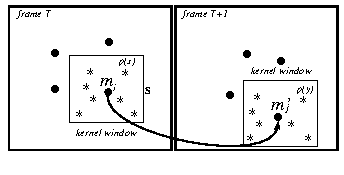
\includegraphics[width=\linewidth]{chapters/tracking_library_for_the_web/BRIEF.pdf}
  \caption{BRIEF \cite{Lepetit2005} feature extractor.}
  \label{figure:BRIEF}
\end{figure}

The feature matching used in the case studies performed in this work search for correspondent points in the current frame. Only points that are highly descriptive invariant features, called keypoints, are tested. Those keypoints were detected using FAST \cite{Rosten2010} in Section \ref{sub:tracking_library_for_the_web:marker_less_tracking_algorithm:feature_detector}. After the keypoints are detected they need to be described and the respective matching point should be found. Since web and handled devices have limited computational power having local descriptors that are fast to compute, to match and being memory efficient are important aspects, for that reason, was used an efficient method called Binary Robust Independent Elementary Features (BRIEF) \cite{Calonder2010}.

To generate the binary string for each key-point found in the smoothed frame, the individual bits are obtained by comparing the intensities of pairs of points, $(\textbf{p}; x, y)$, represented by $\ast$ symbol on Figure \ref{figure:BRIEF}, along the kernel window centered on each key-point without requiring a training phase.
Empirically, this technique shows that $256$ or even $128$ bits \cite{Calonder2010}, often suffice to obtain very good matching results. The best spatial arrangement of the tested (\textbf{x}, \textbf{y})-pairs of points are reach when selected based on an isotropic Gaussian distribution \cite{Calonder2010}. To compute the Gaussian distribution can be time consuming. As an optimization proposed by this article, the Gaussian distribution could be simply replaced by a random function due to its random characteristics.

To generate the binary strings is defined test $\tau$ on patch \textbf{p} of size \textbf{S $\times$ S} as

$$\tau(\textbf{p}; x, y) :=
\begin{cases}
  1 &\mbox{if}\quad \textbf{p(x)} < \textbf{p(y)},\\
  0 &\mbox{otherwise}
\end{cases}$$

where \textbf{p(x)} is the pixel intensity. The set of binary tests is defined by the $n_{d}$ (\textbf{x}, \textbf{y})-location pairs uniquely chosen during the initialization. The $n_{d}$-dimensional bit-string is our BRIEF descriptor for each key-point

$$f_{n_{d}}(\textbf{p}) := \sum_{1 \le i \le n_{d}} 2^{i-1} \tau(\textbf{p}; x, y).$$

In \cite{Calonder2010}, $n_{d}= 128, 256, 512$ were used in the tests and any of those values yield good compromises between speed, storage efficiency, and recognition rate. In this article, $n_{d}= 128$ was used, since it presented good matching results and performance. The number of bytes required to store the descriptor can be calculated by $k = n_{d}/8$, proving that BRIEF is also a memory-efficient method. Detailed results can be found in Chapter \ref{cha:evaluation}.

Once each keypoint is described with its binary string \cite{Calonder2010}, they need to be compared with the closest matching point. Distance metric is critical to the performance of intrusion detection systems. Thus using binary strings reduces the size of the descriptor and provides an interesting data structure that is fast to operate with whose similarity can be measured by the Hamming distance which, on desktop implementations, the computation time could be driven almost to zero using the POPCNT instruction from SSE4.2 \cite{Intel2007}. Only the latest Intel Core i7 CPUs support this instruction.

The Hamming distance is an important step on feature matching, it provides a fast and memory-efficient way to calculate distance between binary strings. Given two image patches $x$ and $y$, denote their binary descriptors as $b(x) \in \{0,1\}^n$ and $b(y) \in \{0,1\}^n$ respectively. Then their Hamming distance is computed by:

$$Ham(x, y)=\sum_{i=1}^{n}b_i(x)\otimes b_i(y)$$

In which $n$ is the dimension of binary descriptor and stands for bitwise XOR operation. According to the definition of Hamming distance, all the elements of a binary descriptor contribute equally to the distance. From the hamming distance, the Hamming weight can be calculated. It is used to find the best feature point match. Here, is generalized the Hamming distance to the weighted Hamming:

$$WHam(x, y)=\sum_{i=1}^{n}w_i(b_i(x)\otimes b_i(y))$$

Where $w_i$ is the weight of the $i$th element. The goal is to learn $w_i,i=1,2\cdots,n$ for the binary descriptor (BRIEF) based on a set of feature points. By assigning different weights to binary codes, what we expect is to obtain a distance space in which the distances of matching patches are less than those of non-matching patches.

% subsection feature_extractors (end)

\subsection{Homography Estimation} % (fold)
\label{sub:tracking_library_for_the_web:marker_less_tracking_algorithm:homography_estimation}

Typically, homographies are estimated between images by finding feature correspondences in those images. A 2D point $(x,y)$ in an image can be represented as a 3D vector $\textbf{x} = (x_1, x_2, x_3)$ where $x = \frac{x_1}{x_3}$ and $y = \frac{x_2}{x_3}$ \cite{Homography2009}. This is called the homogeneous representation of a point and it lies on the projective plane $P^2$. A homography is an invertible mapping of points and lines on the projective plane $P^2$. Hartley and Zisserman \cite{Hartley2004} provide the specific definition that a homography is a mapping from $P^2$ → $P^2$ is a projectivity if and only if there exists a non-singular $3\times3$ matrix $H$ such that for any point in $P^2$ represented by vector $\textbf{x}$ it is true that its mapped point equals $H\textbf{x}$. It should be noted that $H$ can be changed by multiplying by an arbitrary non-zero constant without altering the projective transformation. Thus $H$ is considered a homogeneous matrix and only has $8$ degrees of freedom even though it contains $9$ elements.

The method chosen to solve the homography estimation was the Direct Linear Transformation (DLT) \cite{Impa2009,Hartley2004} algorithm. The DLT algorithm is a simple algorithm used to solve for the homography matrix $H$ given a sufficient set of point correspondences \cite{Homography2009}.

Since we are working in homogeneous coordinates, the relationship between two corresponding points $\textbf{x}$ and $\textbf{x'}$ can be re-written as \cite{Homography2009}:

$$c\begin{pmatrix}u\\ v\\ 1\\\end{pmatrix} = H\begin{pmatrix}x\\ y\\ 1\\\end{pmatrix} \;\; \forall \;\; H=\begin{pmatrix}h1 & h2 & h3\\ h4 & h5 & h6\\ h7 & h8 & h9\\\end{pmatrix},$$

where $c$ is any non-zero constant, $(\; u \; v \; 1 \;)^T$ represents $\textbf{x'}$, $(\; x \; y \; 1 \;)^T$ represents $\textbf{x}$. Dividing the first row of equation (2.1) by the third row and the second row by the third row we get the following two equations \cite{Homography2009}:

\begin{equation}
\label{eq:homography1}
-h1x-h2y-h3 +(h7x+h8y+h9)u=0
\end{equation}
\begin{equation}
\label{eq:homography2}
-h4x-h5y-h6 +(h7x+h8y+h9)u=0
\end{equation}

Equations (\ref{eq:homography1}) and (\ref{eq:homography2}) can be written in matrix form as $A_i\textbf{h}=0$. Where,

$$A_i=\begin{pmatrix}-x & -y & -1 & 0 & 0 & 0 & ux & uy & u\\0 & 0 & 0 & -x & -y & -1 & vx & vy & v\end{pmatrix}$$

and

$$\textbf{h}=\begin{pmatrix}h1 & h2 & h3 & h4 & h5 & h6 & h7 & h8 & h9\end{pmatrix}.$$

Since each point correspondence provides $2$ equations, $4$ correspondences are sufficient to solve for the $8$ degrees of freedom of $H$. JavaScript typed arrays, defined in Section \ref{sub:basic_concepts:web:javascript_typed_arrays}, were used in the homography estimation implementation for better performance results.

% subsection homography_estimation (end)

\subsection{Random Sample Consensus (RANSAC)} % (fold)
\label{sub:tracking_library_for_the_web:marker_less_tracking_algorithm:ransac}

RANSAC (Random Sample Consensus) \cite{Hartley2004} is the most commonly used robust estimation method for homographies according to \cite{Homography2009}. The idea of the algorithm is pretty simple; For a number of iterations, a random sample of $4$ correspondences is selected and a homography $H$ is computed from those four correspondences. Each other correspondence is then classified as an inlier or outlier depending on its concurrence with $H$. After all of the iterations are done, the iteration that contained the largest number of inliers is selected. $H$ can then be recomputed from all of the correspondences that were consider as inliers in that iteration \cite{Homography2009}.

One important step when applying the RANSAC algorithm described above is to decide how to classify correspondences as inliers or outliers. In the implementation for the web only assign the geometric distance \cite{Homography2009} threshold, $t$, between $\textbf{x'}$ and $H\textbf{x}$ was enough. Hartley and Zisserman \cite{Hartley2004} provides more details about RANSAC.

Another issue is to decide how many iterations to run the algorithm, it's not required to try every combination of 4 correspondences. The goal becomes to determine the number of iterations, $N$, that ensures with a probability $p$ that at least one of the random samples will be free from outliers. $N=100$ was used on the web implementation.

% subsection ransac (end)

% section marker_less_tracking_algorithm (end)

\section{Rapid Object Detection (Viola Jones)} % (fold)
\label{sec:tracking_library_for_the_web:rapid_object_detection}

\subsection{Contextualization} % (fold)
\label{sub:tracking_library_for_the_web:rapid_object_detection:contextualization}

Rapid Object Detection \cite{Viola2001} technique, much known as Viola Jones \cite{Viola2001}, brings together new algorithms and insights to construct a library for robust and extremely rapid object detection. What has motivated this technique to be added to \textit{tracking.js} library was the task of face detection. Surprisingly, the algorithm became robust enough to detect any training data \cite{Viola2001}, not only for faces. Currently, \textit{tracking.js} supports, face, eyes, upper body and palm detection.

In order to scan faces, eyes or palm from images, a training phase is required. The training phase generate cascading stages. The cascade are constructed by training classifiers using AdaBoost \cite{Viola2001} and then adjusting the threshold to minimize false negatives. OpenCV library \cite{Bradski2000} has some open-source training data, therefore doubling efforts on training is unnecessary, \ie\ the face training set consisted of 4916 faces, extracted from images downloaded during a random crawl of the world wide web \cite{Viola2001}. Those faces were scaled and aligned to a base resolution of $24$ by $24$ pixels \cite{Viola2001}, see Figure \ref{figure:viola_training}. Training is not the focus of this work, the algorithm to scan the faces is. The training data itself is useless if a Scanning Detector \cite{Viola2001} is not available, the scanning is what makes the rapid object detection.

\begin{figure}[!htb]
  \centering
  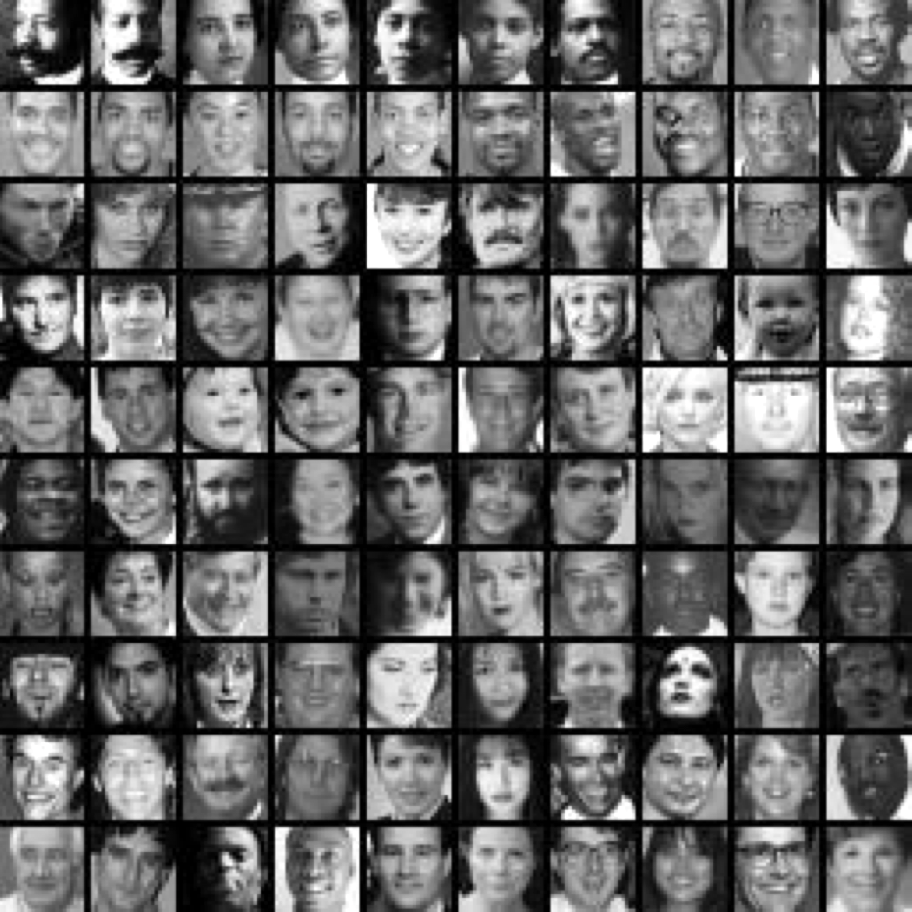
\includegraphics[width=240pt]{chapters/tracking_library_for_the_web/viola_training.png}
  \caption{Example of frontal upright face images used for training \cite{Viola2001}.}
  \label{figure:viola_training}
\end{figure}

A scanning detector was implemented in JavaScript \cite{International2009} and is available on \textit{tracking.js}. The training data used is from OpenCV library \cite{Bradski2000} converted from Extensible Markup Language (XML) \cite{Bray2013} to JavaScript Object Notation (JSON) \cite{Crockford2013}. JSON \cite{Crockford2013} has much superior performance since it's interpreted by JavaScript language \cite{International2009,Crockford2013}. The results of the JavaScript \cite{International2009} implementation can be used in real-time applications, the detector runs at 15 frames per second. For more information about performance see Chapter \ref{cha:evaluation}.

The overall idea of the detection process is that it uses a degenerate decision tree, what Viola and Jones \cite{Viola2001} call ``cascade''. A positive result from the first classifier triggers the evaluation of a second classifier which has also been adjusted to achieve very high detection rates \cite{Viola2001}. A positive result from the second classifier triggers a third classifier, and so on \cite{Viola2001}. The main steps of the scanning algorithm are:

\begin{enumerate}
  \item Create or scale a squared block, initially set to $20\times20$ pixels, by $1.25$ per iteration;
  \item Loop the squared block by $\Delta$ pixels over the image;
  \item For each squared block location, loop the decision tree and evaluate each stage;
  \item A positive result of the stage \cite{Viola2001} triggers the next stage, otherwise stops the stages loop;
  \item If all stages were positively evaluated store that rectangle as a possible face;
  \item Once the decision tree is done, group the overlapping rectangles;
  \item Find the best rectangle of each the group to represent the face. This phase is also known as ``merging phase''.
\end{enumerate}

The final detector is scanned across the image at multiple scales and locations of the image. This process makes sense because the features can be evaluated at any scale with the same cost \cite{Viola2001}. Good results were obtained using a set of scales a factor of $1.25$. Subsequent locations are obtained by shifting the window some number of pixels $\Delta$, for a better accuracy $\Delta=1$ is recommended. We can achieve a significant speedup by setting $\Delta=2$ with only a slight decrease in accuracy, thus this value was set as default value of the JavaScript \cite{International2009} implementation.

Viola and Jones \cite{Viola2001} proposed that for each found possible rectangle representing the face to be partitioned into disjoint subsets data structures. Two detections are in the same subset if their bounding regions overlap \cite{Viola2001}. The corners of the final bounding region are the average of the corners of all detections in the set. In order to perform well on the web, some optimizations were made in the implementation level of the scanning detector. The disjoint set was replaced by an alternative logic that is called ``Minimum Neighbor Area Grouping'' by this thesis. Minimum Neighbor Area Grouping has $O(N^2)$ performance \cite{black2007big} and consists in a loop trough the possible rectangle faces returned by the scanning detector. For each step of the loop compare the current rectangle with all other not yet compared rectangles. If the rectangle area overlaps more than $\eta$ with the compared, by default $\eta=0.5$ (or $50\%$), select the smallest rectangle in area of the comparison. Using the smallest rectangle, guarantees that the best match is much centralized in the face.

For more information about the JavaScript \cite{International2009} implementation, such as evaluation and results, see Chapter \ref{cha:evaluation}.

% subsection contextualization (end)

% section rapid_object_detection (end)

\section{Color Tracking Algorithm} % (fold)
\label{sec:tracking_library_for_the_web:color_tracking_algorithm}

\subsection{Contextualization} % (fold)
\label{sub:tracking_library_for_the_web:color_tracking_algorithm:contextualization}

Colors are part of our lives, they are everywhere in every single object. Being able to use colored objects to control your browser using the user camera is very appealing. For that reason, \textit{training.js} implemented a basic color tracking algorithm that resulted in an real-time frame rate trough a simple and intuitive API.

% subsection contextualization (end)

% section color_tracking_algorithm (end)

% chapter tracking_library_for_the_web (end)
\begin{singlespace}
\bibliography{references}
\bibliographystyle{plain}
\end{singlespace}
\end{document}